\documentclass[a4paper,12pt]{report}
\setcounter{secnumdepth}{3} % Ensure subsubsections are numbered
\setcounter{tocdepth}{3} %per a que surtin subseccions en index (3.4.2.1 apareix amb depth 3)
\usepackage[utf8]{inputenc}
\usepackage[spanish]{babel}  % Cambia el idioma a español
\usepackage{geometry}
\usepackage{setspace}
\usepackage{titlesec}
\usepackage{graphicx}
\usepackage{hyperref} % Paquete para enlaces clicables
\usepackage{placeins} % per a les float barrier, que no es moguin les imatges.
\usepackage{titlesec}  % Paquete para personalizar títulos
\usepackage{float}  %pquete para que las figuras no se de splacen
\usepackage{listings} %para poner entronos de codigo 
\usepackage{multirow} %per poder combinar cel·les d'una taula

\titleformat{\chapter}[hang] % Configuración para reducir el espacio superior de los capítulos
{\normalfont\huge\bfseries} % Formato de la fuente y tamaño del capítulo
{Capítulo \thechapter}{0pt}{\huge}  % Sin espacio entre "Capítulo X" y el título
\titlespacing*{\chapter}{0pt}{-20pt}{20pt} % Ajustes de espacio antes, después, y debajo del título




\usepackage{xcolor} % Para definir colores personalizados

% Configuración del estilo para Git
\lstset{
	language=bash,                   % Usa Bash para sintaxis similar a Git
	basicstyle=\ttfamily\small,      % Texto monoespaciado y pequeño
	keywordstyle=\bfseries,          % Palabras clave en negrita
	commentstyle=\color{gray},       % Comentarios en gris
	morekeywords={git, clone, add, branch, checkout, commit, push}, % Palabras clave de Git
	showstringspaces=false           % No mostrar espacios en cadenas de texto
}



% Configuración de márgenes
\geometry{left=3cm, right=3cm, top=2.5cm, bottom=2.5cm}

% Configuración de espacios
\setstretch{1.15}


% Configuración de formato de títulos
\titleformat{\chapter}[display]
{\normalfont\bfseries\Huge}
{}{0pt}{\Huge}

\hypersetup{
	colorlinks=true,        % Colorear enlaces
	linkcolor=blue,         % Color de los enlaces internos
	urlcolor=blue,          % Color de los enlaces externos (URLs)
	pdftitle={Memoria Proyecto}, % Título del PDF
	pdfauthor={Jorge Muñoz Carrión, Santiago Sánchez Sans} % Autor
}

\begin{document}
	
	

	
	
	
	% Portada
	\begin{titlepage}
		\begin{center}

			
			\vspace*{5cm} 

			\LARGE{Creación de un dashboard para usuarios del ticket digital de Mercadona con visualización de la evolución temporal de precios en productos habitualmente adquiridos, costes de compras por intervalos temporales y gastos por áreas de producto.}
			
			\vfill
			
		\begin{flushright}
			\large{\textbf{Santiago Sánchez Sans}}
			
			\large{\textit{Ciclo formativo en desarrollo de aplicaciones web}}
			
			\large{Memoria del Proyecto de DAW}
			
			\large{IES Abastos. Curso 2024/25. Grupo 7S. 25 de Mayo de 2025}
			
			\large{Tutor Individual: Carlos Furones}
		\end{flushright}

			
			
			% Fecha
			
			
		\end{center}
	\end{titlepage}
	
	
	
	
	
	
	
	
	
	% Página de agradecimientos / aclaración
	\clearpage
	\thispagestyle{empty}  % Sin número de página
	\begin{center}
		\vspace*{3cm}
		
		{\LARGE \textbf{Agradecimientos}} % Puedes cambiar el título
		
		\vspace{1cm}
		
		\begin{minipage}{0.8\textwidth}
			\large
			Quiero agradecer a mi padre y a mi madre por su apoyo incondicional en la realización de este grado superior a tiempo completo, que esperemos permita consumar un cambio profesional del ámbito de la Psicología a la informática.
		\end{minipage}
		
		\vspace{4cm}
		
		{\LARGE \textbf{Mensaje para el lector}} % Puedes cambiar el título
		
		\vspace{1cm}
		
		\begin{minipage}{0.8\textwidth}
			\large
			La redacción íntegra de esta memoria se ha hecho a mano. No se ha utilizado inteligencia artificial para la redacción de ninguna frase, ni revisión gramatical ni ortográfica. Se insta al lector a considerarla el resultado del esfuerzo y trabajo constante a lo largo de los meses de marzo a mayo de 2025 (en paralelo con las prácticas a tiempo completo en Lãberit) y valorarla con su idiosincracia -incluyendo sus imperfecciones-.
		\end{minipage}
		
		\vspace*{4cm}
		
		

	\end{center}
	\clearpage
	
	
	
	
	
	
	
	
	
	
	
	
	
	
	
	
	
	
	
	
	
	
	
	
	
	

	
	% Índice
	\tableofcontents
	\newpage
	
	
	
	
	
	
	
	
	% Per a conseguir que els espais apliquin solsament a les seccions no a l'index
	\begingroup
	\setlength{\parskip}{.7em}
	
	
	% Capítulos y secciones
	\pagenumbering{arabic}
	
	
	\chapter{Identificación de objetivos}

		\section{¿Qué es el ticket digital de Mercadona?}
		
		Mercadona implementa un sistema de tickets digitales que vinculan la tarjeta de débito a un correo electrónico. Cualquier usuario del supermercado que quiera utilizar el ticket digital solamente deberá facilitar estos dos datos y el supermercado le enviará por correo electrónico los tickets de las posteriores compras hechas en cualquier establecimiento de Mercadona.
		
		Las ventajas para el usuario y para el supermercado de tener un ticket digital son evidentes: el cliente no perderá los tickets de cara a devoluciones, no deberá esperar a su impresión después del pago y no se verá expuesto a la tinta del texto del ticket físico: que al menos por allá en 2019 la comisión europea ya alertaba de su peligrosidad \cite{EU_Parliament_2019} a partir de un estudio de la Universidad de Granada que hallaba alto contenido de Bisfenol-A\footnote{Es un químico que es un disruptor del sistema endocrino.} en los tickets de compra de distintos paises \cite{Molina-Molina2019}\cite{CanalUGR}.
		
		Las ventajas de la adopción masiva del ticket digital para el supermercado y el trabajador también son claras: se evita el derroche de papel, se impide que los cajeros estén expuestos a químicos que constituyan un riesgo laboral y, finalmente, se consigue acortar los tiempos de cola mejorando la experiencia de los clientes y asegurando su regreso futuro.
		
		
		
		\section{Identificación de necesidades}
		\label{section:identificacionNecesidades}
		
		Los tickets de cada usuario del ticket digital de Mercadona se acumulan de forma recurrente en su correo electrónico. A pesar de contener información valiosa de cara a la planificación de gastos, este formato digital solamente responde a ventajas operativas para el supermercado y cliente del mismo; pero no ha mejorado todavía la asimilación ni la interpretación de los datos por parte del cliente: este no puede visualizar lo que ha gastado a lo largo de un período temporal, ni la evolución de los precios de los productos que adquiere, ni los supermercados en los que ha comprado, ni las veces que lo ha hecho, etc.
		
		Con un formato estructurado como el que ya tienen a día de hoy los tickets digitales podemos sacar muchísima información y presentársela al cliente de forma clara y visual: los asuntos de los correos que contienen los tickets tienen un formato estándar y predecible, y dentro de cada correo electrónico se encuentra un solo PDF con el desglose de la compra (producto, unidades vendidas, establecimiento, etc.) que espera ser minado y analizado.
 
		\section{Objetivos del proyecto} % OBLIGAT
		\label{section:objetivosProyecto}
		
		Este proyecto quiere responder a estas necesidades. Para ello se plantea la Creación de un \textit{dashboard} o ``cuadro de mando'' en forma de aplicación web para que un usuario del ticket digital de Mercadona pueda visualizar la evolución de precios de los productos adquiridos, el coste promedio de sus compras por períodos temporales y sus distribuciones de gastos a partir de los tickets digitales guardados en una base de datos.
		
		A grandes rasgos, los \textbf{Objetivos principales} del proyecto son proporcionar al usuario del ticket digital una herramienta que muestre en gráficos visuales:

					
		\begin{itemize}
			\setlength{\itemsep}{-.5em}
			\item \textbf{La evolución de precios} (inflación) a lo largo del tiempo en los productos habitualmente comprados en el mismo establecimiento\footnote{La evolución de precios se mostrará solamente para un mismo centro de Mercadona, dado que distintos centros pueden cambiar los nombres de los productos (por ejemplo, en Cataluña…).}.
			\item \textbf{Evolución del gasto} total del usuario a lo largo del tiempo por períodos temporales.
		\end{itemize}
		
		Más concretamente los subobjetivos los mostramos en forma de requisitos en el apartado \ref{sec:requisitosAplicacion}
		
		

		
		

		
		
		
		
		
		
		
		
		
		
			%IDENTIFICAR OBJECTIUS  %OBLIGAT
			%JUSTIFICAR OBJECTIUS   %OBLIGAT
			
			
	
		
	

		



		
	

		
	

		


		

		
		
		
		
	
	\chapter{Diseño del proyecto}  %OBLIGAT
	
		
				

		
		Como veremos en el apartado \ref{sec:analisisRealitatLocal}, el motivo por el que se ha usado principalmente Java como lenguaje de back-end y Spring Boot como framework está vinculado con el análisis de la realidad local: tanto en la probabilidad de inserción laboral futura como en economía de tiempo durante la realización de las prácticas.
		
		Asimismo, de los objetivos principales de los que hemos hablado en la sección \ref{section:objetivosProyecto} hemos derivado una serie de requisitos funcionales de la aplicación, que se verán en el apartado \ref{sec:requisitosAplicacion}
		
		\section{Análisis de la realidad local}
		\label{sec:analisisRealitatLocal}
		
		Esta aplicación tiene muchísimo contenido de back-end. Por ello, la elección del lenguaje de programación para este era importante y obedece a criterios puramente estratégicos. 
		
		En primer lugar, se ha utilizado el lenguaje de programación Java y el framework Spring Boot porque en el equipo de desarrollo de software en el que me he integrado para las prácticas en Lãberit me estoy formando justamente en este lenguaje y framework. 
		
		En segundo lugar, el tiempo de formación inicial en estas prácticas ha entrañado un curso de Spring Boot excesivamente introductorio, y se estimó que la única forma de ganar conocimientos reales era desarrollar una aplicación de back-end completa y segura con el framework, desde cero. De este modo, el salto futuro a una posición más integrada en el equipo de prácticas debería ser más probable; y aprovechando el solapamiento existente en el desarrollo del sistema de gestión de usuarios de mercApp y los contenidos del curso de Spring Boot mandado desde Lãberit han permitido realizar parte de este back-end durante el primer mes de prácticas en la empresa.
			
		En tercer lugar, la elección de Java como lenguaje de back-end en lugar de PHP viene motivada porque otras empresas de la zona utilizan el framework Spring Boot como framework (Mercadona tech, una de ellas). No es de extrañar que esto pase, dado que es el lenguaje que Imma Cabanes nos enseñó en primer curso en Abastos y también el lenguaje que se enseña en primer curso a los estudiantes del grado de ingeniería informática de la Universitat Politécnica de Valencia. Ello implica que el ecosistema tecnológico valenciano se nutre de forma orgánica de desarrolladores Java salidos de la academia.
		
		En cuarto lugar, apostar por Java como lenguaje de back-end es un caballo ganador en forma de crecimiento profesional al ser un lenguaje sólido y de largo recorrido no solo en Valencia sino en muchos países de Europa\footnote{Este fue uno de los motivos que me hizo contactar con Lãberit para hacer las prácticas: poder tocar back-end con Java y Spring Boot.}. No es un lenguaje que vaya por modas y ejercitarlo puede permitir iniciar una carrera enfocada en una tecnología que no se prevé que desfallezca en un futuro cercano.
		
		
		
		
		\section{Requisitos Funcionales}
		
			\textit{NOTA: Los requisitos presentes en el siguiente subapartado se suman a los requisitos que de forma tácita se sobreentiende que debe tener una aplicación de un proyecto final de grado superior; es decir: tener un front-end, un back-end con sistema de registro de usuarios, un login con buenas prácticas en materia de seguridad y una base de datos.}
		
		
			\subsection{Requisitos de la aplicación}
			\label{sec:requisitosAplicacion}
			
		

			

			
		
			
			\textbf{REQUISITO A:} Mostrar\textbf{ \textit{evolución de los precios}} de los productos unitarios adquiridos \underline{con más frecuencia} (visualizable en un gráfico donde en X tendremos el tiempo y en Y el precio en euros). Para los productos de precios muy variables (productos a granel, como frutas, etc.), se mostrará la evolución del precio por kg a lo largo del tiempo.
			
			\textbf{REQUISITO B:} Mostrar {\textbf{gasto total en distintas ventanas temporales}} del usuario: períodos de 1, 3, 6 meses y un año), independientemente del centro de Mercadona en el que se compre (todos juntos).
			
			\textbf{REQUISITO C:} Al lado de este mismo coste total mostrado en REQUISITO B, se incluirá un \textbf{\textit{diagrama de sectores}} desglosando \underline{porcentaje de dinero} gastado \underline{en 13 categorías}: verdura y hortalizas, frutas, huevos y lácteos, agua y bebidas, aceite y especias, carne, pescado, hogar e higiene personal, Pan y pastelería, pasta, arroz y legumbres, Snacks y dulces, Mascotas, sin clasificar.
			
			
			\footnote{Para ello, dado que no tenemos categorizados todos los productos de Mercadona ni podríamos hacerlo por falta de una lista exhaustiva y de tiempo, se usará un modelo predictivo con word embeddings (módulo Spacy) y cosine similarity (sklearn) para encontrar distancias pequeñas entre las descripciones de los tickets y las categorías, facilitando así la clasificación.}.
			
			
			%REQUISIT D I E NO EREN A LA REDACCCIO DEL PROJECTE INICIAL CREC
			\textbf{REQUISITO D\footnote{Requisito añadido después de la presentación del proyecto.}:} Podremos permitir que los PDFs descargados del correo del usuario se almacenen en una carpeta local del mismo para que pueda verificar la extracción de los datos.
			
			\textbf{REQUISITO E\footnote{Requisito añadido después de la presentación del proyecto.}:} El sistema front-end y back-end de registro permitirá redirigir a los usuarios rápidamente a un registro de forma inteligente. Nos inspiraremos en el sistema de  registro e iniciar sesión de NetFlix.
			
			\subsection{Requisitos de los usuarios}
			
			El correo electrónico y la contraseña de la cuenta de Gmail de alguien que sea usuario del ticket digital de Mercadona y tenga decenas de tickets digitales por analizar, con compras estables y productos recurrentes.
			
			Nota: En la demo se proporcionarán ya muchos tickets digitales (tickets míos, que cederé para mostrar la utilidad de la aplicación). No será necesario recurrir a la extracción de datos de otro usuario de ticket digital. Se mostrarán un mínimo de tickets digitales en un mismo centro de Mercadona para poder evidenciar la evolución de precios y gastos.
			
		
		\section{Stack tecnológico}
	
		
			 \subsection{Front-End: HTML, CSS y Javascript}
			 
			Se han usado HTML, \textit{vanilla} CSS y \textit{vanilla} JavaScript. Excepciones al uso de los lenguajes puros en el front-end son una librería javascript para la visualización de gráficos, \href{https://www.chartjs.org/}{chart.js}\cite{chartjs}; y una librería de css que permite aplicar transiciones, \href{https://animate.style/}{animate.css}\cite{animatecss}. Ambas fueron vistas en la asignatura de Desarrollo de Interfaces Web.
			
			Como hemos visto en los requisitos de la aplicación, en el sistema de registro e iniciar sesión se ha hecho una réplica mediante desarrollo inverso de los procesos que Netflix utiliza a tal efecto, adaptándola a nuestro caso particular (puede verse como se ha aprovechado ello en la sección \ref{sec:EnrutamientoDeVistas}). En este paso se ha dedicado muchísimo tiempo y es quizás la parte más importante de este proyecto en cuanto a vínculos directos con los objetivos del CFGS de DAW.
			
			El diseño de las páginas será responsive, hecho con \textit{media queries} de CSS, a excepción de los casos en que las librerías de gráficos utilizadas no lo permitan. Se insta al lector a modificar el tamaño de la ventana en todas las vistas del proyecto para valorar las soluciones empleadas.
			
	
		 
		\subsection{Back-end: Java (Spring Boot) y Python (FastAPI)}
		
			- Back-end con Java (springboot para el login y la autenticación de usuarios: con este framework guardaremos datos en la BBDD mySQL).
			
			- fastAPI parseará el contenido de los mismos: con sklearn, numpy y spacy que luego se podrán pasar a la BBDD mongoDB mediante Spring Boot.
			
			
		\textit{	Spring Boot se encargará de la \textbf{persistencia} de los datos de los tickets, hacia mongoDB y de su lectura. Python solamente extraerá o p\textbf{arseará el contenido de los tickets} mandando sus datos hacia el back-end de spring boot directamente.}
		
		\subsection{Cloud: Google API Client}
		
					-\textbf{ Google API Client} nos permitirá acceder a los tickets de los usuarios y permitirle \textbf{al usuario descargarlos a su ordenador mediante javascript}.
			
		\subsection{BBDD: MySQL y MongoDB}
		
		
		Para guardar los datos de los usuarios se debe usar un sistema de gestión de base de datos relacional. Hemos escogido MySQL dado que es el que hemos visto en el grado superior y estamos bien versados en ello.
		
		Sin embargo, los productos de Mercadona no los conocemos de antemano ni tenemos una lista exhaustiva de los mismos. Además, el número de productos que se pueden encontrar en un ticket varía en cada compra, por lo que no podemos usar una base de datos relacional tradicional como MySQL o PostgreSQL porque se trata de información no estructurada. En su lugar, usaremos MongoDB, una BBDD NoSQL que almacena datos en formato JSON y permite, además, búsquedas eficientes.
		
		Para optimizar el backend, intentaremos que un usuario pueda consultar repetidamente sus compras sin sobrecargar el servidor. Cuando inicie sesión y consulte sus datos de tickets, estos se descargarán de mongoDB y almacenarán en el localStorage del cliente (navegador). En consultas posteriores, los datos se obtendrán directamente de localStorage sin necesidad de hacer peticiones al servidor, hasta que expire el token de acceso del usuario: en cuyo caso se borrarán los datos del localStorage.
		



		
		\section{Secuenciación de tareas}
		
		El desarrollo del proyecto ha empezado entorno el \textbf{7 de marzo de 2025} (el día después de la sesión informativa sobre proyectos). Desde ese día hasta el día \textbf{21 abril} se ha invertido tiempo en la parte del front-end para gestionar el registro e inicio de sesion (páginas públicas) del proyecto, en comunión y en paralelo con el sistema de autenticación y autorización y securización de las APIs vinculadas a la tabla Usuari en el back-end (el entramado más o menos complejo que mostramos en la figura \ref{fig:diagramaMercaAppFront} principalmente) y todo lo redactado de la parte de SpringBoot del proyecto (ver apartado \ref{sec:parteSpringBoot}).
		
		Durante el horario de las prácticas de Lãberit (iniciadas el 10 de marzo) hasta el viernes 11 se ha diseñado el back-end en Java Spring Boot en paralelo a la realización del curso introductorio de Spring Boot mandado por la empresa (ver imagen \ref{fig:estrucutraAplicacioJAVARESOURCES}, recuadro en rojo, verde y azul). También se ha creado el enlace del back-end con java hasta el back-end de fastAPI donde haremos la explotación de tickets.
		
		Fuera del horario de prácticas desde el \textbf{21 de abril} hasta el \textbf{24 de mayo} (día previo a la entrega de la memoria) se programarán las dos páginas privadas: 
		
		\begin{itemize}
			\item \texttt{pas4\_ConcedirAccesGmail.html}: que da acceso a tickets digitales (donde se hará la integración con API de Google).
			\item \texttt{dashboard.html}: \textbf{que saca datos de una API de Spring Boot que a su vez extraerá los datos de la API de FastAPI, que a su vez se conectará con MongoDB.}
		\end{itemize}

		
		
		
		

		

		
		\section{Diagrama de sistemas de la aplicación}
		
				
		\setlength{\belowcaptionskip}{3pt}
		\FloatBarrier
		\begin{figure}[H]
			\centering
			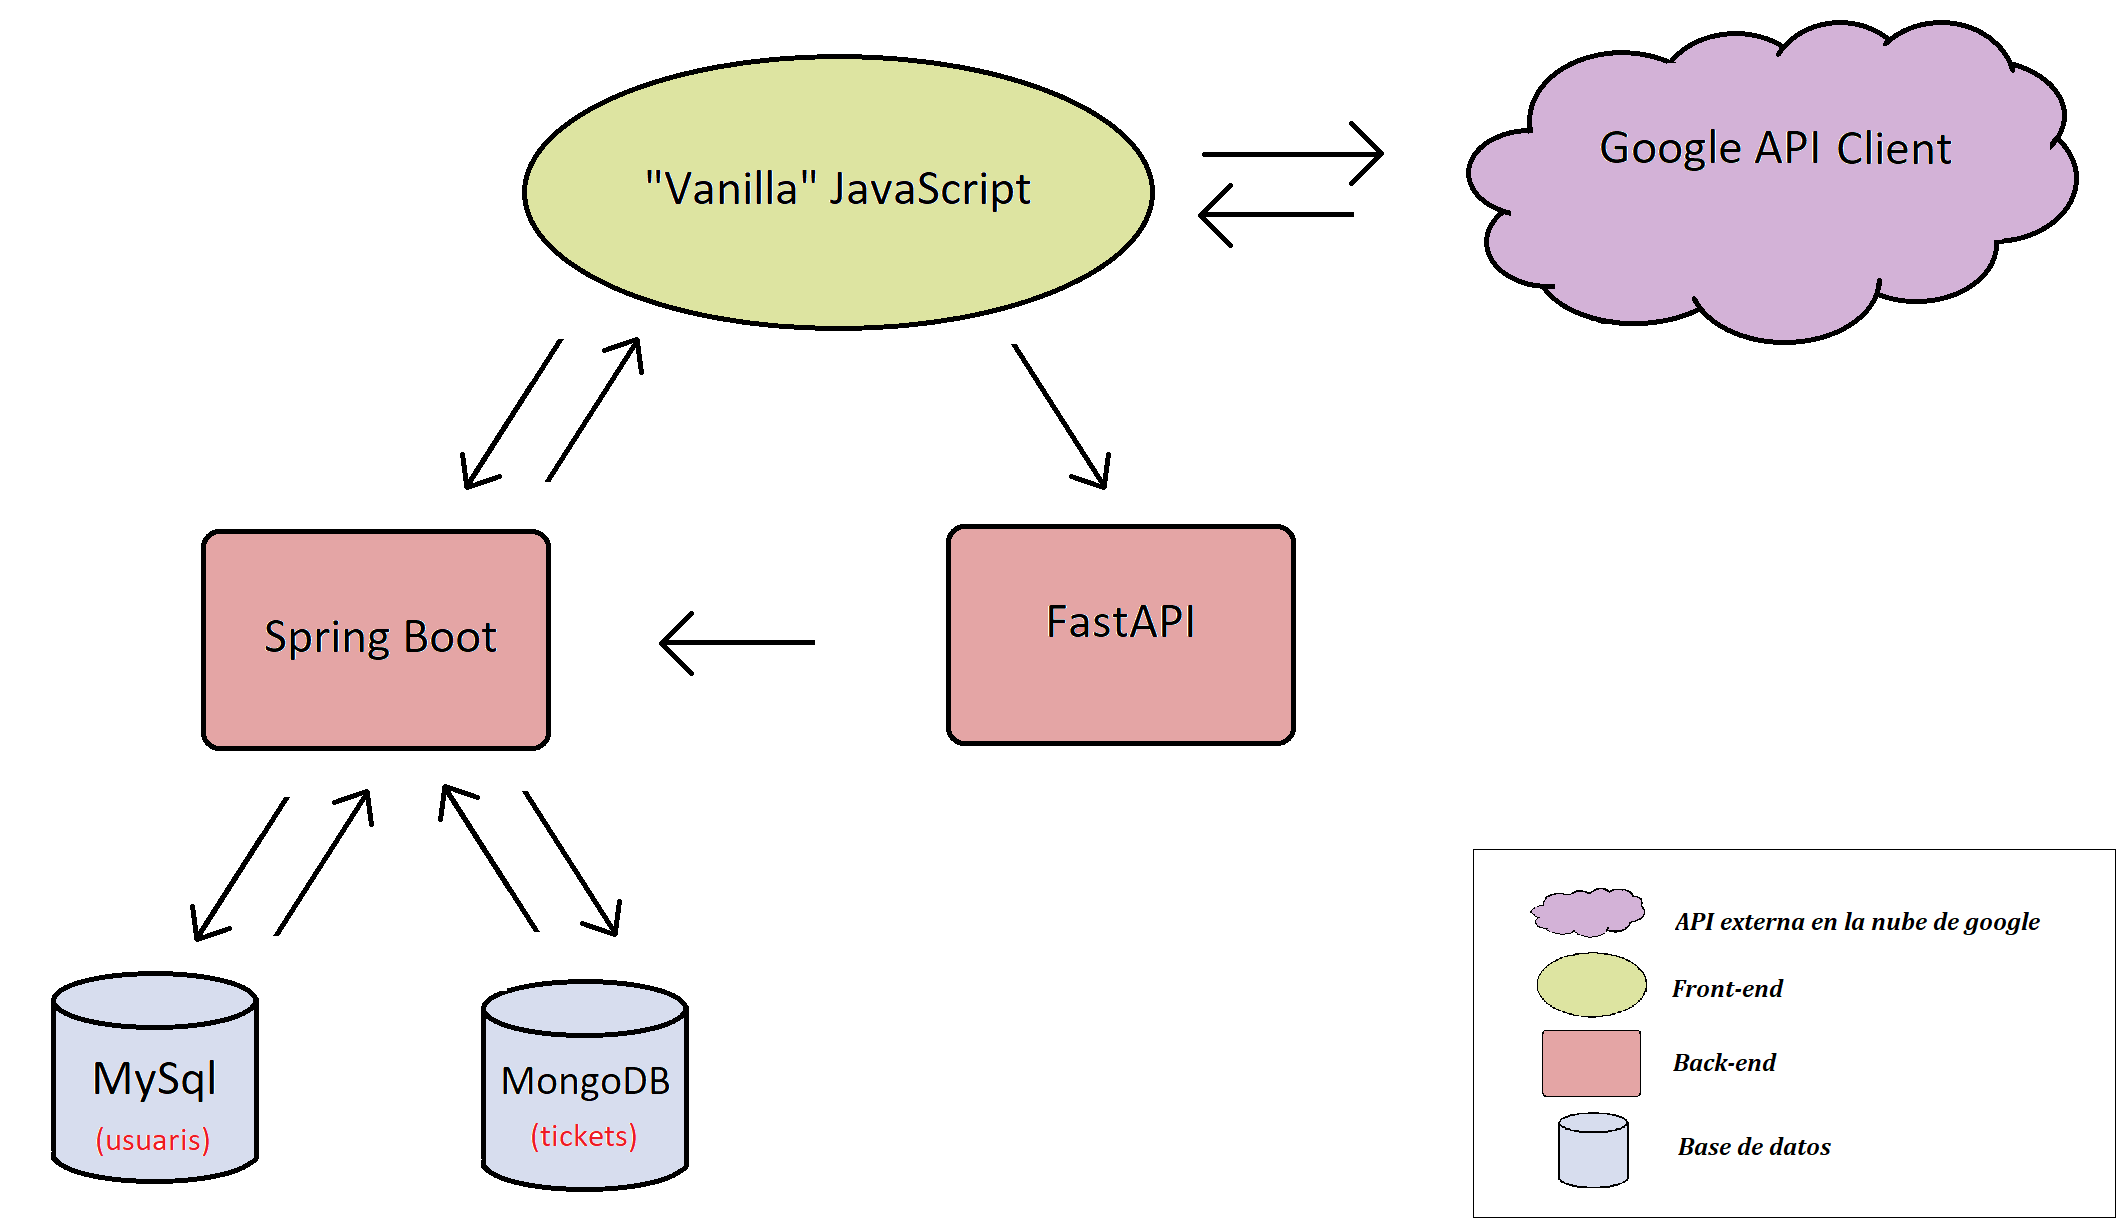
\includegraphics[width=1\textwidth]{img/diagramaSistemesAplicacioMercapp.png}
			\caption{Diagrama de sistemas de la aplicación mercApp. Tenemos el back-end principal (Spring Boot) donde se mandan a guardar y leer tanto los usuarios (mySql) como los tickets (MongoDB). El back-end secundario, con fastAPI, parsea los tickets y los pasa a formato estructurado JSON para hacer que Spring Boot lo persista en en MongoDB. Google API Client permite extracción de tickets del gmail del usuario. El front-end con "Vanilla" JavaScript muestra las vistas al usuario en función del token de acceso.}

			
			\label{fig:diagramaSistemesAplicacioMercapp} 
		\end{figure}
		\FloatBarrier
				
				
			\subsection{Camino durante registro de usuario}
				
				
				\setlength{\belowcaptionskip}{3pt}
				\FloatBarrier
				\begin{figure}[H]
					\centering
					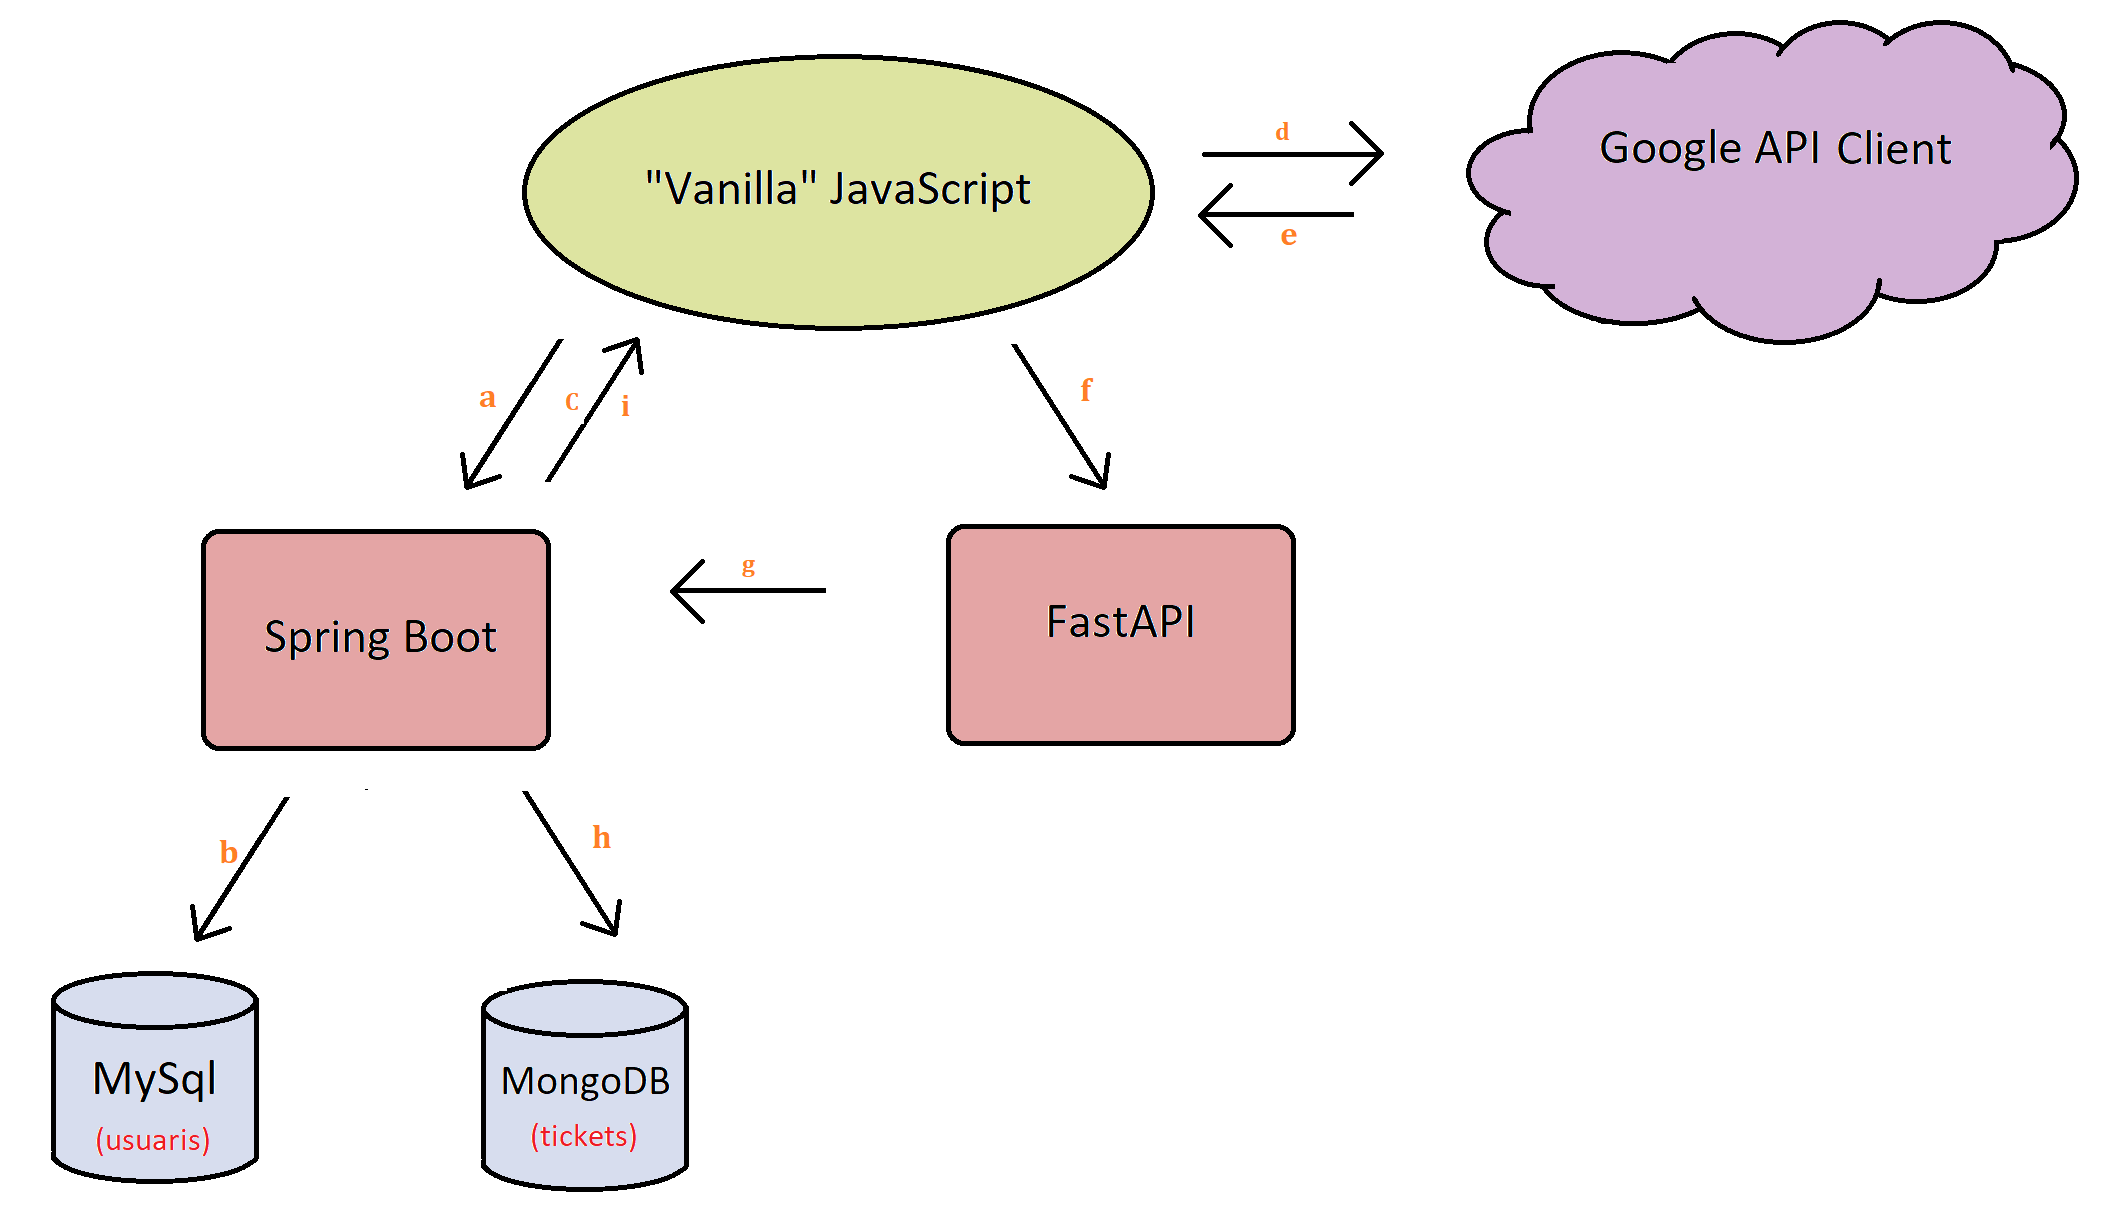
\includegraphics[width=1\textwidth]{img/diagramaSistemesAplicacioMercappCAMIREGISTRE.png}
					\caption{Simplificación de los caminos activados en el diagrama de sistemas durante el registro de un usuario, hasta que este tiene acceso al dashboard de visualización con éxito en todas las partes del proceso: a) Usuario pone correo y contraseña. b) guardamos correo y hash contraseña. c) Mandamos vista al usuario para que nos dé acceso a tickets digitales junto con token de acceso con permisos = 0. d) usuario se autentica con \textbf{google API client.} e) tickets regresan al navegador. f) fastAPI recoge los  tickets y los parsea a formato JSON estructurado. g) fastAPI delega en SpringBoot la persistencia de datos. h) la persistencia de los tickets se hace en MongoDB. i) Spring Boot manda token de acceso con permisos = 1 para que frontend muestre el análisis de los tikets en el dashboard.}
					\label{fig:diagramaSistemesAplicacioMercappCAMIREGISTRE} 
				\end{figure}
				\FloatBarrier
				
				
		\subsection{Camino durante inicio de sesión}
		
	\textbf{TO DO}
		
	
	\chapter{Desarrollo del proyecto} %OBLIGAT
	

	
	
				
			\section{GitHub del proyecto}
			
				Para desarrollar este proyecto se ha trabajado con GitHub y git. Dado que no ha habido trabajo en equipo no se han utilizado pull requests a la rama main sino simplemente se ha seguido la estrategia de crear ramas de característica y, una vez son satisfactorias, hacer un merge en la rama main en local.
				
				Un flujo de trabajo habitual es mediante ramas de característica (puede verse anexo \ref{sec:anexoFlujoGit}). También puede verse el GitHub del proyecto a continuación. Dentro del readme del proyecto encontraréis instrucciones para su descarga y clonado.
				
				Las instrucciones para correr los componentes del proyecto en sus respectivos entornos de desarrollo están en el apartado \ref{sec:entornosDesarrollo}. El despliegue de la aplicación mediante contenedores se encuentra explicado en \ref{sec:despliegue}.
			

			
			
			
			
				\textbf{Link al repositorio} $\rightarrow$ \href{https://github.com/blackcub3s/mercApp}{https://github.com/blackcub3s/mercApp} 
			
	
	
		
			\section{Entornos de desarrollo}
			\label{sec:entornosDesarrollo}
			
				Para el back-end de Java con SpringBoot se ha utilizado el editor Java \texttt{IntelliJ Idea community edition} que expone el backend en el puerto\textbf{ 8080}: se han utilizado extensiones necesarias para correr el proyecto que permiten sacar provecho de Lombok sin las cuales correr el proyecto en IntelliJ fallará\footnote{¡Para correr el proyecto back-end con\textit{ Spring Boot} abrir con intelliJ la carpeta app!}.
				
				Para el front-end (archivos estáticos: HTML, CSS y JavaScript) se ha utilizado \texttt{VScode}, con la extensión live server para poder hacer llamadas al back-end directamente desde el puerto \textbf{5500} \footnote{¡El proyecto \textit{front end} con \textit{vanilla javascript} debe abrirse con vscode en la carpeta \textbf{app} y ejecutarlo en live server, si no \textbf{no} funcionará correctamente!}.
				
				Para el back-end con fast-api se ha utilizado el servidor embedido en el propio framework, expuesto en el puerto \textbf{8000}.
				
				Para la base de datos mySQL se ha utilizado el editor mySQL workbench que corre en el puerto \textbf{3306}.
		
	
			\section{Despliegue}
			\label{sec:despliegue}
				Los componentes del apartado \ref{sec:entornosDesarrollo} de entornos  desarrollo se han \textit{dockerizado} de modo que cada uno de ellos sea un microservicio, a excepción (por ahora), de las bases de datos. Hemos sido cuidadosos de que los microservicios en Docker corran en los mismos puertos que los servidores embedidos con los que hemos hecho el desarrollo de la aplicación mercApp: por claridad y porque múltiples archivos dependen ya de ellos.
				
				Para crear la imagen de cada microservicio hemos creado un Dockerfile. Luego, para crear los contenedores y crear de nuevo las imágenes en caso que haya cambios en los archivos, para cada uno de estos microservicios, hay un script denominado \textit{creaImatge\_i\_arrancaContenidor.sh}\footnote{La explicación pormenorizada de sus comandos, para el caso de fastAPI por ejemplo, puede verse en el apartado TAL} que reunirá todos los subcomandos de docker necesarios para el ciclo de vida de su imagen (build), e instanciado de contenedor (create, start, stop, rm). Todo ello haciendo solamente: 
				
				\begin{lstlisting}[language=bash]
	bash creaImatge_i_arrancaContenidor.sh
				\end{lstlisting}
				
				
				
				
				
				Así, no tenemos que preocuparnos de parar el contenedor, borrarlo y luego crear la imagen (ver imagen \ref{fig:dockeritzacioAplicacioPlantilla}).
				
				
				\FloatBarrier
				\setlength{\belowcaptionskip}{3pt}
				\begin{figure}[H]
					\centering
					\caption{En rojo los archivos que crean una imagen y arrancan su contenedor, para cada microservicio.}
					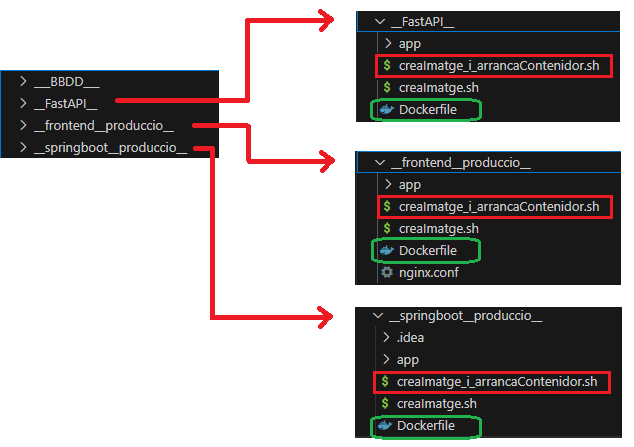
\includegraphics[width=.7\linewidth]{img/dockeritzacioAplicacioPlantilla.png}
					\label{fig:dockeritzacioAplicacioPlantilla}
				\end{figure}
				\FloatBarrier
				
			

			
			\section{Desarrollo back-end (Spring Boot)}
			\label{sec:parteSpringBoot}
			
				\subsection{Estructura de la aplicación}
				\label{sec:estructuraAplicacion}
				
				La parte de mercApp programada con Java (Spring Boot) se puede ver en el repositorio de GitHub del proyecto abriendo esta carpeta: \href{https://github.com/blackcub3s/mercApp/tree/main/APP%20WEB/__springboot__produccio__/app}{aquí} (eecomendamos al lector que abra y corra el proyecto con IntelliJ abriendo la carpeta mencionada del GitHub, pero en local). Se podrá ver entonces \textit{tres} rutas importantes (que son las tienen todos los proyectos Spring Boot):
				
				\vspace{-.9em}
				\begin{itemize}
					\setlength{\itemsep}{-.5em}
					\item \textbf{src/main/java} $\rightarrow$ En esta ruta encontramos los \textit{packages} y las clases del proyecto (ver figura \ref{fig:estrucutraAplicacioJAVARESOURCES} recuadro en \textcolor{red}{rojo}).
					\item \textbf{src/main/resources} $\rightarrow$ Dentro de esta carpeta  nos encontramos con el archivo \texttt{application.properties}. trata de un archivo de configuración donde se define, por ejemplo, el conexionado con la base de datos (ver figura \ref{fig:estrucutraAplicacioJAVARESOURCES} recuadro en \textcolor{green}{verde}) y logback-spring.xml que, aunque no está definido por defecto en una aplicación Spring Boot, si lo añadimos lo que hace es que los logs del proyecto se guarden en \textit{logs/spring.log} en lugar de salir a terminal\footnote{La ruta se crea automáticamente}. Aquí aparece como un \textit{.txt} en lugar de un \textit{.xml} porque por ahora no queremos que se guarden los errores.
					\item \textbf{pom.xml} $\rightarrow$ Es un arhivo donde encontramos el árbol de dependencias de Maven\footnote{Maven es una herramienta de automatización para la construcción de proyectos Java. Gestiona todas las dependencias, que se descargan desde un repositorio central muy vivo donde hay millones de nuevos paquetes publicados anualmente (\href{https://mvnrepository.com/repos/central}{ver link}). Maven permite empaquetar el proyecto en un .jar o .war fácilmente, entre otras cosas.} (ver figura \ref{fig:estrucutraAplicacioJAVARESOURCES}, recuadro en \textcolor{blue}{azul}): cada vez que añadimos una dependencia estamos añadiendo nuevas funcionalidades a nuestro proyecto SpringBoot a través de una descarga automatizada del repositorio central de Maven.
					
					
				\end{itemize}
				
				
				\setlength{\belowcaptionskip}{3pt}
				\FloatBarrier
				\begin{figure}[H]
					\centering
					\caption{Estructura del back-end de Spring Boot en la aplicación mercApp. \\ {\footnotesize (Cajas de color $\rightarrow$ $\{$\textcolor{red}{clases del proyecto}, \textcolor{green}{archivos de configuración}, \textcolor{blue}{dependencias de Maven}$\}$) }}
					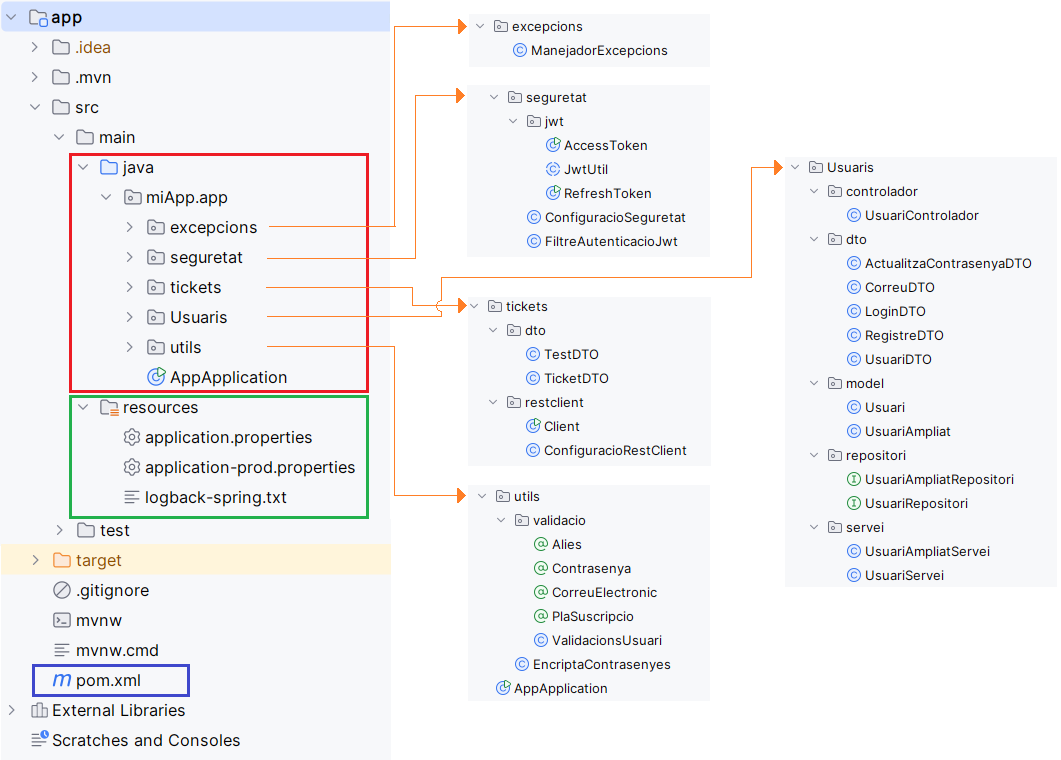
\includegraphics[width=1\textwidth]{img/estrucutraAplicacioJAVARESOURCES_final_rallat.png}
					
					\label{fig:estrucutraAplicacioJAVARESOURCES} 
				\end{figure}
				\FloatBarrier
				
				

				

				\subsubsection{src/main/java: las clases del proyecto}
				
				
				Dentro de \textbf{src/main/java} tenemos la ruta \textbf{miApp.app/utils/validacio}	donde residen las clases de anotación utilizadas para permitir que los campos de formulario de entrada se validen en el back-end (nótese que, con esto, hemos establecido redundancia de validaciones por si se diese el caso que un usuario maliciosamente intentase hacer llamadas directas a la API, esquivando así las validaciones ya definidas en el front-end): los archivos y su explicación quedan referenciados en detalle en el apartado \ref{sec:validacioDadesBACK}.
				
				
				
				Dentro de \textbf{src/main/java} tenemos también la ruta \textbf{miApp.app/seguretat/jwt} donde tenemos clases que generan tokens de acceso y de refresco  a partir de una clave secreta que solo está en el servidor, que referenciamos en detalle dentro de \ref{sec:implementacionJWTjava}; Análogamente, las clases que permiten implementar la autenticación y la autorización a partir de los tokens generados por las clases anteriores, las referenciamos también en detalle dentro de \ref{sec:classesSecuritzacioClaimsIfirma}.
				
				Dentro de \textbf{src/main/java} tenemos también la ruta \textbf{miApp.app/seguretat} encontramos la clase \textit{EncriptaContrasenyes.java}, que utilizamos en el servicio de usuaris para hashear las contraseñas en la base de datos. Esto lo explicamos en detalle dentro de \ref{sec:implementacioHashContra}.
				
				
				TO DO EXPLICAR 	\hspace{3em} usuari, repository, service, controller de 
			
				TO DO EXPLICAR 	\hspace{3em} classes per a fer la unio amb el backend de fast API mitjançant restClient.
				
				
				
				\subsubsection{src/main/resources: archivos de configuración}
				
				TO DO EXPLICAR application.properties
				
				\subsubsection{pom.xml: dependencias de maven}
				
				
				 
				
				TO DO EXPICAR pom.xml: parlar de la versio i link a la pagina on la versio.
				
				
			
				
				\subsection{Autenticación y Autorización}
				
				\subsubsection{método utilizado: JWT}
				
				Para autenticar y autorizar a los usuarios no utilizaremos sesiones. Las sesiones, tal y como vimos en la asignatura de desarrollo web entorno servidor, requieren guardar un estado en el servidor (si tenemos 100 usuarios conectados necesitamos rastrear 100 personas en el servidor) y un identificador de sesión en una cookie segura con HttpOnly puesto a True guardada en el navegador de cada uno de los usuarios conectados que lo identifica en relación al servidor.
				
				Sin embargo, existe un método de acceso por token más escalable que no requiere guardar sesiones en el servidor (es decir, es un método ``stateless'' o sin estado) con el que nos basta tener solamente la Cookie Segura para guardarlo y ya está. Es un token que está autocontenido: es decir, puede contener ya el ID de usuario, nombre de usuario, roles que luego permitirán dar permisos o no en el servidor para acceder a determinadas APIs o recursos, etc. En definitiva, con JWT tenemos una autenticación más eficiente y un control del acceso preciso (autorización) sin necesidad de almacenar sesiones en el servidor.
				
				
				A este sistema lo llamamos JSON Web Token (\texttt{JWT}) y toda la información que contiene está \textbf{firmada digitalmente} con SHA256 mediante una clave privada (el ``secret'') que solo tenemos nosotros en el servidor\footnote{El token está firmado, pero no cifrado: todo el mundo puede ver su contenido.}. Esta clave es igual para todos los tokens que generemos: la firma digital que emana de esta clave estará embedida, por así decirlo, en cada uno de esos tokens y \textit{será inválida} si un atacante ha modificado el token y nos lo devuelve al servidor tratando de suplantar la identidad de algún usuario; con ello, el servidor rechazará la integridad del token y evitará que pueda acceder a recursos del usuario al que trata de suplantar.
				
				JWT no es perfecto, por supuesto. Una desventaja del JWT es que una vez puesta una fecha de expiración el desarrollador ya no la puede cambiar. En las sesiones del servidor se pueden extender las sesiones si se detecta actividad del usuario, acortarlas si pasa justo lo contrario o incluso cerrar la sesión de un usuario en remoto; pero con JWT no es posible: una vez creado el Token de acceso la fecha de actividad del mismo no se puede modificar (¡porque no puedes invalidar un token ya existente!), lo cual permite que simplemente un atacante robe el token de acceso sin modificarlo y lo use hasta su fecha de expiración.
				
				Se proponen dos soluciones posibles a este problema, ninguna de las cuales ha sido implementada en este proyecto y queda definitivamente como uno de los puntos de mejora:
				
				\begin{itemize}
					\setlength{\itemsep}{.0em}
				
					\item 1. Tener dos tokens almacenados en el cliente: el ``access token'' que es el que permite autenticar y autorizar, del que hemos hablado hasta ahora; y otro token denominado ``refresh token'', que se utiliza
					para obtener un nuevo token de acceso cuando el token de acceso actual expire, o para obtener tokens de acceso adicionales con un alcance idéntico o más limitado -es decir, duración más corta- \cite{stackoverflow_refreshTokenAvantatjaSeguretat}
					
					\item 2. Crear una black-list de tokens de acceso donde se añadirán los usuarios que hayan hecho ``log out'' ANTES de la expiración programada de su token de acceso: así si un token de acceso todavía no expirado sabemos que su usuario se ha deslogueado, en caso que sea robado, el servidor rechazará la petición no permitiendo acceso a recursos \cite{stackOverflow_blackList}).
 
					
				\end{itemize}

				
				
				En este trabajo solo utilizaremos ``access tokens'' y ya está. Cuando un usuario se desloguee, lo que haremos simplemente será borrar el access token del local storage. Tampoco guardaremos los tokens en una cookie segura porque complica el desarrollo (de nuevo, otro punto a mejorar a futuro en este proyecto).
			
				 
				 \noindent En resumen, \texttt{las ventajas} que tiene JWT vs uso de sesiones (si asumiéramos que tanto el JWT como el SESSID se guardasen en una cookie segura, respectivamente) serían las siguientes:
				 
					\begin{tabular}{l}
						\textbf{- No depende del almacenamiento en el servidor} \\
						\textbf{- Firmado digitalmente} \\
						\textbf{- Mayor control sobre el acceso} \\
						\textbf{- Mayor descentralización} \\
						\textbf{- Menos carga para el servidor}
					\end{tabular}
									 
				   \noindent Y la \texttt{desventaja} más evidente que tiene JWT, es, en nuestra opinión, su complejidad\footnote{Se puede ver una tabla de diferencias más en profunidad, especialmente en materia de seguridad en el anexo \ref{sec:anexo_JWTvsSESSIONS})}, pues para tener un buen equilibrio entre facilidad de uso y seguridad es necesario almacenar los tokens en el cliente para conseguir que uno se renueve (el token de aceso y el de refresco, como comentamos):
				  
				  \begin{tabular}{l}
					 \textbf{- Caducidad de tokens irrevocable}\\
					 \textbf{- Renovación de tokens de acceso con uno de refresco}
				  \end{tabular}
				 

				
				
				
				\subsubsection{¿Qué compone un JWT?}
				\label{sec:queComponeJWTbackend}
				
				\noindent El JWT se compone de tres partes separadas por \textit{puntos}: \textbf{el header}, \textbf{el payload} y \textbf{la signatura}. En la página \href{https://jwt.io/}{https://jwt.io/}, como veremos después, se puede ver si los tokens son válidos, observar el contenido de su payload, etc. \cite{jwtio}. A saber:
				

				\begin{itemize}
					\setlength{\itemsep}{-.5em}
					\item 				\textbf{Los headers}: Aportan información sobre el algoritmo que lo encriptó.
					\item 				\textbf{El payload}: Es donde está la información que nos interesa del token: el sujeto que lo generó (``sub''), el momento en que se generó el toquen (``iat'', o ``issued at'') y la fecha de expiración (``exp'' o ``expiration time''). También podemos tener ahí otros pares clave valor que podremos querer definir, por ejemplo, que contengan el id del usuario y sus roles o permisos que son los que nos permitirán dejar que un determinado usuario pueda consultar o no ciertos recursos.
					
					\item \textbf{La signatura}: Es la parte que garantiza la integridad del token y evita que sea alterado por terceros. Se genera aplicando un algoritmo de hash (en nuestro caso el SHA256) a la combinación del header y el payload, junto con la clave secreta que solo conoce el servidor (es lo que permetirá al servidor rechazar el token si no es válido -i.e. ha sido manipulado).
				\end{itemize}
				
				Podéis observar estas tres partes en colores en la figura \ref{fig:jwtioMostraPayload} que veremos después.
				
				
				

				

				
				
				\subsubsection{Implementación de JWT en java SpringBoot}
				\label{sec:implementacionJWTjava}
				Para poder implementarlo añadimos la dependencia \textbf{jjwt} en \texttt{pom.xml} que es la que nos permite definirlo.
				
				
				\begin{lstlisting}[language=XML, basicstyle=\ttfamily\small, keywordstyle=\color{red}]
					
	<dependency>
		<groupId>io.jsonwebtoken</groupId>
		<artifactId>jjwt</artifactId>
		<version>0.12.6</version>
	</dependency>
					
				\end{lstlisting}
				
				
		En el proyecto se han creado tres clases dentro de sus respectivos archivos en la ruta \texttt{src/main/java/} \texttt{miApp.app/seguretat/jwt} denominadas:
		
		\begin{itemize}
			\setlength{\itemsep}{-.4em}
			\item \textbf{JwtUtil}
			\item \textbf{AccessToken}
			\item \textbf{RefreshToken}
		\end{itemize}
		  
		
		En la clase \textbf{JwtUtil} hemos creado un método que obtiene las \textit{claims} (pares clave valor que contienen la carga útil de un JWT) y en el constructor hemos creado la definición de una clave privada con la que derivar todas las instancias que hagamos de esa clase -es decir, todos los tokens que se cifren con esa contraseña-. De esta clase hemos heretado las otras dos: La subclase que nos genera el \textit{token de acceso}, \textbf{AccessToken}; y la que nos genera el \textit{token de refresco}, \textbf{RefreshToken}. A continuacion podéis, de estas tres, la más importante (la clase RefreshToken la hemos programado para usarla a futuro pero no se ha utilizado para la implementación del sistema de autenticación y autorización en este proyecto): 
		
		

		
\begin{lstlisting}[language=Java, basicstyle=\ttfamily\footnotesize, keywordstyle=\color{magenta}]
				
@Component
public class AccessToken extends JwtUtil {
	
  private static int tExpM; //minuts per a exprirar el token
	
  public AccessToken() {this.tExpM = 10;}
	
  //FINALITAT: Generar un JWT d'acces.
  public String genera(String correu, int idUsuari, byte permisos) {
	Map<String, Object> dadesExtraApayload = new HashMap<>();
	dadesExtraApayload.put("permisos", permisos);
	dadesExtraApayload.put("idUsuari", idUsuari);
		
	return Jwts.builder()
	 .setClaims(dadesExtraApayload) //dades customitzades
	 .setSubject(correu)            //guardo nom subjecte (clau "sub")
	 .setIssuedAt(new Date())       //data creacio (clau "iat" payload)
	 .setExpiration(new Date(System.currentTimeMillis() + (tExpM*60*1000)))
	 .signWith(SignatureAlgorithm.HS256, clauSecreta.getBytes())
	 .compact();
}


\end{lstlisting}
		
		
		
		Con la función \textbf{genera()} de la clase AccessToken arriba mostrada, y con los parámetros necesarios que serán necesarios para autorizar (idUsuari) y autenticar (permisos), podemos generar un token de acceso en ``accesJWT'' que es el que usamos en la aplicación para permitir acceder a los endpoints o no:
		
		
		
\begin{lstlisting}[language=Java, basicstyle=\ttfamily\footnotesize, keywordstyle=\color{magenta}]

AccessToken accessToken = new AccessToken();
String accesJWT = accessToken.genera(
	"santo@gmail.com",  //campoSub
	2, //idUsuari
	1  //permisos
);


\end{lstlisting}
		
		Si vemos la figura \ref{fig:jwtioMostraPayload} que tenemos a continuación, veremos en la mitad izquierda un token de acceso generado por la función anterior. Fijémonos que internamente ese token está estructurado en las tres partes de la parte derecha de la imagen, siendo la payload la más importante:
		
	
			\setlength{\belowcaptionskip}{3pt}
			\FloatBarrier
			\begin{figure}[H]
				\centering
				\caption{Decodificación mediante \href{https://www.jwt.io}{jwt.io} de un token de acceso usado en nuestra aplicación generado con la función ``genera()'' de la clase AccessToken. La Payload con las claims en flecha verde.}
				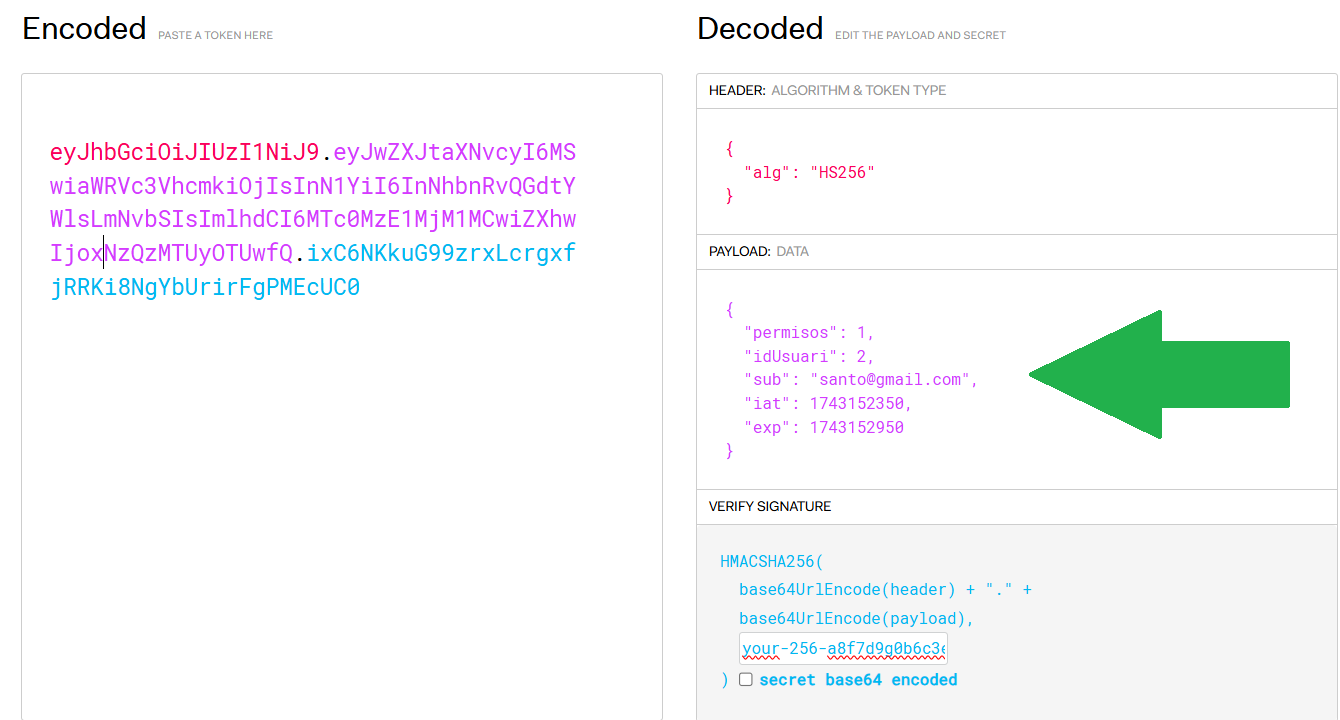
\includegraphics[width=1\textwidth]{img/jwtio_mostra_payload.png}

				\label{fig:jwtioMostraPayload} 
			\end{figure}
			\FloatBarrier

		
\begin{lstlisting}[language=Java, basicstyle=\ttfamily\footnotesize, keywordstyle=\color{magenta}]
			
		
		{
		    "permisos": 1,
		    "idUsuari": 2,
		    "sub": "santo@gmail.com",
		    "iat": 1743152350,
		    "exp": 1743152950
		}
			
\end{lstlisting}
		
		
		
		
		
		Al generar las tres clases hemos utilizado herencia porque la clave privada es la misma para ambos tipos de token (tanto el de acceso como el de refresco), mientras que los métodos para generar cada uno de los dos tipos de token cambian. En StackOverflow existe un debate para ver si hay que tener una clave privada distinta para cada tipo de token, por si el lector está interesado \cite{stackoverflow_jwt_refresh_token_secret}. Después de ver la entrada en stackOverflow Se ha optado por compartir claves para ambos tipos.
		
		
		En la clase \textbf{JwtUtil} tenemos una función denominada \texttt{getClaims()} que es la que utilizaremos en el Service de nuestra aplicación para poder autenticar y autorizar usuarios. Las tres clases pueden ser consultadas en el anexo \ref{sec:anexoCreacionYverificacionJWT} o en el GitHub del proyecto (\href{https://github.com/blackcub3s/mercApp/blob/main/APP%20WEB/__springboot__produccio__/app/src/main/java/miApp/app/seguretat/jwt}{link})\footnote{Se recomienda encarecidamente al lector optar por esta última opción}\footnote{Al poner las tres clases en anexo se omitieron las funciones main donde se testeaban las funciones de creación de tokens con control de excepciones, comentarios e imports por falta de espacio en el DIN A4.}.
		
		\subsubsection{Enviar por primera vez el Access Token hacia el front-end (registro)}
		\label{sec:enviarPorPrimeraVezAccesTokenDESDEBACKEND}
		
		Cuando el usuario consigue poner la contraseña correcta en la página de registro del front-end (\texttt{pas3C\_crearContrasenya.html}), esta contraseña se manda conjuntamente con el correo electrónico\footnote{el correo electrónico  lo teníamos guardado en el localStorage de la página de registro inicial.}  mediante una petición POST al controlador de endpoint \textit{api/registraUsuari} de nuestro back-end de springboot. Este controlador responde entonces mandando de vuelta al cliente \textbf{el token de acceso}, que se \textbf{guardará} en el localStorage del navegador del usuario.
		
		
		Así las cosas, podemos testear que esto funciona como es debido haciendo una solicitud POST con la aplicación Postman\cite{postman_api_platform} al endpoint \textit{api/registraUsuari} con un correo que no esté guardado en la tabla usuaris: por ejemplo, ``nuevoUsuario@gmail.com''; y con una contraseña válida para ser guardada de acuerdo con nuestro requisitos de seguridad\footnote{Mínimo 8 caracteres, una minúscula y una mayúscula y sin caracteres peligrosos.}: si todo va bien deberemos obtener la figura \ref{fig:detallPostmanRegistraUsuari}:
		
		
		
		\setlength{\abovecaptionskip}{0pt}
		\FloatBarrier
		\begin{figure}[H]
			\centering
			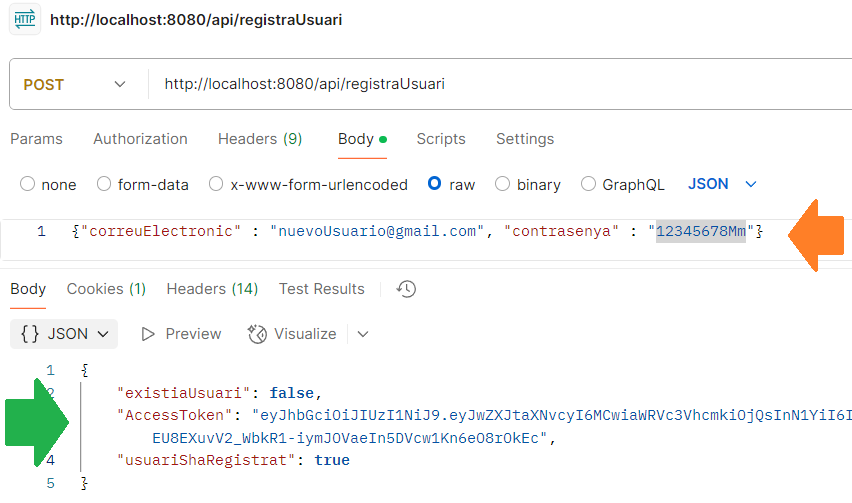
\includegraphics[width=1\textwidth]{img/detallPostmanRegistraUsuari.png}
			\caption{Creación de un nuevo usuario llamando con una solicitud POST al endpoint ``api/registraUsuari'' cuando las validaciones del objeto RegistreDTO del back-end lo permite. En naranja se muestra el body de la petición (lo que el cliente envía al servidor) y en verde el body de la respuesta (lo que el servidor devuelve al cliente).}
			
			\label{fig:detallPostmanRegistraUsuari} 
		\end{figure}
		\FloatBarrier
		
		
		Tenemos otro endpoint que también expide tokens de acceso, mucho más habitualmente que el anterior: es el endpoint que se consume cuando iniciamos sesión, en \texttt{pas2C\_login.html}: el endpoint ubicado en la URI\footnote{Uniform Resource Identifier} \textit{/api/login}. Si intentamos iniciar sesión con un usuario ya existente en la tabla de usuarios obtendremos algo como esto:
		
		\setlength{\abovecaptionskip}{0pt}
		\FloatBarrier
		\begin{figure}[H]
			\centering
			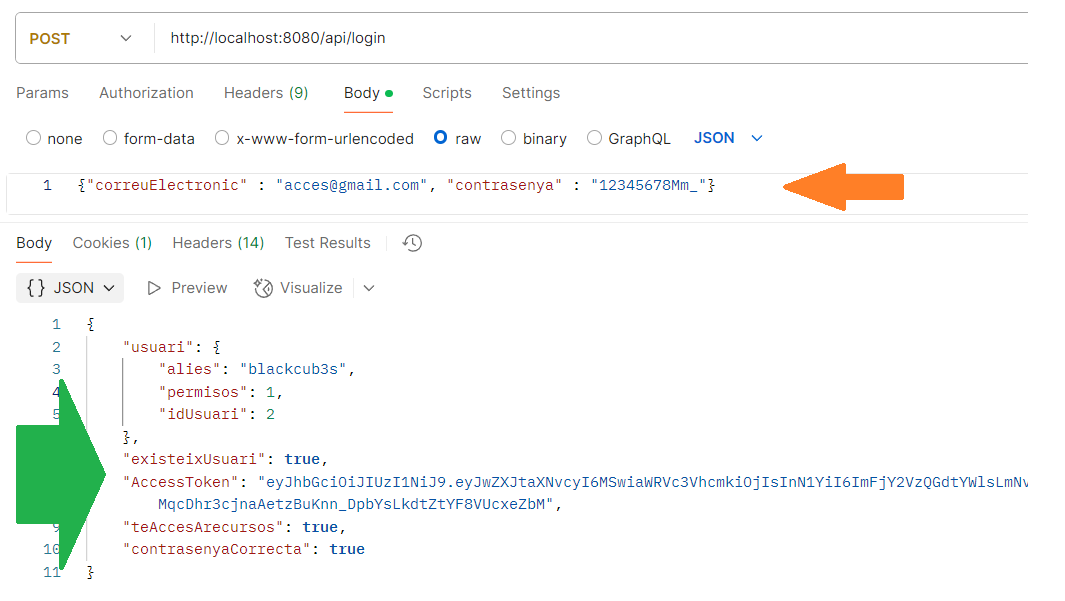
\includegraphics[width=1\textwidth]{img/detallPostmanLogin.png}
			\caption{Iniciando sesión con un usuario ya existente mediante ``api/login'' mandando los datos de ``correuElectronic'' y ``contrasenya'' que leerá y validará el LoginDTO del back-end. En naranja es el body de la petición y en verde el body de la respuesta.}
			
			\label{fig:detallPostmanLogin} 
		\end{figure}
		\FloatBarrier
		
		\textbf{POTSER POSAR LES FUNCIONS DEL CONTROLADOR I DEL SERVICE QUE HO FAN ENLLAÇANT CODIS DE GITHUB.}
		
		La parte de recepción del token en el front-end y de su manejo podéis encontrarla en el apartado \ref{sec:recibirAccesTokenENFRONTEND}

		
		
		
		
		
		
	
		
		\subsubsection{Recibir en el back-end el JWT enviado desde el front-end y con él securizar un endpoint de la API mediante interpretación de claims y verificación de firma.}
		\label{sec:classesSecuritzacioClaimsIfirma}
		
		Después de crear las tres clases en Java de las que hemos hablado en el apartado \ref{sec:implementacionJWTjava} anterior y haber mandado el token de acceso al front mediante el body de las \textit{responses} a los endpoints \textit{api/registraUsuari} o \textit{api/login}, podemos empezar a 
		implementar la protección de endpoints con JWT. 
		
		Asumamos que nos llega al back-end un token de acceso en una solicitud HTTP de un usuario que ya ha recibido su token y quiere ahora acceder al dashboard de visualización (a través de la heather ``Authorization''). 
		
	\textbf{	POSA EL CAS REAL QUAN L'HAGIS PROGRAMAT QUE AQUEST ENDPOINT ENCARA NO EXISTEIX}: La solicitud HTTP con el susodicho token se hace via GET a (\texttt{'usuaris/{id}/tiketsVERIFICARSIEXISTEIX'}) (ver subseccion \ref{sec:estructuraAplicacion}, en ControladorUsuari.java). 
		
		En javascript puro, desde el cliente, esta solicitud HTTP la pondríamos conseguir de la función fetch(), poniéndole uno de los pares clave valor con el inicio ``Bearer'' (por convenio) tal que así:
		
				
\begin{lstlisting}[language=Java, basicstyle=\ttfamily\footnotesize, keywordstyle=\color{magenta}]

fetch("'http://localhost:8080/usuaris/{id}/endpointTikets'", {
	method: "GET",
	headers: {
		"Content-Type": "application/json",
		"Authorization": "Bearer "+tokenJWT;
	},
	...
}
\end{lstlisting}
		
		 Queremos conseguir que ese endpoint permita en cada solicitud \textbf{Autenticarlo}, es decir, determinar que dice ser quien es mediante el hecho de encontrar en el token verificado su \textcolor{red}{idUsuari} correspondiente (y acceder a la información de sus tickets); y a su vez \textbf{Autorizarlo}, es decir, dar acceso a ese usuario a los recursos a los que se le permita acceso mediante la variable \textcolor{orange}{permisos} correspondiente.
		
		 Estos dos pasos irán en función del valor de la variable que haya emanado de la base de datos al conceder el token mediante \textcolor{red}{idUsuari} para el caso de la \textbf{Autenticación} -ver \href{https://github.com/blackcub3s/mercApp/blob/b01cec515bb9af27a1faa24258abb4313ef275cd/APP%20WEB/__springboot__produccio__/app/src/main/java/miApp/app/Usuaris/model/Usuari.java#L30}{linea github}-, y de la variable \textcolor{orange}{permisos} del model de la @Entity class Usuari - ver \href{https://github.com/blackcub3s/mercApp/blob/b01cec515bb9af27a1faa24258abb4313ef275cd/APP%20WEB/__springboot__produccio__/app/src/main/java/miApp/app/Usuaris/model/Usuari.java#L42}{linea github}- para el caso de la \textbf{autorización}). Para ello hay \textbf{tres} pasos que debemos implementar dentro del back-end de SpringBoot:
		
		
		
		
		\begin{itemize} 
			\setlength{\itemsep}{-1.5em}
			\item \textbf{PASO 1:} Extraer la información del usuario autenticado desde \textit{el payload} del token JWT entrante. Para ello crearemos un \textbf{Filtro de Autenticacion} dentro de \texttt{FiltreAutenticacio.java}\\
			\item \textbf{PASO 2:} Configurar el contexto de seguridad para que Spring Security reconozca los permisos, dentro de  \texttt{ConfiguracioSeguretat.java}. \\ 	
			\item \textbf{PASO 3:} Aplicar restricciones con \textbf{@PreAuthorize} en cada \textit{endpoint} que queramos proteger en el controlador, dentro \texttt{UsuariControlador.java}
		\end{itemize}
		

		\noindent \textbf{PASO 1: Extracción del payload (\textit{FiltreAutenticació.java})}
		\hrule
		\vspace{1em}
		
		Esta parte del código está llena de boilerplate. La clase \textit{FiltreAuntenticacioJwt.java} extiende de OncePerRequestFilter \cite{oncePerRequestFilter}, que como dice el propio nombre de la clase implementa un filtro que se desarrollará una y solo una vez por cada petición al servidor.
		
		Lo que hay que hacer aquí es implementar el método \textit{doFilterInternal()} donde colocamos la lógica específica del filtro. Se puede consultar este archivo en github del proyecto \href{https://github.com/blackcub3s/mercApp/blob/main/APP%20WEB/__springboot__produccio__/app/src/main/java/miApp/app/seguretat/FiltreAutenticacioJwt.java}{FiltreAuntenticacioJwt.java}
		
		Lo primero que hay que tener en cuenta al diseñar esta clase es que tenemos que hacer una inyección de dependencias: debemos incluir la clase que hemos diseñado AccessToken para implementar el token de acceso. Lo haremos simplemente incluyéndola en el constructor como un parámetro.
		
		Lo segundo que hay que considerar es la extracción del payload del token (donde tenemos la información que nos permitirá autorizar y autenticar). Para encontrar el token se hace de la \textbf{cabecera} ``Authorization'' de la solicitud HTTP entrante del front-end. La clave es ``Authorization'' y el valor asociado es, por convenio, un String ``Bearer '' concatenado al token de interés; algo así:
		

		
		\FloatBarrier
		\begin{table}[h]
				\centering
 				\textit{``Authorization'' : ``Bearer OJALWQ03P1WNOEGBO...''}
		\end{table}
		\FloatBarrier
		

		 
		  La programación necesaria para conseguir lo mencionado en el párrafo anterior queda recogida en este rango de lineas de GitHub (\href{https://github.com/blackcub3s/mercApp/blob/89efcf854d8bbab2addde3f7e817eb97f7737b95/APP%20WEB/__springboot__produccio__/app/src/main/java/miApp/app/seguretat/FiltreAutenticacioJwt.java#L33-L43}{ver rango}). 
		  
		  Luego una vez tenemos el token dentro de Spring Boot tratamos de sacar las Claims del Payload, es decir, la carga útil del token (\href{https://github.com/blackcub3s/mercApp/blob/89efcf854d8bbab2addde3f7e817eb97f7737b95/APP%20WEB/__springboot__produccio__/app/src/main/java/miApp/app/seguretat/FiltreAutenticacioJwt.java#L50-L54}{ver rango}). Y con ello ya podemos asignar tres roles a partir de la variable permisos del payload: 0, 1 o 2. 
		  
		  0 en la variable permisos de la tabla usuaris de mysql se asigna cuando un usuario ya se ha registrado dando correo y contraseña, pero no ha dado acceso a tickets digitales todavía; 1 en la variable permisos se da cuando el usuario en cuestión ya tiene acceso a la consulta del dashboard de la aplicación (ya se ha registrado y, \textit{además}, concedido acceso a tickets digitales); y 2 se da cuando el usuario en cuestión es superusuario y tiene acceso a consultar todos los recursos de la aplicación, tickets de los demás usuarios, etc. (\href{https://github.com/blackcub3s/mercApp/blob/89efcf854d8bbab2addde3f7e817eb97f7737b95/APP%20WEB/__springboot__produccio__/app/src/main/java/miApp/app/seguretat/FiltreAutenticacioJwt.java#L56-L66}{ver rango}). En definitiva, lo que estamos mencionando (por si el lector se imprimió la memoria y no tiene acceso directo al link de GitHub) las líneas relevantes del código que permiten esa asignación son estas:
		  
		  
		  
		  \begin{lstlisting}[language=Java, basicstyle=\ttfamily\footnotesize, keywordstyle=\color{magenta}]
		  
	Claims claims = accessToken.getClaims(token);
	
	
	Integer permisos = (Integer) claims.get("permisos"); 
	Integer idUsuari = (Integer) claims.get("idUsuari"); 
	
	// Creo autoritat basada en permisos
	String role;
	if (permisos == 2) {
	  	role = "ROLE_ADMIN";
	} else if (permisos == 1) {
	  	role = "ROLE_USER";
	} else {
	  	role = null;
	}
		  
		  \end{lstlisting}
		  
		  Importante es mencionar que en el fragmento de código anterior, al llamar al método $getClaims(token)$  se lanzará una excepción de tipo \textit{ExpiredJwtException} en caso que el token haya expirado, que recogeremos en el primer bloque Catch; y si el token está manipulado y no es válido, entonces se lanzará otra excepción que se recogerá en el segundo bloque Catch. Todo ello se informará como una response al cliente (\href{https://github.com/blackcub3s/mercApp/blob/89efcf854d8bbab2addde3f7e817eb97f7737b95/APP%20WEB/__springboot__produccio__/app/src/main/java/miApp/app/seguretat/FiltreAutenticacioJwt.java#L96-L115}{ver rango de líneas de código}).
		  
		  
		  Y finalmente hay que crear un objeto de tipo \textit{UsernamePasswordAuthenticationToken} ya definido dentro de SpringBoot. Su constructor permitirá tres parámetros: 
		 
		 	\begin{itemize}
		 	\setlength{\itemsep}{-.5em}

			  \item \textbf{el principal}, el primero, al que le pasaremos el \textcolor{red}{idUsuari}
			 \item  \textbf{credentials}, el segundo, que lo dejamos a null porque en JWT no se debe manejar credenciales ya que están contenidas dentro del token. 
			  \item \textbf{una collection con el role}, el tercero, que contendrá los roles que definimos antes. 
		  \end{itemize}
		  Este constructor nos permitirá restringir permisos para las APIs según el \textcolor{red}{idUsuari} al que esté vinculado su login (autenticación) y también según el valor de \textcolor{orange}{permisos} que tenga (autorización)\footnote{Cuidado! Lo cierto es que deben considerarse ambos parámetros a la vez en el controlador, como veremos en el paso 3. No es suficiente añadir roles a un determinado id. Solamente con los roles, Spring Boot no nos dejará, por ejemplo, que en una API que toma el idUsuari como parámetro en la URL (como la de este ejemplo) se pueda restringir a ese usuario específico para que no consulte los recursos de los demás usuarios con idUsuari distintos.}.
		  

		  
		  
 \begin{lstlisting}[language=Java, basicstyle=\ttfamily\footnotesize, keywordstyle=\color{magenta}]
	  	
UsernamePasswordAuthenticationToken authentication = 
new UsernamePasswordAuthenticationToken(
	idUsuari,
	null,
	Collections.singletonList(new SimpleGrantedAuthority(role))
);



 \end{lstlisting}
Este objeto \textit{authentication} que acabamos de crear entonces tenemos que guardarlo DENTRO del SecurityContextHolder:

		 
 \begin{lstlisting}[language=Java, basicstyle=\ttfamily\footnotesize, keywordstyle=\color{magenta}]

 SecurityContextHolder.getContext().setAuthentication(authentication)
	
\end{lstlisting}
	
	
	


		\noindent \textbf{PASO 2: Configuración contexto de seguridad (\textit{ConfiguracioSeguretat.java})}
		\hrule
		\vspace{1em}
		
		Sin esta clase, al añadir la dependencia de seguridad ``spring-boot-starter-security'' en \texttt{pom.xml} cualquier llamada a cualquier API va a devolver un código de error 401. Esto pasa porque al añadir la dependencia de seguridad mencionada nos encontramos con que se precisan ciertas configuraciones. La tres cosas que hay que hacer en la clase \textit{ConfiguracioSeguretat.java} para llevar a término las mencionadas configuraciones son:
		
		
		\begin{itemize}
		\setlength{\itemsep}{-.3em}
		 
		 
		\item \textbf{1. Inyectar jwtAuthenticationFilter}, una instancia de \textit{FiltreAutenticacioJwt.java}, a través del constructor para que actúe como dependencia.
		 
		\item \textbf{2. Especificar que jwtAuthenticationFilter va ANTES del filtro} estándar de Spring para autenticación por usuario/contraseña (\href{https://github.com/blackcub3s/mercApp/blob/db26ff53664be55223c793cf9b52ade87688be45/APP%20WEB/__springboot__produccio__/app/src/main/java/miApp/app/seguretat/ConfiguracioSeguretat.java#L41}{ver línea de código})\footnote{JWT no funciona directamente con Spring Security: su implementación con Spring Security no es directa porque hay que añadir otra dependencia en \textit{pom.xml}, la dependencia``io.jsonwebtoken''. De ahí que debamos decirle a Spring Boot que la utilice no de la forma estandar que tiene spring security.}. 
		
		\item 3. \textbf{Definir endpoints a restringir con \textit{requestMatchers}}: por ejemplo, hay un endpoint que permite cambiar la contraseña de un usuario (una solicitud PATCH). Ese endpoint queda marcado  \href{https://github.com/blackcub3s/mercApp/blob/db26ff53664be55223c793cf9b52ade87688be45/APP%20WEB/__springboot__produccio__/app/src/main/java/miApp/app/seguretat/ConfiguracioSeguretat.java#L34}{en esta línea de ConfiguracioSeguretat.java} y nos define que solo usuario administrador ($permisos = 2$) y usuario de rol ``USER'' ($permisos = 1$) pueden hacer llamadas a él y conseguir cambiar su contraseña:
		
\begin{lstlisting}[language=java, basicstyle=\ttfamily\footnotesize, keywordstyle=\color{magenta}]
.requestMatchers("/api/*/contrasenya").hasAnyRole("USER", "ADMIN")
\end{lstlisting}


		\end{itemize}

			NOTA: La clase ConfiguracioSeguretat.java, en el momento de escribir estas líneas, podéis verla también en el anexo \ref{sec:anexoConfiguracioSeguretat}. Se recomienda ver el \href{https://github.com/blackcub3s/mercApp/blob/main/APP%20WEB/__springboot__produccio__/app/src/main/java/miApp/app/seguretat/ConfiguracioSeguretat.java}{link} actualizado de GitHub de este archivo.
		
		
		\noindent \textbf{PASO 3: Restricciones en el controlador}
		\hrule
		\vspace{1em}
		
		En el endpoint que acabamos de mencionar, todo el trabajo de autenticación y autorización no está hecho todavía. Ahora mismo cualquier usuario con roles ``USER'' (permisos = 1) puede cambiar la contraseña de cualquier usuario. Si este usuario (al que llamaremos X) desea cambiar la contraseña del usuario con idUsuari = 31, por ejemplo, solo deberá mandar una solicitud PATCH dirigida a \textit{``/api/31/contrasenya''} incluyendo el token de acceso de X (sí, aunque su idUsuari sea distinto) con Postman.
		
		¿Esto sería inadmisible, verdad? ¡Si uno fuese el usuario de idUsuari 31 no le haría mucha gracia que otro usuario pudiera cambiar su contraseña! ¡No parece un buen diseño de seguridad!
		
		Para evitarlo no nos queda otra que afinar a nivel de controlador con una anotación denominada @PreAuthorize donde le permitimos a ese controlador en específico afinar quien puede acceder a él. Con esta anotación, pasándole los parámetros adecuados, conseguiremos restringir, si no se es ADMIN, que un solo usuario con un solo idUsuari sea el que pueda cambiar la contraseña (concretamente, este usuari será el del \textit{principal}\footnote{El principal era el idUsuari que pasamos al crear el objeto \textit{UsernamePasswordAuthentitacionToken} dentro del paso1 en \texttt{FiltreAutenticacio.java}.}, el id propio).  El uso de la anotación @PreAuthorize solamente se habilita por parte del framework si en la clase anterior del paso dos añadimos la anotación @EnableMethodSecurity encima del encabezado de la clase \textit{ConfiguracioSeguretat.java} (\href{https://github.com/blackcub3s/mercApp/blob/db26ff53664be55223c793cf9b52ade87688be45/APP%20WEB/__springboot__produccio__/app/src/main/java/miApp/app/seguretat/ConfiguracioSeguretat.java#L16}{link a línea}). Una vez añadida la anotación @EnableMethodSecurity ya podemos ir a \href{		https://github.com/blackcub3s/mercApp/blob/db26ff53664be55223c793cf9b52ade87688be45/APP%20WEB/__springboot__produccio__/app/src/main/java/miApp/app/Usuaris/controlador/UsuariControlador.java#L263}{UsuariControlador.java} y añadir la anotación @PreAuthorize encima de la función correspondiente del endpoint en cuestión \href{https://github.com/blackcub3s/mercApp/blob/db26ff53664be55223c793cf9b52ade87688be45/APP%20WEB/__springboot__produccio__/app/src/main/java/miApp/app/Usuaris/controlador/UsuariControlador.java#L263}{(ver en contexto)}, tal que así:
		
\begin{lstlisting}[language=java, basicstyle=\ttfamily\footnotesize, keywordstyle=\color{magenta}]
	@PreAuthorize("hasRole('ADMIN') or #id == principal")
\end{lstlisting}

	NOTA: Podéis ver la función completa del controlador en el anexo \ref{sec:detallSeguretatControlador}
	
	
		
		

		
		
			\subsection{Validación de datos (End-points back)}
			\label{sec:validacioDadesBACK}
			
			\textit{NOTA: Los datos validados en el back-end siguen las mismas expresiones regulares y restricciones que las validaciones hechas en el front-end (ver sección \ref{sec:validacioDadesFRONT}).}
			
			Los endpoints del back-end a los que apuntamos con llamadas fetch desde los campos de formulario de correo electrónico y contraseña desde el HTML deben protegerse también en el back-end, no solamente en el front.
			
			El motivo de ello es porque no podemos permitir que entren unos datos no validados (nulos, con caracteres peligrosos) a través de \textbf{llamadas directas a la API}. Hay que tener mucho cuidado con esto! \textbf{	TO DO }
			
		
			

			\subsection{Hasheado de contraseñas}
			\label{sec:implementacioHashContra}
			
			Las contraseñas de los usuarios no se han guardado en texto plano. Por seguridad, se han guardado en forma de hash, es decir, con encriptación unidireccional. A tal efecto se ha utilizado la librería bcrypt de Spring security\cite{bcryptPasswordEncoder} y se ha hecho una clase \href{https://github.com/blackcub3s/mercApp/blob/main/APP%20WEB/__springboot__produccio__/app/src/main/java/miApp/app/utils/EncriptaContrasenyes.java}{EncriptaContrasenyes.java} que ha permitido envolver las funciones de bcrypt usadas con nombres más pedagógicos (ver figura \ref{fig:hashejatContrasenyes}).
			
			\FloatBarrier
			\begin{figure}[H]
				\centering
				\caption{Clase \texttt{EncriptaContrasenyes.java}, utilizada para encriptar contraseñas y comparar hash encriptados.}
				\label{fig:hashejatContrasenyes}
				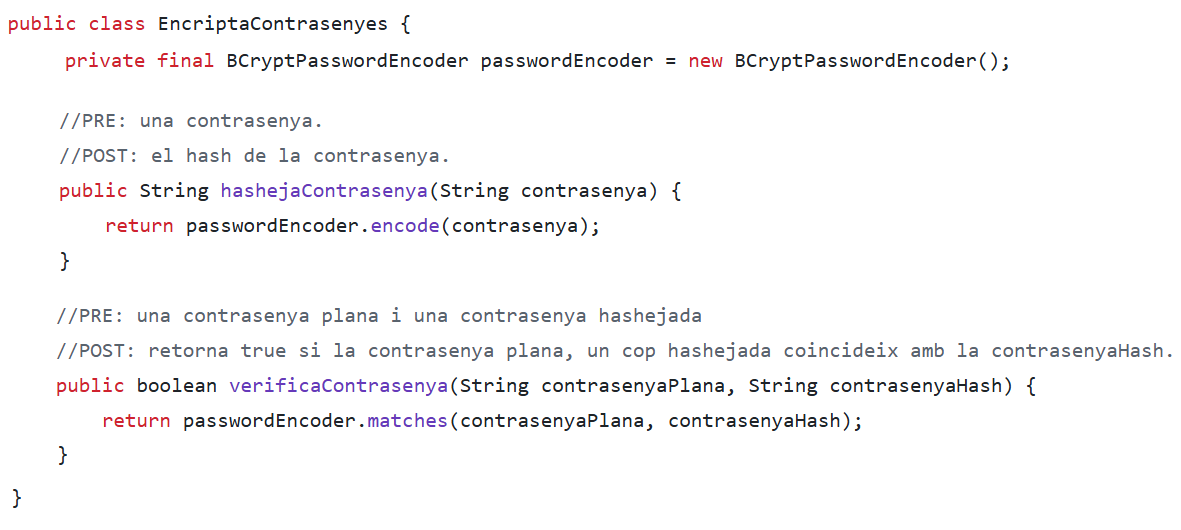
\includegraphics[width=1\linewidth]{img/hashejatContrasenyes.png}
			\end{figure}
			\FloatBarrier
			
			Específicamente, cada vez que un usuario inicie sesión o se registre, se utilizarán una u otra función de la clase \href{https://github.com/blackcub3s/mercApp/blob/main/APP%20WEB/__springboot__produccio__/app/src/main/java/miApp/app/utils/EncriptaContrasenyes.java}{EncriptaContrasenyes.java}. Al instanciar un objeto de la misma, se instanciará también un objeto BCryptPasswordEncoder y se usarán las funciones de librería \textit{encode()}\footnote{Para obtener el hash de una contraseña creada.} y \textit{matches()}\footnote{Para verificar si una contraseña plana es coincidente con el hash que se guardó en base de datos en el momento del registro.}, respectivamente (convenientemente guardadas con un nombre más agradable como vemos en la figura \ref{fig:hashejatContrasenyes}).
			
			Esto se hará en la clase de servicio \textit{UsuariServei.java}. Por ejemplo, para el inicio de sesión el uso de \textit{matches()} a través de \textit{ verificaContrasenya()} lo encontraremos en esta línea de código de dicha clase:  \href{https://github.com/blackcub3s/mercApp/blob/e8afa7110971dca00a660bd8ec5f1a565b852fbd/APP%20WEB/__springboot__produccio__/app/src/main/java/miApp/app/Usuaris/servei/UsuariServei.java#L67}{link}.
			

			
			
			¡Es interesante hacer notar que una misma contraseña encriptada varias veces por la función \textit{encode()} (envuelta en \textit{hashejaContrsenya()}) produce hash distintos! Es decir, el hashing no solo imposibilita ver las contraseñas de los usuarios, sino que también impide ver si dos usuarios tienen la misma contraseña. Esto también hace que no podamos comparar con una función simple de comparación de strings el hash guardado de una contraseña en el momento del registro con el hash generado por un logueo. Por eso nos vemos obligados a usar el metodo \textit{matches()}.
			
			
			
			
			

			
	\section{Desarrollo back-end (microservicio con Python)}
	
	\subsection{Contenerización}
	\label{sec:conteneritzacioPython}
	
	Este microservicio lo contenerizaremos gracias a este \href{https://github.com/blackcub3s/mercApp/tree/main/APP%20WEB/__FastAPI__/Dockerfile}{Dockerfile}. Para hacerlo, usaremos el Dockerfile para crear una imagen desde la imagen python:3-11 alpine\footnote{Las imágenes alpine son ligeras: pesan 100 o 200MB a diferencia de las que provienen de la imagen entera de python, que pesan más de 1GB.} descargada del registry de docker (ver nota sobre instalación de docker\footnote{ Instalar docker en linux no se puede hacer con un solo comando. Si el lector lo quiere instalar y usa linux, le facilito el script que programé hace un tiempo, para poder instalarlo sin preocuparse de nada: \href{https://github.com/blackcub3s/mercApp/blob/main/auxiliars/instalaDocker.sh}{link}. Si el lector usa Windows solamente debe preocuparse de instalar docker desktop y asegurarse que se añade la docker CLI para poder usar comandos desde las terminales disponibles en el sistema.}). 
	
	Para crear la imagen con este Dockerfile, para hacer pruebas y ver como se despliega el contenedor, el lector puede probar de crear una imagen denominada ``back-end-fastapi''. Para hacerlo puede moverse a donde está el Dockerfile y ejecutar el siguiente subcomando de docker (\textit{build}), tal que así:
	
	\begin{lstlisting}[language=bash]
		docker build -t back-end-fastapi .
	\end{lstlisting}
	
		Ahora la imagen ``back-end-fastapi'' ya está creada y con docker images veremos que así es (figura \ref{fig:dockerimages}):
	\FloatBarrier
	\begin{figure}[H]
		\centering
		\caption{comando docker images para ver las imágenes creadas}
		\label{fig:dockerimages}
		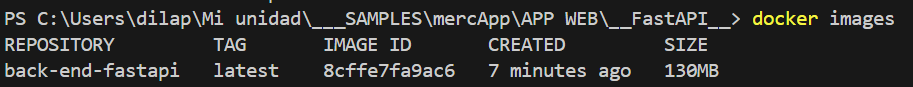
\includegraphics[width=1\linewidth]{img/dockerImages}
	\end{figure}
	\FloatBarrier
	

	
	Acto seguido, una vez ya creada la imagen que contendrá todo el sistema de archivos de la aplicación con Python y sus dependencias (\textit{pip install ...}), debemos usar esta imagen para derivar de ella un contenedor (es decir, crear una instancia de esa imagen). Crearemos el contenedor de nombre \textit{contFastApi} a partir de la imagen anterior y le pediremos que exponga el puerto 8000\footnote{Hacer referencia al 8000 que va a la \textbf{derecha} de los dos puntos.} -puerto con el que se comunica fastAPI en el interior del contenedor- y haremos que exponga ese puerto también al exterior del contenedor\footnote{Es el 8000 emplazado a la \textbf{izquierda} de los dos puntos.}. Podemos hacerlo con run o con create. En este caso con create porque no queremos todavía ejecutarlo:
	
	\begin{lstlisting}[language=bash]
docker create -p 8000:8000 --name contFastApi back-end-fastapi
	\end{lstlisting}

	
	Una vez creado el contenedor ya podemos arrancarlo. Aqui ya no hay que definir puertos nuevamente porque ya se definieron al crear la imagen. Es también opcional usar las flags -a\footnote{Simplemente veremos lo que imprima la terminal} e -i\footnote{Nos permitiría interaccionar con el programa a través de la terminal si fuese necesario}:
	
	\begin{lstlisting}[language=bash]
		docker start -ai contFastApi
	\end{lstlisting}
	
	
	Ahora el contenedor se podría acceder a través de otro contenedor. Nótese que  \href{https://github.com/blackcub3s/mercApp/blob/cf678ebf99ce636b64c70c8faa239658a601550d/APP%20WEB/__FastAPI__/Dockerfile#L22}{en esta línea} del dockerfile hemos definido el host de la aplicacion fastAPI desde dentro del contenedor para que sea la IP 0.0.0.0 . \textbf{No }hemos usado la IP loopback por defecto (localhost, loopback o 127.0.0.1), sino la IP ``wildcard'' o dirección de red (0.0.0.0). Si usáramos la localhost dentro del contenedor la aplicación estaría usando la direccion de dentro de la red del contenedor, pero no saldría fuera de este y sería inútil! La dirección 0.0.0.0 nos permite justamente que podamos acceder a los endpoints de fastAPI desde el localhost del sistema host no solo desde el localhost del propio contenedor. Es decir, no spermite que podamos acceder desde el navegador de nuestro ordenador -fuera del contenedor- o desde otros contenedores corriendo en nuestra máquina. Véase en la figura \ref{fig:demofastapiendpointdummy} siguiente lo que puede hacer nuestro contenedor con esta configuración y como se construye, de forma más pormenorizada:
	
	\FloatBarrier
	\begin{figure}[H]
		\centering
		\caption{definición de un endpoint de fastApi que correrá dentro del contenedor docker contFastApi (subcaptura A)), configuración del comando para correr fastAPI dentro de los contenedores que se instancien a partir de la imagen del Dockerfile, con la dirección de red 0.0.0.0 que permite exponer endpoints de contenedores que se creen con la misma fuera de esos contenedores (B) rectángulo rojo). También podemos ver la configuración de que fastAPI correrá en el puerto 8000 \textbf{dentro} del contenedor instanciado (B) rectángulo verde). Finalmente, podemos ver también el comando que crea finalmente contenedor desde la imagen, pidiéndole que que escuche en el puerto 8000 de la red interna del contenedor (C) rectángulo verde) y lo de ahí lo saque al puerto 8000 (C) rectángulo naranja) siendo el resultado de la exposición del endpoint observable en nuestro equipo anfitrión del contenedor en el localhost en ese mismo puerto 8000 (D), rectángulo naranja).}
		\label{fig:demofastapiendpointdummy}
		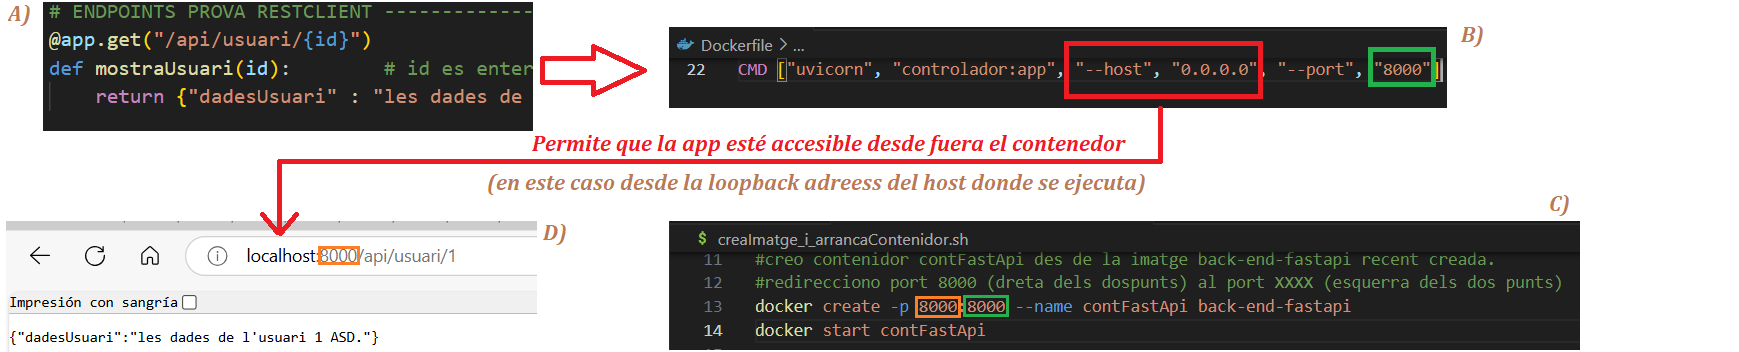
\includegraphics[width=1\linewidth]{img/demoFastApiEndpointDummy}
	\end{figure}
	\FloatBarrier
	
	Para automatizar el proceso de crear imagen con fastAPI y arrancar contenedor desde esta imagen y, finalmente, exponer los endpoints de fastAPI fuera del contenedor, puede usarse el script en bash \href{https://github.com/blackcub3s/mercApp/blob/main/APP%20WEB/__FastAPI__/creaImatge_i_arrancaContenidor.sh}{creaImatge\_i\_arrancaContenidor.sh}, que incluye todos los comandos necesarios (inclusive aquellos para parar y destruir contenedores antiguos) ubicado aqui (ver figura)
	
	\subsection{estructura de la aplicación}
	
	
	\subsection{Algoritmo de extracción}
	
	La extracción de los tikets se hará a partir de la dirección de correo electrónico con la que mercadona manda los tikets digitales (como podemos ver en \ref{sec:pas4googleAPIclient}). El correo electrónico más antiguo y más nuevo prácticamente no difieren, con lo cual se puede reaprovechar un mismo algoritmo para todos los tickets como podemos ver en la imagen \ref{fig:primerIultimTiketMeuCorreu}:
	
	
	
	\FloatBarrier
	\setlength{\belowcaptionskip}{3pt}
	\begin{figure}[H]
		\centering
		\caption{A la \textbf{izquierda}: la primera compra en Mercadona hecha con ticket digital por mi parte: en un supermercado en Catalunya; a la \textbf{derecha} la última compra que se ha hecho por mi parte: en la comunitat valenciana. Nótese que en la extracción hay que tener en cuenta el distinto idioma que se puede dar en distintas comunidades autónomas. La dirección desde la que se mandan los tickets digitales no ha cambiado en dos años y el formato general del tiket es exactamente igual a términos de parseo: Hay que prestar atención a posibles problemas con el unicode (círculo marrón).}
		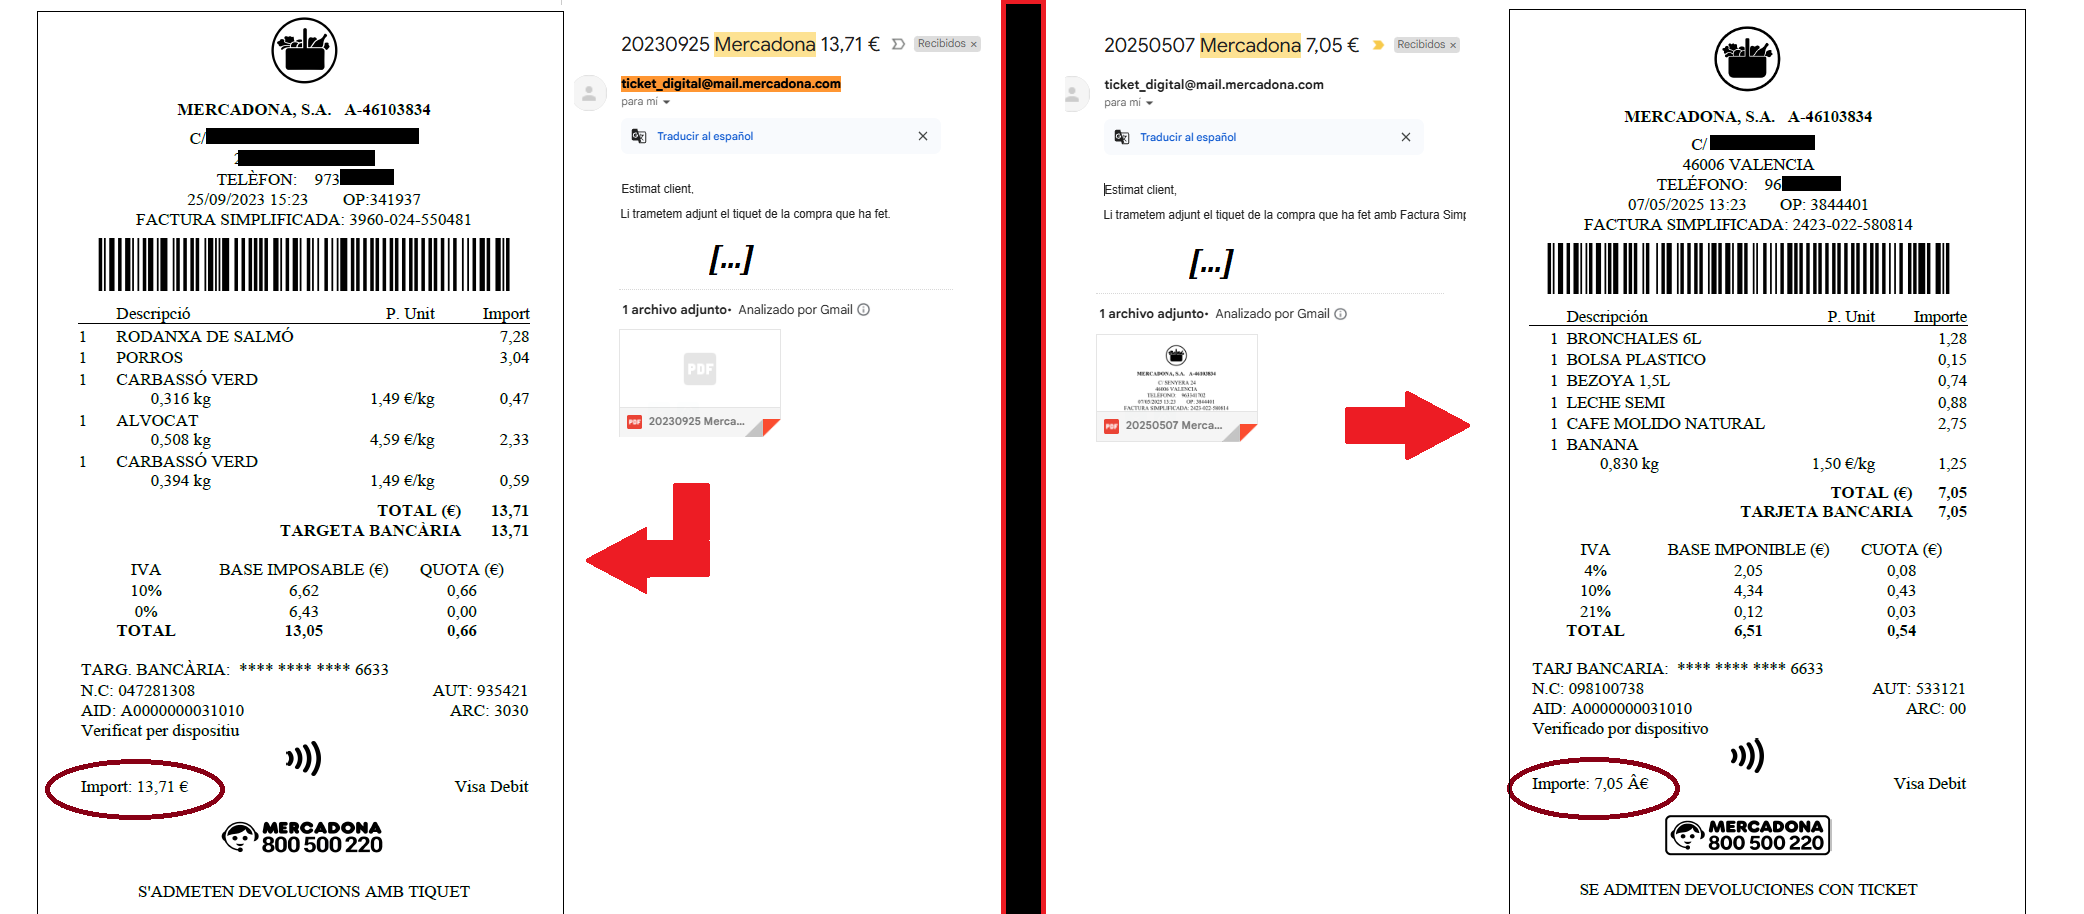
\includegraphics[width=1\linewidth]{img/primerIultimTiketMeuCorreu}
		\label{fig:primerIultimTiketMeuCorreu}
	\end{figure}
	\FloatBarrier
	
	
	
	
	
	\section{Desarrollo del front-end}
	
	\subsection{Contenerización}
	
	Se ha utilizado un servidor de alto rendimiento para servir los archivos estáticos (HTML, CSS y JavaScript). Podéis ver su dockerfile \href{https://github.com/blackcub3s/mercApp/blob/main/APP%20WEB/__frontend__produccio__/Dockerfile}{aquí}, y el script que crea la imagen e instancia de contenedor \href{https://github.com/blackcub3s/mercApp/blob/main/APP%20WEB/__frontend__produccio__/creaImatge_i_arrancaContenidor.sh}{aquí}. Para más información del uso de Docker podéis ver el apartado \ref{sec:conteneritzacioPython} de la contenerización de Python.
	
	\subsection{Estructura de la aplicación}
	\label{sec:estructuraAplicacionFrontEnd}
	
	\textbf{TO DO}
	
	\subsection{Enrutamiento de vistas}
	\label{sec:EnrutamientoDeVistas}
	
	Cuando un usuario introduzca su correo en el formulario de registro de la página principal de la web (\texttt{pas1\_LandingSignUp.html}, que renombraremos a \texttt{index.html}) va a ser redirigido con javascript a partir de las llamadas al back-end de Spring Boot: éste ultimo nos permitirá acceder al valor de la variable ``permisos'' de la tabla ``usuaris'' de mySql, siendo así redirigido a unas páginas u otras (el asunto de como se evita que ciertas páginas sean vistas por usuarios ya autenticados se cubre en otra sección: apartado \ref{sec:vistasPermisos}).
	
	

	
	Estas redirecciones no son fruto del azar. Se ha hecho un proceso de desarrollo inverso del proceso de registro de la plataforma NetFlix: replicándolo, desde cero, y adaptándolo a nuestro caso particular. Si Netflix utiliza ese esquema es porque tiene un impacto en la facilidad de captación de clientes y qué mejor que tratar de replicar los sistemas de los grandes \textit{players}.
	
	\setlength{\belowcaptionskip}{3pt}
	\FloatBarrier
	\begin{figure}[H]
		\centering
		\caption{\textbf{Imagen superior}: Detalle de la landing page \texttt{pas1\_LandingSignUp.html} (\texttt{index.html}) donde el usuario introducirá inicialmente su correo para registrarse -aunque ese mismo formulario en realidad nos servirá para todo gracias al enrutamiento de vistas- $||$ \textbf{Imagen inferior}: la página de Netflix en la que nos hemos inspirado para el diseño minimalista.}
		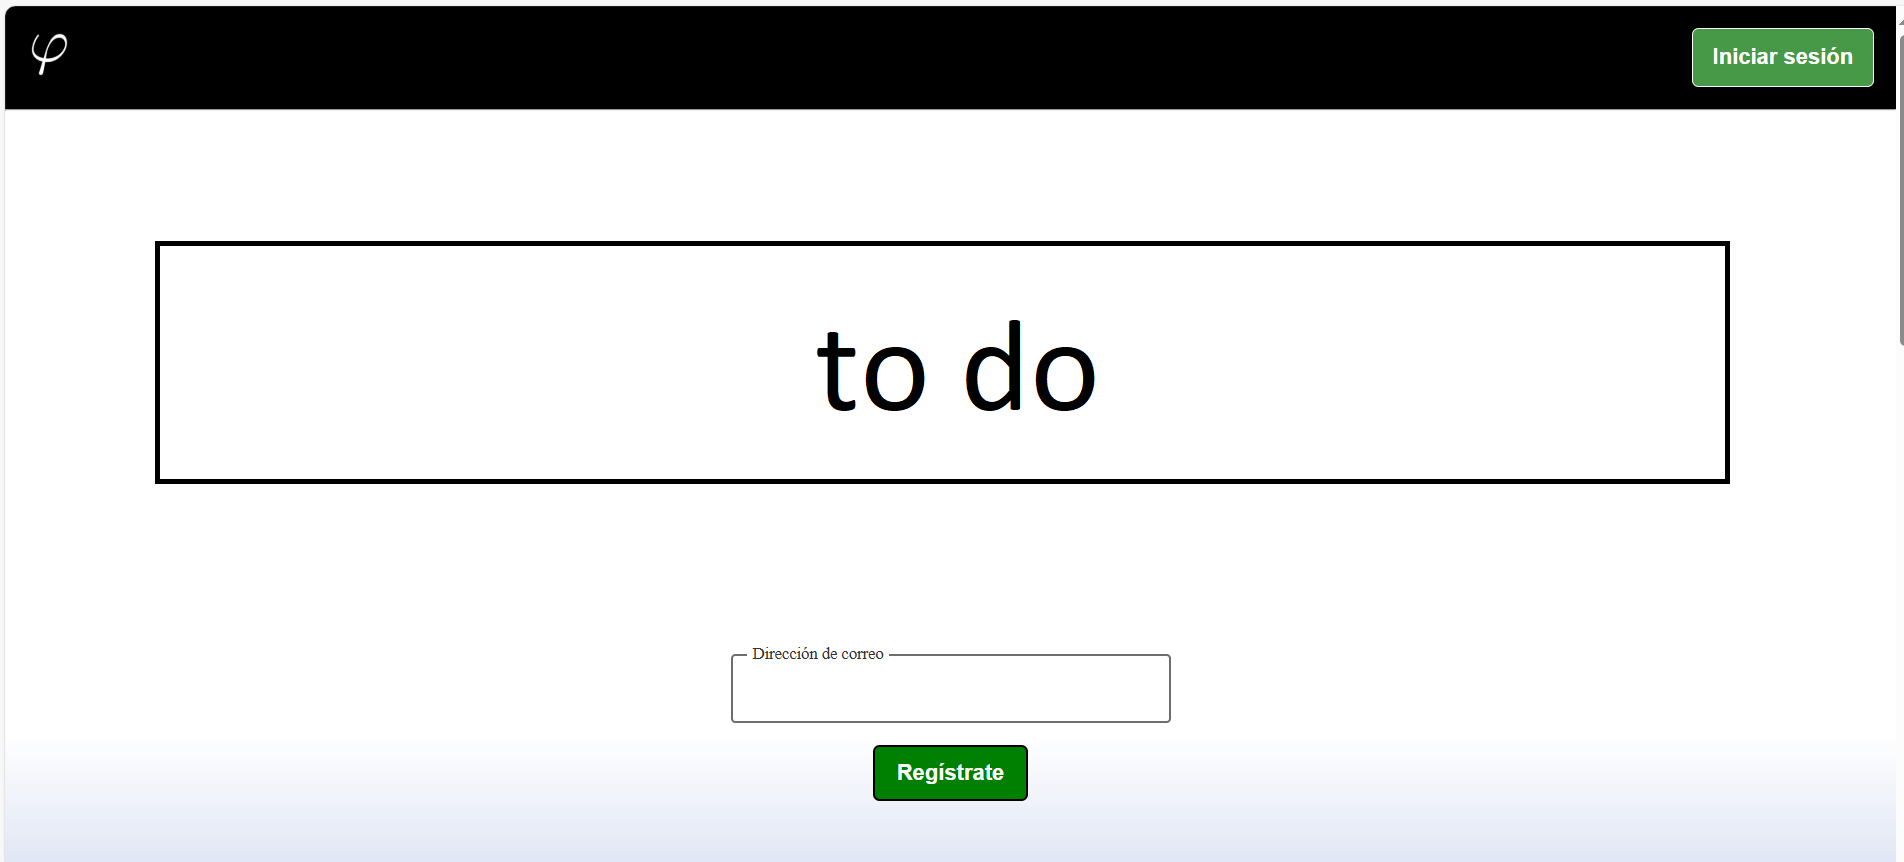
\includegraphics[width=1\textwidth]{img/landingSignUp.png}

		\label{fig:landingSignUpDETALL} 
	\end{figure}
	\FloatBarrier
	
	El esquema simplificado del proceso de enrutamiento durante el registro de un usuario en NetFlix queda recogido en el diagrama del anexo (ver apartado \ref{sec:anexo_diagramaNetflix}) y puede consultarse también en uno de los repositorios de mi github (\href{https://www.github.com/miApp}{link}). 
	
	Asimismo, el proceso de registro que utilizamos en mercApp es convenientemente una derivación de este mismo: si bien en NetFlix primeramente se redirige al usuario a unas cartas de pago, nosotros aquí le llevamos a una página para que nos dé acceso al gmail en el que Mercadona los tickets digitales al usuario (la página  \texttt{pas4\_ConcedirAccesGmail.html}); de nuevo análogamente a NetFlix, donde al usuario que ya ha pagado se le concede inmediatamente el acceso a las películas y series,  en nuestro caso se le dará acceso al usuario al tablón de visualización de análisis de datos de los tikets digitales  (\texttt{dashboard.html}), donde se visualizan el resultado de la minería y extracción de datos de esos tikets. 
	
	El proceso de enrutamiento de los usuarios desde que introducen el correo en el formulario de \texttt{pas1\_LandingSignUp.html} (\texttt{index.html}) hasta que acceden al \textit{dashboard} se encuentra recogido en el diagrama de la figura \ref{fig:diagramaMercaAppFront}, cuyas nomenclaturas explicamos en los siguientes \textit{bullet points}:
	\vspace{1em}
	\hrule
	
	\begin{itemize}
		\setlength{\itemsep}{-.3em}
		
		\item Decisiones del back-end de Spring Boot al llamar a APIs: \textbf{\textcolor{yellow!75!black}{\underline{rombos amarillos}}}. %75 per cent groc i 25 negre entenc
		\item Las APIs que consume el front-end van entre corchetes ([]) y con color:
		\begin{itemize}
			\setlength{\itemsep}{.0em}
			\item \textbf{\textcolor{red}{[\texttt{/api/avaluaUsuari}]}}: \textit{end-point} que evalúa si el correo electrónico introducido pertenece a un usuario registrado y qué permisos tiene.
			\item \textbf{\textcolor{brown}{[\texttt{/api/registraUsuari}]}}: \textit{end-point} que registra un nuevo usuario en el sistema y expide su AccessToken con permisos a 0 en las \textit{claims} de su \textit{payload}\footnote{El lector puede consultar la explicación sobre lo que son las claims y el payload de un JWT en el apartado \ref{sec:queComponeJWTbackend}.}.
			\item \textbf{\textcolor{blue}{[\texttt{/api/login}]}}: \textit{end-point} que gestiona el proceso de autenticación y generación del \textit{JWT Access Token} con tres niveles de permisos posibles (0, 1 y 2).
		\end{itemize}
		
		
		
		\item Las vistas -archivos html- a las que redirige JavaScript mediante la llamada a $window.location.href$ a partir de los resultados de las llamadas a las APIs:  \textbf{\textcolor{orange}{\underline{rectángulos naranja}}}.
		
		\item Expedición de tokens de acceso (JWT) desde el endpoint del que emanan y enviados al front-end se representan con un rectángulo \textbf{\textcolor{blue!40!white}{\underline{de fondo azul}}} y bordes redondeados \footnote{Consultad la estructura de los mismos en la figura \ref{fig:jwtioMostraPayload}.}.
		
	\end{itemize}
	
	
	
	
	\setlength{\belowcaptionskip}{3pt}
	\FloatBarrier
	\begin{figure}[H]
		\centering
		\caption{Diagrama de flujo del enrutamiento completo del sistema \textit{front-end} durante el proceso de registro, desde que el usuario introduce su correo en \texttt{pas1\_LandingSignUp.html} (\texttt{index.html}) hasta obtener acceso al \texttt{dashboard}.\\ -------------------- \textit{NOTA:} \textbf{Acceso a recursos $\iff$ permisos $\geq$ 1} --------------------}
		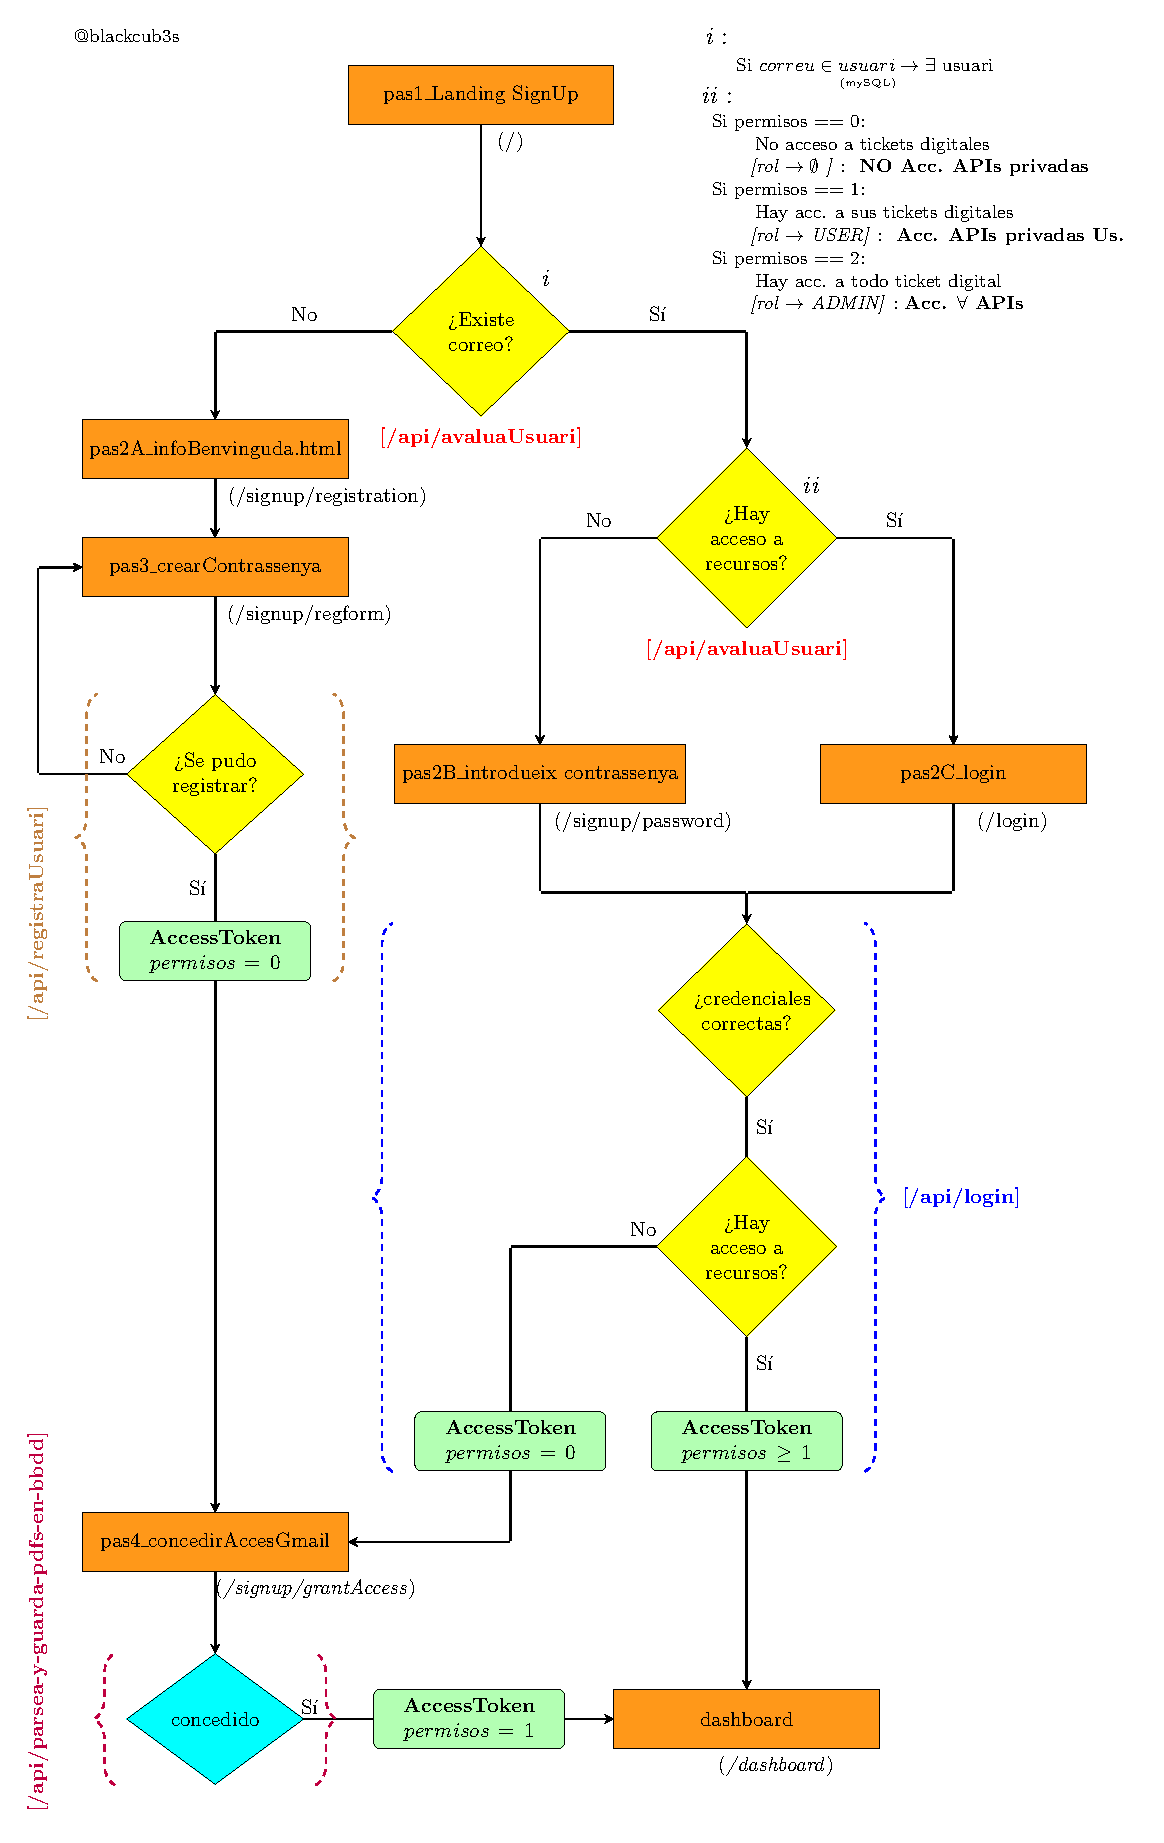
\includegraphics[width=1\textwidth]{img/diagramaMercAppFront.pdf}
		
		\label{fig:diagramaMercaAppFront} 
	\end{figure}
	\FloatBarrier
	
	
	
	
	
	
	
	
	\subsection{Manejar vistas en función de Autenticación y autorización}
	
	
	Como hemos visto antes Podemos considerar que cada archivo HTML y su CSS asociado es una ``vista'' de nuestra aplicación. Habrá vistas que \textbf{no nos interesará enseñar a ciertos usuarios}, porque o bien no serán relevantes para ellos o bien harán llamadas a APIs cuya información no podrá ser obtenida para ellos.
	
	Si bien Spring Boot permite servir los archivos estáticos\footnote{HTML, CSS y JS son archivos estáticos.}  de dentro del mismo back-end de Spring Boot y utilizar un sistema de plantillas (Thymeleaf) que permite impedir visualizaciones de vistas a usuarios no autorizados, esto realmente no es, para nada, lo ideal. Lo ideal es definir un front-end y un back-end separados partiendo de principios de \textit{separación de responsabilidades} o \textit{SoC}\footnote{Separation of concerns}, y así lo hemos hecho en este proyecto\footnote{Si tenemos ambas partes desacopladas podremos hacer modificaciones independientes en ambas. Por ejemplo, podremos cargar los archivos front-end en una CDN o un Proxy o tenerlos cacheados en un servidor que los sirva mucho más rápido, como Nginx. Es más, lo óptimo sería generar los archivos del front-end mediante un sistema de desarrollo por componentes (como Angular, React o Vue) para facilitar el desarrollo cuando la aplicación crezca y utilizar una paradigma \textit{SPA} (\textit{Single Page Application}). Sin embargo, en este caso, por el tiempo disponible y el tamaño de la aplicación se ha optado por hacerlo con HTML, CSS y JS puros.}. Las ventajas son grandes y tienen implicaciones en términos de mantenimiento, escalabilidad y reutilización tanto del front-end como del back-end (ver ventajas justificadas en anexo \ref{sec:SoCVENTATJES}).
	

	
	
	
	
	Sin embargo, no todo es ideal. Siempre existen concesiones (o como diríamos en inglés ``trade-offs''). Al tener el front-end y el back-end desacoplados esto también aumenta considerablemente la complejidad inicial en el desarrollo: la protección de las vistas a usuarios que no deben visualizarlas se hace más difícil porque no las sirve el back-end y no las puede proteger directamente este\footnote{A diferencia de lo que sí haría una aplicación back-end hecha en php tradicional como las que hemos visto en desarrollo web entorno servidor, donde servimos el HTML desde dentro del mismo PHP).}.
	
	Por ejemplo, del mismo modo que los endpoints de nuestra API del back-end en Spring Boot están protegidos y no devuelven datos cuando el JWT de acceso que tengamos en el front-end haya caducado, sea inexistente, o sea inválido (porque haya sido manipulado o no tenga en el \textit{payload} el ``idUsuari'' que permita el acceso a un cierto recurso), también pasará que ciertas páginas del front-end no podrán obtener la información deseada si llaman a un end-point para el que no tienen autorización: en este caso ello tendrá implicaciones para las vistas, y deberemos modificar su DOM para la ocasión mostrando un mensaje de error, instando al usuario a iniciar sesión y/o bien redirigir al usuario a la página correcta, por ejemplo. Nosotros hemos optado por este último enfoque.
	
	Con tal de conseguirlo, deberemos manejar la lógica en cada caso particular desde el front-end usando JavaScript. Tengo entendido que en frameworks como Angular esto se puede hacer de forma muy sencilla, solo definiéndolo en una ocasión. Aquí cada página particular requerirá una programación específica con JavaScript para redirigir a los usuarios.
	
	\subsubsection{Protegiendo vistas ``privadas'' ante usuarios no ``logueados'': cuando el token ha expirado}
	
	Existen dos páginas de nuestra web que, cuando expire el token de acceso que se requiere para acceder a los recursos back-end que hay detrás de ellas (o este no exista), no deberán ser visualizables:
	
	\vspace{0em}
	\begin{itemize}
		\setlength{\itemsep}{-.5em}
		\item \texttt{pas4\_concedirAccesGmail.html}
		\item \texttt{dashboard.html}
	\end{itemize}
	
	Como se desprende del diagrama de flujo del enrutamiento del proceso de registro que vimos en la figura \ref{fig:diagramaMercaAppFront}, esas dos páginas son aquellas páginas de nuestro proyecto a las que redirigimos los usuarios justo después de generar tokens de acceso; por ende, su visionado requiere cierto grado de autenticación y autorización. De ahí que consideremos no permitir visualizarlas si el grado de permisos requerido no se llegase a satisfacer.
	
	La primera página (\texttt{dashboard.html}), requiere tener un token con permisos a 0; la segunda (\texttt{pas4\_concedirAccesGmail.html}) un token con permisos superior o igual a 1. En otras palabras: ambas requieren tener algún tipo de autenticación de usuario que se materialice en un token de acceso con una variable de permisos (i.e a esto nos referimos con usuarios ``logueados'' en el título), como veremos en el siguiente apartado; pero está claro que para visualizar cualquiera de estas dos páginas o vistas, la condición \textit{sine qua non} comuna es que dentro de \textit{localStorage.getItem(``AccessToken''}) se albergue un token de acceso que \underline{no esté expirado} y que sea \underline{descifrable}\footnote{Ojo, descrifrable no significa validable. Validable es lo que hacemos en el back-end con el secret, y no se muestra jamás en el cliente.}.
	
	Si está expirado, cuando hagamos la diferencia entre el valor ``exp'' del payload\footnote{Segundos en que el token expira o expiró, desde la epoch.} y la función \textit{Date.now()/1000}\footnote{Segundos actuales del navegador, desde la epoch.} saldrá un número negativo. En caso contrario, positivo. 
	
	Si el token está expirado -o es inexistente- inmediatamente redirigiremos al usuario a la landing page llamando a \textit{redirigeixAlandingPage()}, impidiendo así el visionado de cualquiera de las dos páginas (se cargará el script que contiene esta función antes de que se cargue el DOM\footnote{El lector puede hacer la prueba siguiente: si el token ha caducado o el usuario no se ha logueado, accediendo a \texttt{pas4\_concedirAccesGmail.htm} o a \texttt{dashboard.html} verá como automáticamente se produce una redirección a \texttt{pas1\_landingSignUp.html} (\texttt{index.html}); o si se ha logueado, abrir la consola y verá una cuenta atrás del tiempo que le queda al token de acceso para su expiración y para la redirección a la landing page.}). En cambio, si el token no está expirado seguiremos revaluando la expiración del token -y su existencia- con una frecuencia de un segundo: esto se conseguirá mediante la función asíncrona \textit{setInterval()} que hemos visto en desarrollo web entorno cliente de segundo curso.
	
	Para ello, en el \textit{head} de cada una de las dos páginas en cuestión veréis que \textbf{antes} siquiera \textbf{de cargar el DOM} se cargan sendos archivos:
	
\begin{lstlisting}[language=xml, basicstyle=\ttfamily\footnotesize, keywordstyle=\color{magenta}]
<script src="/js/jwt/decodificaJWT.js"></script>
<script src="/js/jwt/restringeixVistesPrivades_USUARI_NO_LOGUEJAT.js">
</script>
\end{lstlisting}
	
	En el primero tenemos la función para extraer el payload de un token. Y en el segundo está la lógica que acabamos de explicar en los párrafos anteriores (ver figura \ref{fig:restringeixVistesPrivades_USUARI_NO_LOGUEJAT}):
	
	
	\setlength{\belowcaptionskip}{3pt}
	\FloatBarrier
	\begin{figure}[H]
		\centering
		\caption{Script \texttt{restringeixVistesPrivades\_USUARI\_NO\_LOGUEJAT.js}, utilizado para regresar automáticamente a la landing page cuando el token de acceso de un usuario logueado expira -o es borrado- o cuando un usuario no logueado intenta acceder a las páginas que requieren permisos de acceso: \texttt{pas4\_concedirAccesGmail.html} y \texttt{dashboard.html}.}
		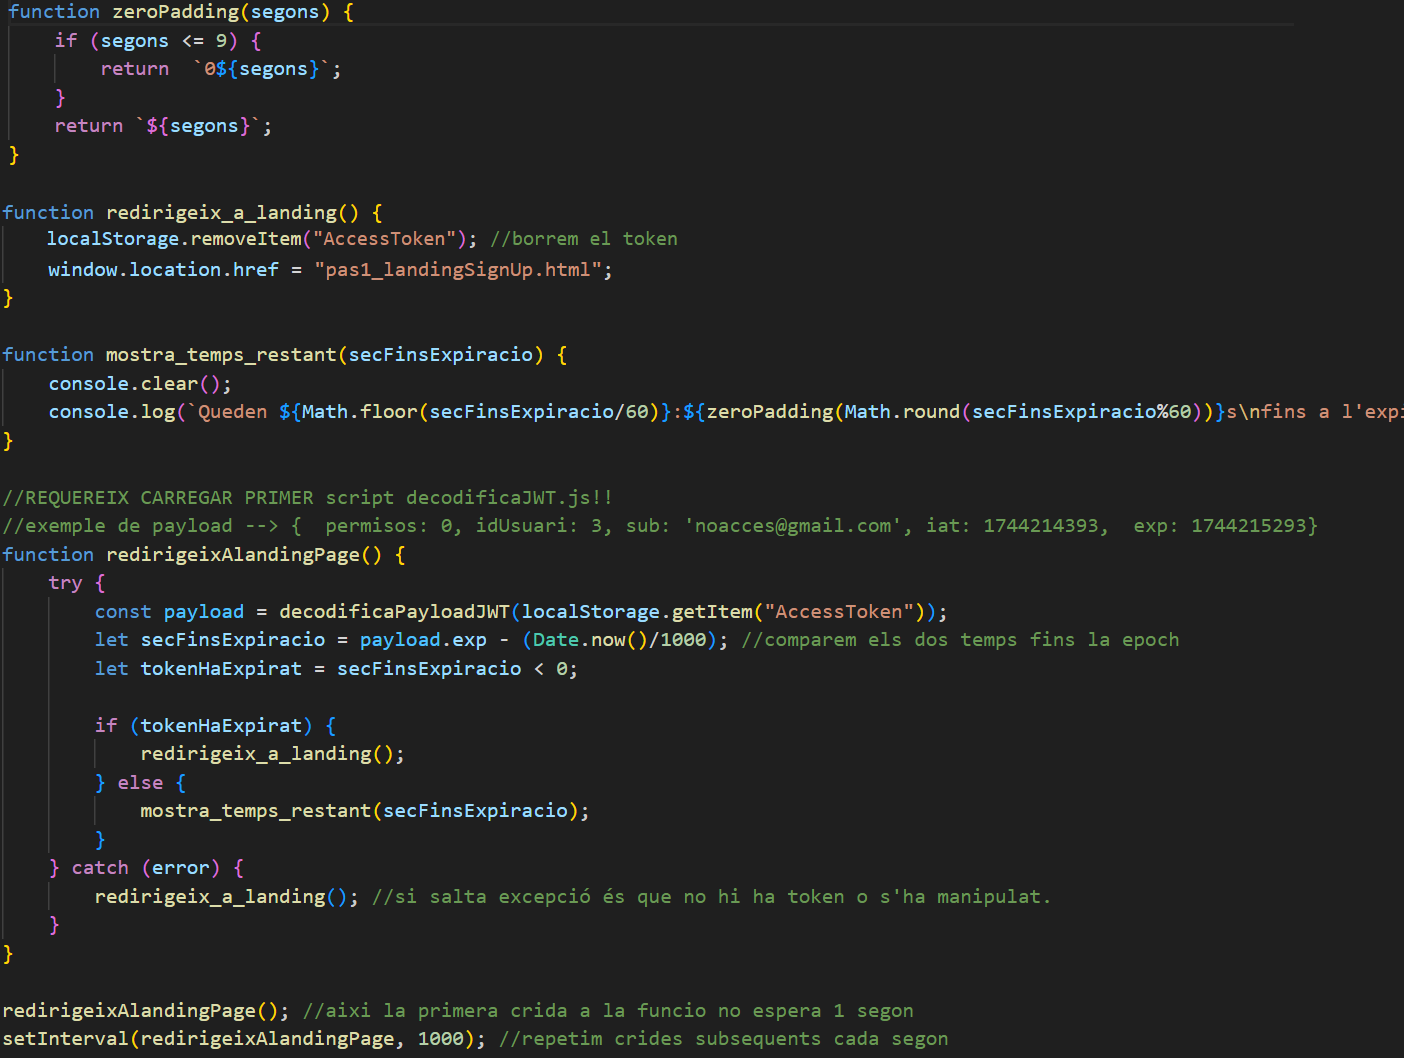
\includegraphics[width=1\linewidth]{img/restringeixVistesPrivades_USUARI_NO_LOGUEJAT.png}

		\label{fig:restringeixVistesPrivades_USUARI_NO_LOGUEJAT}
	\end{figure}
	\FloatBarrier
	
	\subsubsection{Protegiendo vistas ``públicas'' para usuarios ``logueados'': cuando el token no ha expirado}
	\label{sec:vistasPermisos}
	

	
	Para empezar, es necesario mencionar que se establecen tres niveles de permisos en la aplicación: estos  tienen un impacto sobre qué puede visualizar el usuario ``logueado'' y qué no; y cómo se permite que el usuario navegue a medida que va moviéndose en el proceso de registro cuando no está ``logueado''.
	
	Antes ya hemos visto que estos permisos nos han permitido construir el enrutamiento del front-end de la aplicación (su impacto podemos verlo en la parte superior derecha de la figura del enrutamiento \ref{fig:diagramaMercaAppFront} y más resumidamente en el cuadro \ref{table:permisos}), pero también ahora debemos utilizarlos también para \textbf{impedir} visualizar ciertas páginas en usuarios \underline{ya logueados}, es decir, aquellas páginas a las que nos referimos con el término ``vistas públicas'' empleado en el título de esta sección.
	
	\begin{table}[H]
		\centering
		\caption{Significado de la variable \texttt{permisos} en la tabla \texttt{usuaris} de mySQL.}
		\begin{tabular}{|c|l|}
			\hline
			\textbf{\texttt{permisos}} & \textbf{Significado} \\
			\hline
			0 & No hay acceso a tickets digitales (pero ya tenemos email y contraseña) \\
			1 & Acceso a tickets como usuario (USER) \\
			2 & Acceso a tickets como administrador (ADMIN) \\
			\hline
		\end{tabular}
		\label{table:permisos}
		
	\end{table}
	
	Programáticamente, debemos conseguir que estas ``vistas públicas'' \textbf{no sean visualizables} jamás si, en el \textit{local storage}, \textbf{existe}  un \underline{token de acceso} que \textbf{no haya expirado}\footnote{¡Si existe ese token no expirado significa que el usuario ya no debe acceder a ellas, porque ya se ha registrado y/o iniciado sesión y solo debe ver páginas de usuario registrado!}. Estas páginas vetadas a los usuarios ``logueados'' son las siguientes:
	
	\vspace{0em}
	\begin{itemize}
		\setlength{\itemsep}{-.5em}
		\item \textit{A)} \texttt{pas1\_landingSignUp.html} (\texttt{index.html})
		\item \textit{B)} \texttt{pas2A\_infoBenvinguda.html}
		\item \textit{C)} \texttt{pas2B\_introduirContrasenya.html}
		\item \textit{D)} \texttt{pas2C\_login.html}
		\item \textit{E)} \texttt{pas3\_crearContrasenya.html}
	\end{itemize}
	
	La forma que optamos para impedir su visualización es poner \textbf{dos scripts} en cada una de las cinco vistas públicas arriba mencionadas, que permitirán redirigir al usuario a la página ``privada'' que le corresponda según el valor que toma la variable ``permisos''\footnote{No hace falta mencionar que se saca del campo permisos de la tabla usuaris de la base de datos que tenemos en mySQL.} dentro del \textit{payload} del token de acceso guardado en el \textit{local storage} \footnote{Si queréis ver a qué me refiero con el payload, revisad de nuevo la figura \ref{fig:jwtioMostraPayload}.}, según se muestra en la tabla siguiente:
		
	\begin{table}[h!]
		\centering
		\begin{tabular}{|c|c|c|}
			\hline
			\textbf{página accedida} & \textbf{Permisos token} & \textbf{Redirigimos automáticamente a} \\
			\hline
			\multirow{2}{*}{\textit{A)}, \textit{B}, \textit{C)}, \textit{D)} o \textit{E)}} & $0$ & \texttt{pas4\_concedirAccesGmail.html} \\
			& $1 || 2$ & \texttt{dashboard.html} \\
			\hline
		\end{tabular}
	\end{table}

	En cada una de las páginas accedidas A), B), C), D) y E), antes que cargue el DOM, los dos scripts mencionados a cargar son:
	
\begin{lstlisting}[language=xml, basicstyle=\ttfamily\footnotesize, keywordstyle=\color{magenta}]
<script src="/js/jwt/decodificaJWT.js"></script>
<script src="/js/jwt/restringeixVistesPubliques_USUARI_LOGUEJAT.js"></script>
\end{lstlisting}

El segundo script, \texttt{restringeixVistesPubliques\_USUARI\_loguejat.js} es una modificación para la ocasión del script mostrado en la figura \ref{fig:restringeixVistesPrivades_USUARI_NO_LOGUEJAT} previa, y lo mostramos a continuación en la figura \ref{fig:restringeixVistesPubliquesUSUARILOGUEJAT}:


\setlength{\abovecaptionskip}{15pt}
\FloatBarrier
\begin{figure}[H]
	\centering
	\caption{Script \texttt{restringeixVistesPubliques\_USUARI\_LOGUEJAT.js}, utilizado para redirigir a un usuario logueado fuera de las páginas públicas de forma automática y directo a las 2 páginas posibles que requieren credencial de acceso (``privadas''), según proceda de acuerdo con la variable permisos de su token de acceso -si el token existe y no ha expirado-: \texttt{pas4\_concedirAccesGmail.html} y \texttt{dashboard.html}.}
	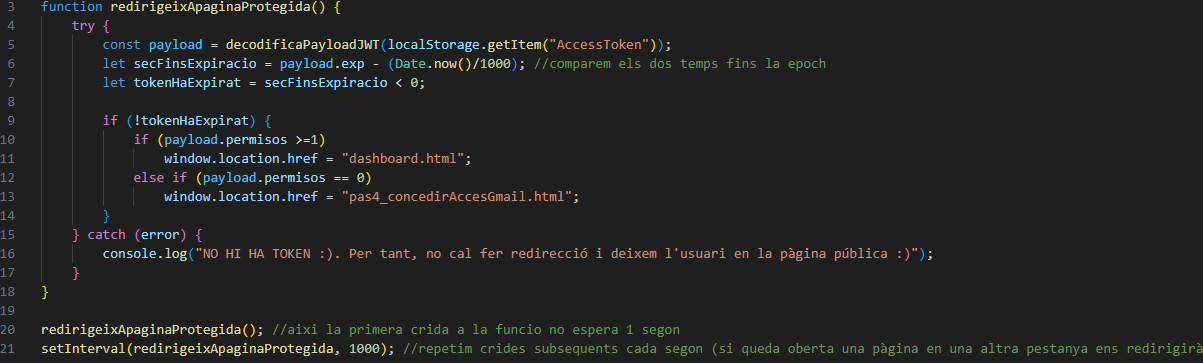
\includegraphics[width=1\linewidth]{img/restringeixVistesPubliques_USUARI_LOGUEJAT.png}
	
	\label{fig:restringeixVistesPubliquesUSUARILOGUEJAT}
\end{figure}
\FloatBarrier	
	


	
\subsubsection{Protegiendo vistas ``privadas'' ante usuarios ``logueados'': cuando el token no ha expirado.}
\label{sec:vistasPermisos}

Análogamente al apartado anterior, tenemos que tomar en consideración las páginas que requieren permisos de acceso. Estas páginas \textit{ya están} protegidas del visionado de usuarios no logueados (usarios que no tengan token expedido): estos no las podrán ver nunca, porque hicimos el script de la figura \ref{fig:restringeixVistesPrivades_USUARI_NO_LOGUEJAT} para redirigilos a la landing page en caso que por error accedan a ellas.

Sin embargo, nos queda algo por hacer: hay que conseguir \textbf{evitar} que un usuario con permisos 1 o 2 en el payload de su token (es decir, que ya ha concedido acceso a tickets digitales) pueda pedir de nuevo acceso a esos tikets; algo completamente innecesario porque ya los ha facilitado a mercApp previamente en \texttt{pas4\_concedirAccesGmail}; o, su opuesto: tenemos que evitar que un usuario con permisos 0 (e.g., ha puesto correo y contraseña y se ha registrado, pero no ha dado acceso a tickets digitales todavía) pueda tratar de visualizar el \texttt{dashboard} a la espera de obtener una información de unos tickets que él todavía no ha proporcionado.

La solución a lo anterior es hacer que en función de los permisos existentes en el token inhabilitemos una vista de las ``privadas'' para el usuario, \textit{mediante} la redirección automática del usuario a la página que sí debe visualizar \textit{antes} de que cargue el DOM de la pagina vetada, tal que así:
	
	\FloatBarrier
	\begin{table}[h!]
		\centering
		\begin{tabular}{|c|c|c|}
			\hline
			\textbf{p. privada accedida
				 (vetada)} &\textbf{Permisos} & \textbf{Redirección automática a} \\
			\hline
			\texttt{dashboard.html} & $0$ &  \texttt{pas4\_concedirAccesGmail.html}\\
			\texttt{pas4\_concedirAccesGmail.html} &$1 || 2$ & \texttt{dashboard.html} \\
			\hline
		\end{tabular}
	\end{table}
	\FloatBarrier

	
	Es decir, en la tabla anterior mostramos que si un usuario con permiso 0 (no ha concedido acceso a tickets digitales) quiere acceder a la página \texttt{dashboard.html} para visualizar la explotación de datos de los tickets, no podrá verla porque le redirigiremos automáticamente a la página donde podrá proporcionar acceso a tickets digitales: \texttt{pas4\_concedirAccesGmail.html}. Y viceversa: Si entra en \textit{pas4} teniendo permisos 1 o 2, será redirigido al \textit{dashboard}. 
	
	Lo que acabamos de mencionar en la última tabla y en el párrafo anterior lo programamos en el siguiente script (cuyo prerequisito será decodificaJWT como en las anteriores ocasiones) y que podemos ver en la imagen \ref{fig:restringeixVistesPrivadesUSUARINOLOGUEJAT}:
	
	
\begin{lstlisting}[language=xml, basicstyle=\ttfamily\footnotesize, keywordstyle=\color{magenta}]
<script src="/js/jwt/decodificaJWT.js"></script>
<script src="/js/jwt/restringeixVistesPrivades_USUARI_NO_LOGUEJAT.js">
</script>
\end{lstlisting} 
	
	
	\setlength{\abovecaptionskip}{15pt}
	\FloatBarrier
	\begin{figure}[H]
		\centering
		\caption{Script \texttt{restringeixVistesPrivades\_USUARI\_LOGUEJAT.js}, utilizado para redirigir a un usuario logueado hacia \texttt{pas4\_concedirAccesGmail.html} o \texttt{dashboard.html}, según proceda, en caso que el usuario entre en una de estas dos páginas privadas sin el permiso correspondiente.}
		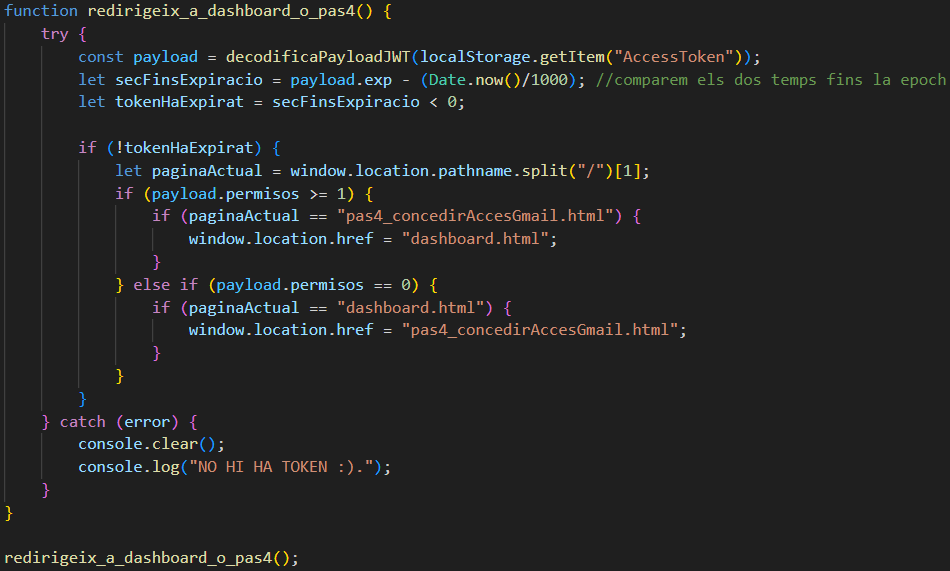
\includegraphics[width=1\linewidth]{img/restringeixVistesPrivadesUSUARINOLOGUEJAT.png}
		
		\label{fig:restringeixVistesPrivadesUSUARINOLOGUEJAT}
	\end{figure}
	\FloatBarrier	
	
	
	
	Para entender como guardamos los datos de permisos e ids de usuario en el front-end, podemos ver el apartado \ref{sec:recibirAccesTokenENFRONTEND} que viene a continuación, donde especificamos como se recibe el token del back-end y se guarda en el front-end.
	
	\subsubsection{Salir voluntariamente de las páginas privadas: botón ``cerrar sesión''}
	\label{sec:tancarSessioBotoExplicacio}
	
	El botón de ``cerrar sesión'' dentro de las dos páginas privadas \texttt{dashboard.html} y \texttt{pas4\_concedirAccesGmail.html} en realidad no cierra ninguna sesión. Recordemos que usamos token de acceso, que sustitye las sesiones. En el botón, sin embargo, hemos decidido mantener el nombre, porque el cierre de sesión es un concepto arraigado en los usuarios de sitios web, incluso más que el concepto de ``salir''\footnote{A nivel de usabilidad se me hace difícil justificar que un usuario diese click a un botón denominado ``eliminar token'' solamente porque el desarrollador quería ser preciso; dejemos esto como una prueba de como en ocasiones la usabilidad viene de la sencillez, no del honor a la verdad.}. 
	
	Lo que hace es , simplemente, eliminar el token de acceso del \textit{localStorage} cuando el usuario clica el botón de id ``botoEliminarToken''. 
	
	En cada una de estas páginas privadas recordemos que tenemos un script que cada segundo está reevaluando si hay token de acceso y si este es válido (ver script de figura \ref{fig:restringeixVistesPrivades_USUARI_NO_LOGUEJAT}). Por lo tanto, si lo borramos ese script va a redirigirnos a la página de inicio como máximo un segundo más tarde de la pulsación del botón de ``cierre de sesión''.
	
	\FloatBarrier
	\setlength{\abovecaptionskip}{15pt}
	\begin{figure}[H]
		\centering
		\caption{Script \texttt{tancaSessioEliminantToken} que elimina el token de acceso cuando el usuario clica en el botón ``cerrar sesión'' en las páginas privadas \texttt{dashboard.html} y \texttt{pas4\_concedirAccesGmail.html}}
		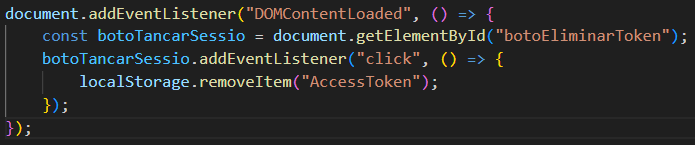
\includegraphics[width=1\linewidth]{img/scriptTancarSessio.png}
		\label{fig:scriptTancarSessio}
	\end{figure}
	\FloatBarrier
	
	
	
	\subsection{Recibir el Access Token desde el back-end}
	\label{sec:recibirAccesTokenENFRONTEND}
	
	Cuando un usuario del que ya tenemos su correo electrónico en BBDD intenta ``loguearse'' en mercApp\footnote{Sea que ya estuvo registrado -permisos 0-, dio acceso a sus tickets digitales -permisos 1- o es superusuario -permisos 2-.}, el token de acceso lo recibe por primera vez en el cliente cuando este haga una llamada fetch() hacia el endpoint del back-end ``\textit{/api/login}''. Esta llamada se hace desde \texttt{pas2C\_login.html} o desde \texttt{pas2B\_introdueix contrassenya.html}, de idéntica forma.
	
	
	Por ejemplo, explicaremos solamente el caso de \textit{pas2Clogin.html}. En este archivo la recepción del token se hará en el JavaScript embedido cuando, por un lado, obtengamos el código 200 (OK) del servidor; pero también, cuando se cumpla que el usuario y contraseña introducidos por el usuario son correctos. Si y solo si se cumplen ambas condiciones, el cliente entonces recibirá el token de acceso en el body de la respuesta a su solicitud, que será una como la que sigue, de la que podremos extraer el ``AccessToken'' y guardarlo inmediatamente en el LocalStorage del navegador: \footnote{Esto lo hacemos para luego poder mandarlo de vuelta al servidor en la subsecuentes solicitudes que requieran autenticación y autorización.} Para más información sobre el código JavaScript del front-end que lo permite véase figuras y \ref{fig:FetchCodisResponseFRONT} y \ref{fig:figuraLoginFetch}):
	
\begin{lstlisting}[language=Java, basicstyle=\ttfamily\footnotesize, keywordstyle=\color{magenta}]
	{
		"usuari": {
			"alies": "the protein kingdom",
			"permisos": 2,
			"idUsuari": 1
		},
		"existeixUsuari": true,
		"AccessToken": "eyJhbGciOiJIUzI1NiJ9.eyJwZXJ [...]",
		"teAccesArecursos": true,
		"contrasenyaCorrecta": true
	}
\end{lstlisting}
	

	
	\setlength{\belowcaptionskip}{3pt}
	\FloatBarrier
	\begin{figure}[H]
		\centering
		\caption{Fragmento de codigo en \texttt{pas2C\_login.html} dentro del codigo javascript para manejar codigos de error. Cuando el back-end de Spring Boot devuelve el código 200 significará que podremos extraer los datos del body de la respuesta. 400 se devolvería si hubiera problemas validación de campos en el back-end,  algo que no debería producirse nunca con el front-end que se ha programado.}
		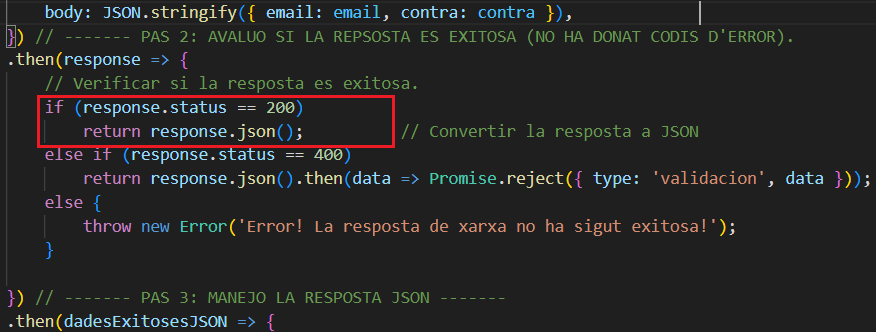
\includegraphics[width=1\textwidth]{img/FetchCodisResponseFRONT.png}
		
		\label{fig:FetchCodisResponseFRONT} 
	\end{figure}
	\FloatBarrier
	
	\setlength{\belowcaptionskip}{3pt}
	\FloatBarrier
	\begin{figure}[H]
		\centering
		\caption{Fragmento de codigo en pas2C\_login.html dentro del codigo javascript para obtener el token de acceso (detalle en rojo).}
		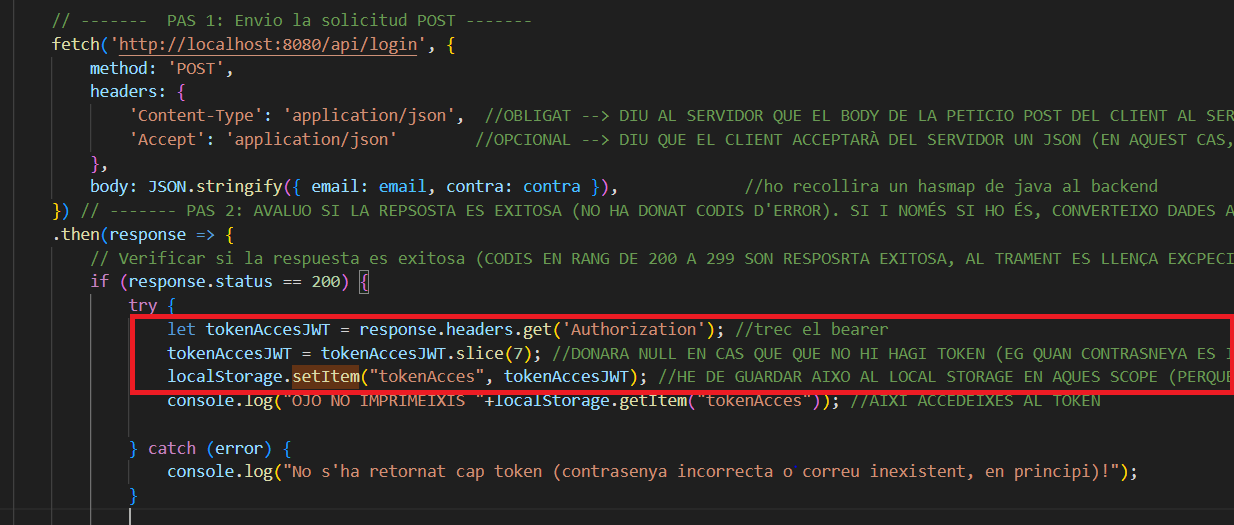
\includegraphics[width=1\textwidth]{img/jwtFetchLoginFront.png}
		
		\label{fig:figuraLoginFetch} 
	\end{figure}
	\FloatBarrier
	
	
	
	Ahora bien, si el usuario nunca se ha registrado en nuestra aplicación\footnote{Es decir, no tenemos su correo electrónico en BBDD.}, cuando lo haga, lo hará por el proceso de registro y no por el proceso de inicio de sesión. Una vez introduzca su contraseña en \texttt{pas3\_crearContrasenya.html} y se tome el correo electrónico insertado por el usuario en páginas previas y guardado en el localStorage, se hará una llamada POST con fetch() al endpoint ``api/registraUsuari'' pasando esos datos por el body: si y solo si el usuario NO existía, se creará un nuevo registro en la tabla Usuaris y ahi se devolverá un JSON con el token de acceso para el nuevo usuario creado, ahora de permisos 0. Este JSON tendrá el siguiente aspecto (el token será mucho más largo):
	
	
	
\begin{lstlisting}[language=Java, basicstyle=\ttfamily\footnotesize, keywordstyle=\color{magenta}]
{
	"existiaUsuari": false,
	"AccessToken": "eyJhbGciOiJIUzI1NiJ9.eyJw [...]",
	"usuariShaRegistrat": true
}
\end{lstlisting}
	
	
	Para entender de dónde viene el token desde el back-end redirigimos al lector a la sección \ref{sec:enviarPorPrimeraVezAccesTokenDESDEBACKEND}, donde se trata ese aspecto. En la presente sección nos ocuparemos de JavaScript en el front. Por ahora el lector debe tener claro que, como hemos visto ya, existen tres páginas HTML con códigos Javascript embedidos que pueden hacer llamadas asíncronas y obtener un token de acceso del servidor y guardarlo en el localStorage (un detalle de los formularios de estas páginas se encuentra en la figura \ref{fig:figPaginesQueExpedeixenJWT}):
	
	\setlength{\belowcaptionskip}{3pt}
	\FloatBarrier
	\begin{figure}[H]
		\centering
		\caption{Detalle de los formularios que permiten generar llamadas a los dos endpoints generadores de tokens de acceso (/api/login y /api/registraUsuari). De izquierda a derecha las páginas que los contienen: \texttt{pas2C\_login.html}, \texttt{pas3\_crearContrasenya.html} y \texttt{pas2B\_introduirContrasenya.html}}
		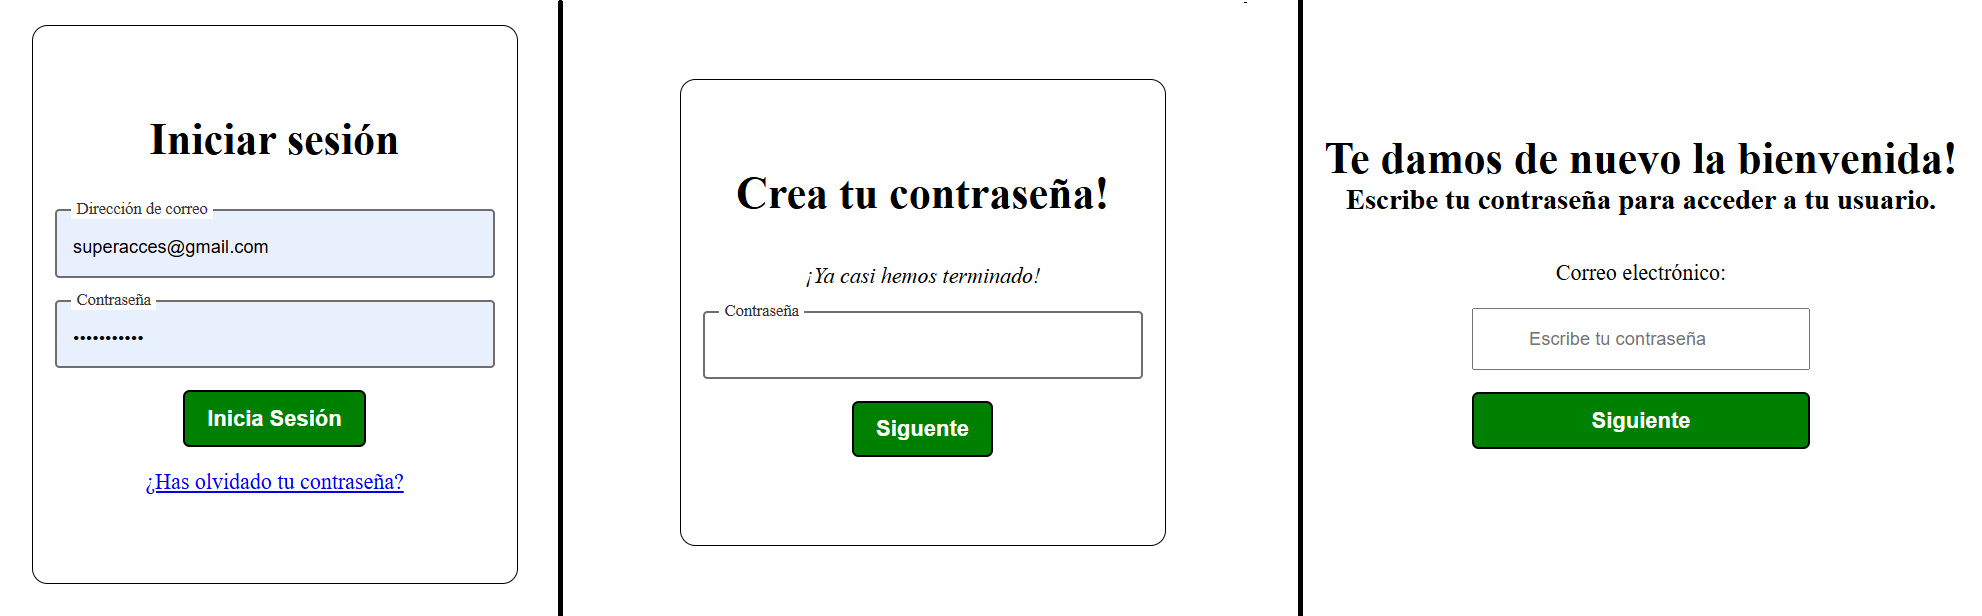
\includegraphics[width=1\textwidth]{img/figPaginesQueExpedeixenJWT.png}
		
		\label{fig:figPaginesQueExpedeixenJWT} 
	\end{figure}
	\FloatBarrier
	
	
	
\textit{NOTA: En este trabajo no implementaremos cookies ya que implica configuración extra tanto en el cliente como en el servidor. Vamos a guardar el token en el cliente en el localStorage (que es, de hecho, una práctica habitual en aplicaciones que no requieren un alto grado de seguridad). También hay que mencionar sobre que existe un debate para ver si en ese logIn el token de acceso recién generado en el servidor se debe mandar al cliente en el body de la respuesta de la solicitud POST \textit{o bien} en la header ``Authorization''. Sin embargo, es práctica común mandarlo en el body. Nótese, que para el paso inverso (cliente a servidor) sí debe mandarse en el Heather ``Authorization'' con el preámbulo ``Bearer '' seguido del token. }
	
	
	
	\subsection{Validación de datos (Formularios entrada)}
	\label{sec:validacioDadesFRONT}
	
	\textit{NOTA: Los datos validados en el front-end siguen las mismas expresiones regulares y restricciones que las validaciones hechas en el back-end (ver sección \ref{sec:validacioDadesBACK}).}
	
	\textbf{TO DO FER-HO}
	
	\subsection{Diseño (UX/UI): páginas publicas}
	\label{sec:disenyoPublicas}
	\textbf{TO DO FER-HO: parlar disseny responsive}
	
	\subsection{Diseño (UX/UI): páginas privadas}
	\label{sec:disenyoResponsivePrivadas}
	
	\subsubsection{Diseño del dashboard}
	
	Parte del diseño del dashboard es un reaprovechamiento del figma y del código HTML y CSS creado para el proyecto final de la asignatura de desarrollo de interfaces, concretamente, de una página donde se explicaban diferencias entre frameworks de front-end que el lector puede consultar  	\href{https://blackcub3s.github.io/proyectoDesarrolloInterfaces/FrontEnd.html}{aquí} para ver la semilla del diseño original.
	
	Esa página fue diseñada y programada por mí de forma íntegra, desde cero con CSS y HTML (a excepción de la Footer que la hizo mi compañero de grupo, dado que era un proyecto grupal). De la parte del footer no se ha aprovechado HTML ni CSS porque el código de la misma no fue de mi autoría, así que se ha optado por un diseño distinto.
	
	El motivo del reaprovechamiento del código es que era imposible asegurar una firma visual distintiva y un aspecto profesional con un diseño desde cero en el poco tiempo para hacer el proyecto. Para hacer la página original, fueron dedicadas muchas, \textit{muchísimas} horas por mi parte: una barbaridad de hecho, así que me sabía mal no reutilizarlo. Además, lo bueno de la reutilización es que se ha podido mejorar la página inicial con dos aspectos que en la asignatura de interfaces NO se pudieron cubrir por los requisitos de la misma:
	
	\vspace{-.8em}
	\begin{itemize}
		\setlength{\itemsep}{-.2em}
		\item \textbf{Diseño responsive}: la página original \texttt{frontEnd.html} del proyecto de interfaces no podía ser responsive mientras que \texttt{dashboard} sí lo es\footnote{en la medida de lo posible, dado que no todas las librerías admiten responsividad: por ejemplo, chart.js no lo es.}.
		\item \textbf{Persistencia de datos}: las vistas de la página del dashboard permiten visualizar datos extraídos de una base de datos de mongoDB.
	\end{itemize}
	
	\noindent Después de esta aclaración vamos a pasar a explicar las secciones del \texttt{dashboard} y de su diseño.
	
	
	
	\noindent \textbf{SECCIÓN 0 (S0): barra de navegación y botón de cierre de sesión}
	\hrule
	\vspace{.5em}
	
	Esta sección incorpora el botón de cierre de sesión (que elimina el token de acceso, en realidad, como ya se ha visto en la sección \ref{sec:tancarSessioBotoExplicacio}) y la barra de navegación que conseguirá redirigir a ubicaciones distintas en función de si se es usuario (permisos=1) o superusuario (permisos=2). También muestra links a páginas que nos permiten ver los tickets del usuario (si los tiene descargados), sus datos en una tabla y una página para contactar con nosotros (ver figuras \ref{fig:barranavegaciodashboardpermisos1}, \ref{fig:barranavegaciodashboardpermisos1dropdown} y \ref{fig:detalleNavbarDesplegadaCodi}).
	
	Además se ha utilizado un sistema (figura \ref{fig:linkAhover})para conseguir que al hacer hover en cada link cambie su color a gris y aparezca una línea por debajo con una transición suave (automatizando las propiedades\textit{border-bottom} y \textit{color}) . Se ha tenido especial cuidado en que el añadir la línea debajo NO desplace el resto de la página hacia abajo. Para evitarlo todos los links tienen en realidad una línea por debajo del mismo color del fondo, que solo cambia de color al pasar por encima. Hay muchas líneas de código para conseguirlo y redirigimos al lector al github para verlas (nótese el uso de selectores descendientes, por norma: \href{https://github.com/blackcub3s/mercApp/blob/main/APP%20WEB/__frontend__produccio__/app/css/dashboard/navFooter.css}{link a navFooter.css})
	
	\FloatBarrier
	\setlength{\abovecaptionskip}{3pt}
	\begin{figure}[H]
		\centering
		\caption{Barra de navegación del usuario de permisos=1 con sus 4 elementos}
		
\includegraphics[width=1\linewidth]{img/barraNavegacioDashboardPERMISOS1}

		\label{fig:barranavegaciodashboardpermisos1}
	\end{figure}
	\FloatBarrier
	
	Dentro de la sección servicios hay un desplegable o ``dropdown" que nos permite llegar a las distintas secciones del dashboard: el ``inflalyzer'', el ``categorizer'' y el ``intervalizer''.
	
	\FloatBarrier
	\setlength{\belowcaptionskip}{3pt}
	\begin{figure}[H]
		\centering
		\caption{Detalle barra de navegación con el drop-down desplegado.}
		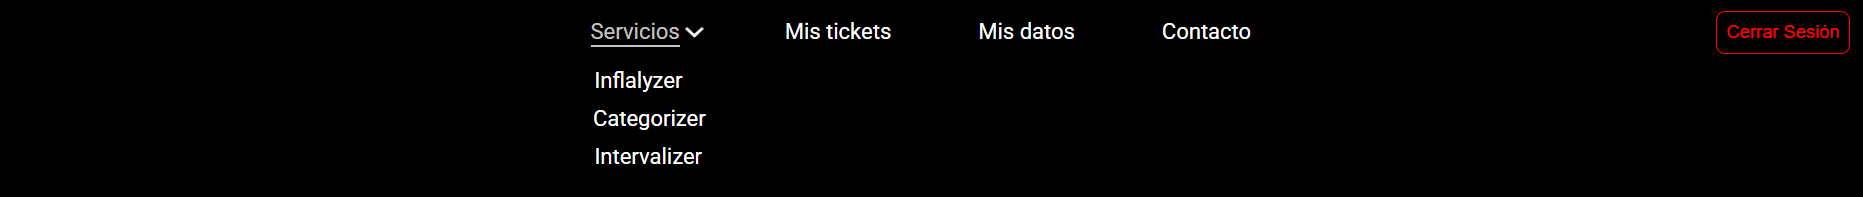
\includegraphics[width=1\linewidth]{img/barraNavegacioDashboardPERMISOS1dropDown}
		
		\label{fig:barranavegaciodashboardpermisos1dropdown}
	\end{figure}
	\FloatBarrier
	
	
	\FloatBarrier
	\setlength{\belowcaptionskip}{0pt}
	\begin{figure}[H]
		\centering
		\caption{Detalle del código que hizo posible el drop-down del menú. Cada elemento drop down se ha animado mediante animate.css definiendo distintas duraciones de la animación \textit{fadeInDown} para conseguir un efecto persiana. El uso del selector descendiente y el no abuso de los IDs a menos que sea necesario es una metodología seguida a lo largo del diseño del dashboard.}
		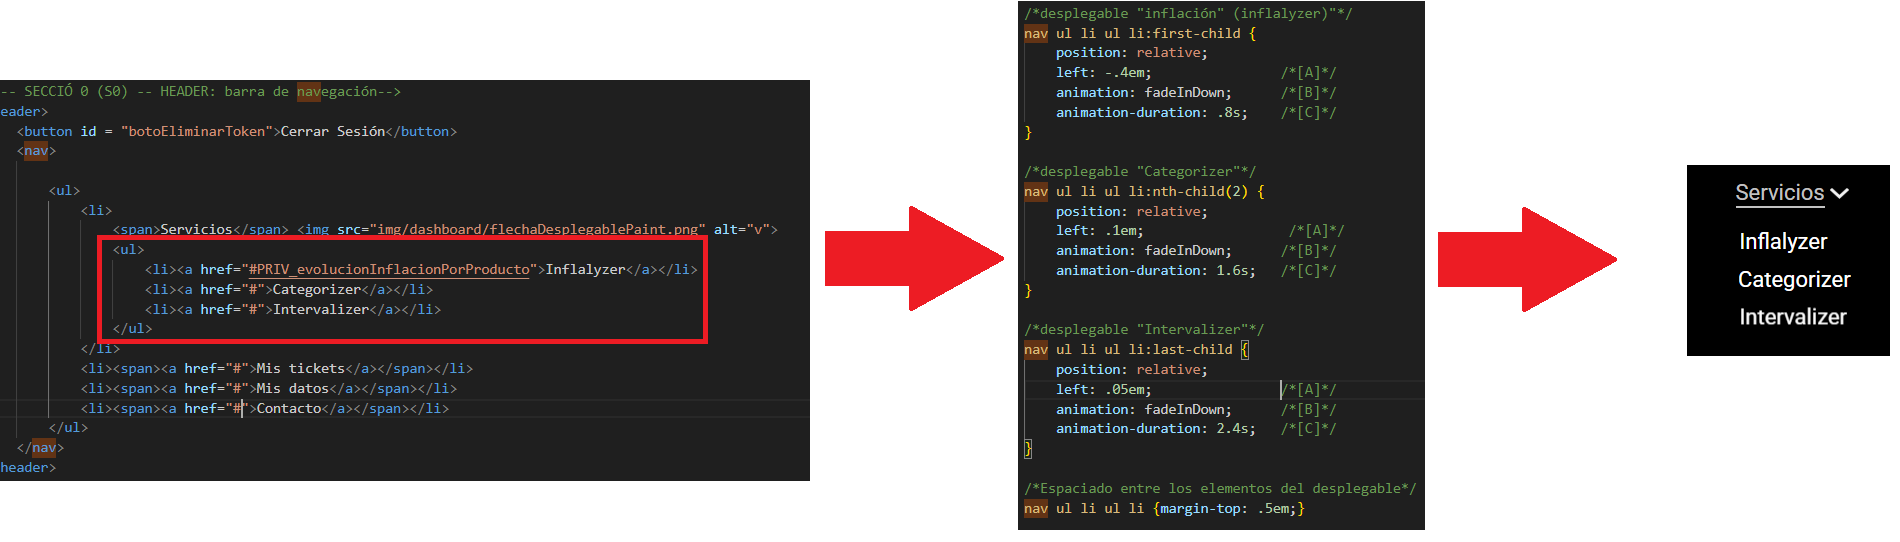
\includegraphics[width=1\linewidth]{img/navBarDesplegadaMakingOfPermisos1.png}

		\label{fig:detalleNavbarDesplegadaCodi}
	\end{figure}
	\FloatBarrier
	
	\FloatBarrier
	\begin{figure}[H]
		\centering
		\caption{Transiciones suaves de propiedades \textit{border-bottom }y \textit{color} al hacer hover en los spans que envuelven los links tanto en la barra de navegación como en la footer.}
		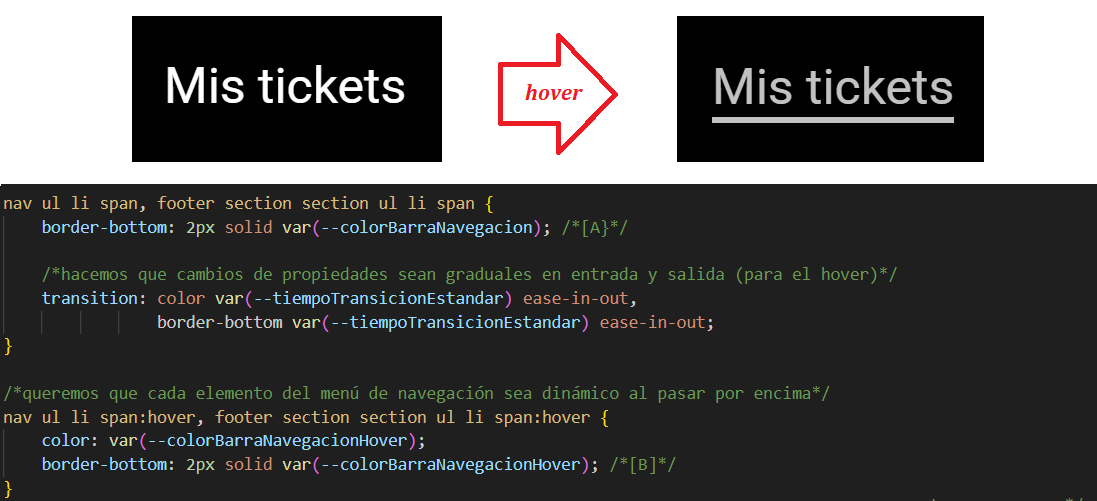
\includegraphics[width=1\linewidth]{img/linkAhover.png}
		
		\label{fig:linkAhover}
	\end{figure}
	\FloatBarrier
	
	
	
	
	
	
	
	
	\noindent \textbf{SECCIÓN 1 (S1): presentación Dashboard}
	\hrule
	\vspace{.5em}
	
	Esta sección simplemente muestra un gradiente lineal que transiciona del negro de la barra de navegación hacia el azul claro que es colindante a la barra roja. Para hacerlo se ha hecho mediante un doble gradiente lineal. También se ha usado la clase fadeIn de animate.css para hacer que aparezca con un fundido de entrada al cargar o recargar la página. Podéis ver la figura que muestra el código en \ref{fig:S1FrontMakeOf}.
	
	\FloatBarrier
	\setlength{\belowcaptionskip}{3pt}
	\begin{figure}[H]
		\centering
		\caption{De izquierda a derecha: código HTML, codigo CSS y el resultado final de la vista de esa sección}
		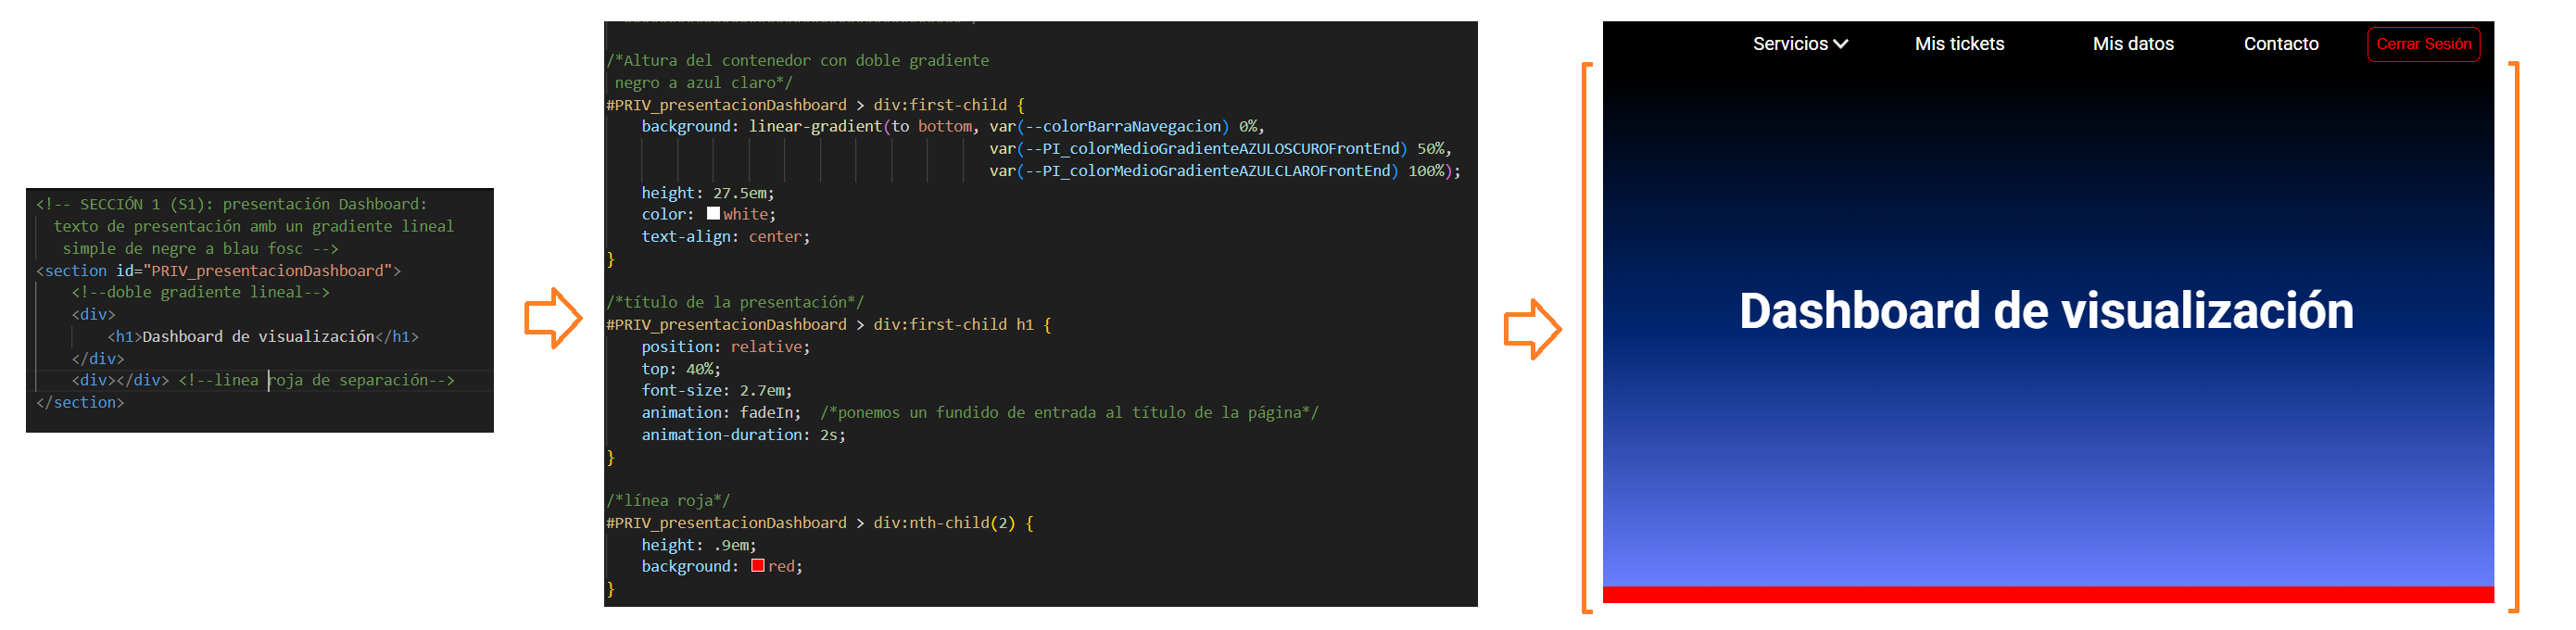
\includegraphics[width=1\linewidth]{img/S1FrontMakeOf.png}
		
		
		\label{fig:S1FrontMakeOf}
	\end{figure}
	\FloatBarrier
	
	
	
	
	\noindent \textbf{SECCIÓN 2 (S2): características de la aplicación mercApp:}
	\hrule
	\vspace{.5em}
	
	Esta sección contiene tres ``cards'' que resumen los servicios que ofrece el resto del dashboard (inflación por producto, gastos por categoría y gastos por ventana temporal): también incorporan los datos más relevantes de los tikets de cada usuario, que se extraen también de la BBDD (ver detalle figura \ref{fig:s2caracteristiquesmercapp}). El lector puede consultar el fichero \href{https://github.com/blackcub3s/mercApp/blob/main/APP%20WEB/__frontend__produccio__/app/css/dashboard/estils.css}{estils.css} todos los selectores css descendientes que empiezan por el id con el que encabezamos el section de esa parte (id \textit{PRIV\_caracteristicasDashboard}).

	
	De estas cards hay tres aspectos a destacar: En \textit{primer lugar}, se ha vigilado en que sigan exactamente la proporción áurea. Al crearlas se ha definido la propiedad CSS \textit{aspect-ratio} (\href{https://github.com/blackcub3s/mercApp/blob/663360ea63eafd38c1fa052e7a994e22d7f0a5f6/APP%20WEB/__frontend__produccio__/app/css/dashboard/estils.css#L80}{ver en GitHub} para que la relación de aspecto ancho-alto de cada una de ellas sea exactamente de 1 a 1.618 \cite{wikiPropAurea}. De este modo, creamos un rectángulo agradable a la vista para poder presentar los primeros datos del resumen de los tickets al usuario. \textit{En segundo lugar}, en cada una de las cards se ha usado un gradiente lineal vertical mediante la propiedad CSS \textit{background} (\href{https://github.com/blackcub3s/mercApp/blob/663360ea63eafd38c1fa052e7a994e22d7f0a5f6/APP%20WEB/__frontend__produccio__/app/css/dashboard/estils.css#L85}{ver línea}) que hemos utilizado también para cambiar dinámicamente ambos colores del gradiente al hacer hover (\href{https://github.com/blackcub3s/mercApp/blob/663360ea63eafd38c1fa052e7a994e22d7f0a5f6/APP%20WEB/__frontend__produccio__/app/css/dashboard/estils.css#L126}{ver línea}). En esos casos, además el hover altera también el \textit{box-shadow} definido en esta \href{https://github.com/blackcub3s/mercApp/blob/663360ea63eafd38c1fa052e7a994e22d7f0a5f6/APP%20WEB/__frontend__produccio__/app/css/dashboard/estils.css#L84}{línea} y lo modifica a otro valor (\href{https://github.com/blackcub3s/mercApp/blob/663360ea63eafd38c1fa052e7a994e22d7f0a5f6/APP%20WEB/__frontend__produccio__/app/css/dashboard/estils.css#L125}{en esta}). El resultado de esta programación es el que se puede ver en la figura \ref{fig:cardCaracteristicaAbansDespres}. También se han definido automatizaciones de la propiedad \textit{transform} para las imágenes de dentro de las cards, para hacer que aumenten de tamaño al posarnos con el ratón por encima (\href{https://github.com/blackcub3s/mercApp/blob/663360ea63eafd38c1fa052e7a994e22d7f0a5f6/APP%20WEB/__frontend__produccio__/app/css/dashboard/estils.css#L106-L108}{detalle líneas}).
	
	Finalmente, merece la pena mencionar que mediante wow.js se ha conseguido crear las animaciones de animate.css (como las que se usaron en la sección 0, ver captura previa \ref{fig:detalleNavbarDesplegadaCodi}) de modo que en lugar de que aparezcan con un temporizador desde la carga de la página como nos permite la librería animate.css, sino que aparezcan con un temporizador desde que hacemos scroll a la sección que las incluye.
	
	Así las cosas, las propiedades que nos define animate.css en este caso no las hemos escrito en el CSS sino que lo hemos hecho en el propio HTML de acuerdo con el requerimiento de la librería \textit{wow.js}. De este modo al hacer scroll a la sección, la card de la izquierda aparecerá por la izquierda (fadeInLeft,  \href{https://github.com/blackcub3s/mercApp/blob/663360ea63eafd38c1fa052e7a994e22d7f0a5f6/APP%20WEB/__frontend__produccio__/app/dashboard.html#L130}{link}), la del medido de abajo (fadeInUp,  \href{https://github.com/blackcub3s/mercApp/blob/663360ea63eafd38c1fa052e7a994e22d7f0a5f6/APP%20WEB/__frontend__produccio__/app/dashboard.html#L153}{link}) y la de la derecha de esa misma dirección (fadeInRight,  \href{https://github.com/blackcub3s/mercApp/blob/663360ea63eafd38c1fa052e7a994e22d7f0a5f6/APP%20WEB/__frontend__produccio__/app/dashboard.html#L173}{link}). Una ves hecho esto se ajustó la duración y el \textit{delay} de cada propiedad mediante atributos en esas mismas líneas del HTML.
	
	
	\FloatBarrier
	\begin{figure}[H]
		\centering
		\caption{Detalle de la sección con las tres cards: características resumidas del dashboard. Los textos en color son placeholders para lo que se extraerá de la BBDD.}
		\label{fig:s2caracteristiquesmercapp}
		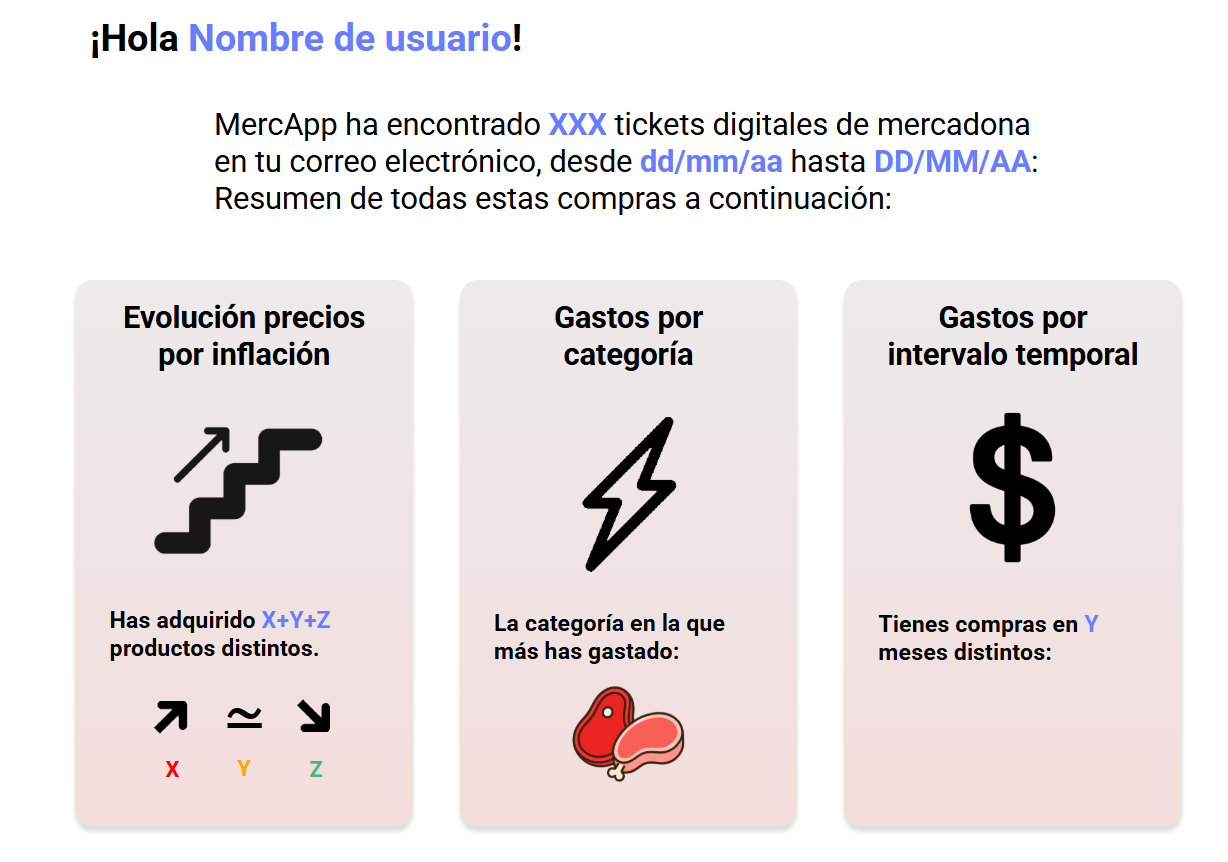
\includegraphics[width=1\linewidth]{img/s2CaracteristiquesMercApp.png}
	\end{figure}
	\FloatBarrier
	
		\FloatBarrier
	\begin{figure}[H]
		\centering
		\caption{Detalle del impacto que tiene la automatización de \textit{box-shadow} y \textit{background} al hacer hover encima de las cards.}
		\label{fig:cardCaracteristicaAbansDespres}
		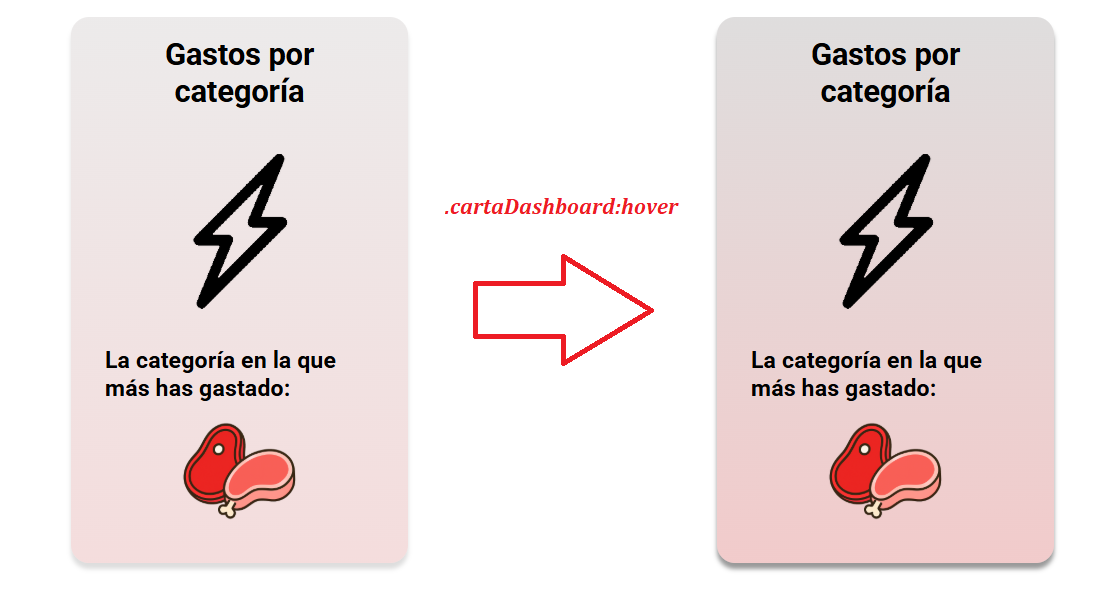
\includegraphics[width=1\linewidth]{img/cardCaracteristicaAbansDespres.png}
	\end{figure}
	\FloatBarrier
	
	
	
	\noindent \textbf{SECCIÓN 3 (S3): ``inflalyzer'' (sin swiper: ¡esta vez hecho a mano!) }
	\hrule
	\vspace{.5em}
	En la página original de la que hemos derivado parte del dashboard (\href{https://blackcub3s.github.io/proyectoDesarrolloInterfaces/FrontEnd.html}{link}) utilizamos la librería swiper para cambiar entre imágenes de una galería mediante clicks en unos paginadores (si no podéis ver la web, podéis ver detalle en figura \ref{fig:swiperFront} del anexo). Tratar de reutilizarlo para nuestro caso fue imposible: ahora no tenemos solo imágenes a ir variando con los paginadores, sino que tenemos una tabla entera a poner dentro de esos paginadores. Swiper esto no lo podía manejar.
	
	Así las cosas hubo que crear un swiper manualmente para poder albergar una tabla dentro del paginador (ver figura \ref{fig:imatgeSwiperCustom}). Este ``swiper'' artesanal, se creó tomando los mismos iconos de swiper, eliminado el canal alpha del fondo, cambiando su color de azul a rojo y definiendo eventos de click a las imágenes que conforman esas flechitas.
	
	\FloatBarrier
	\begin{figure}[H]
		\centering
		\caption{Detalle de la parte superior del intervalizer: obsérvese el paginador creado manualmente}
		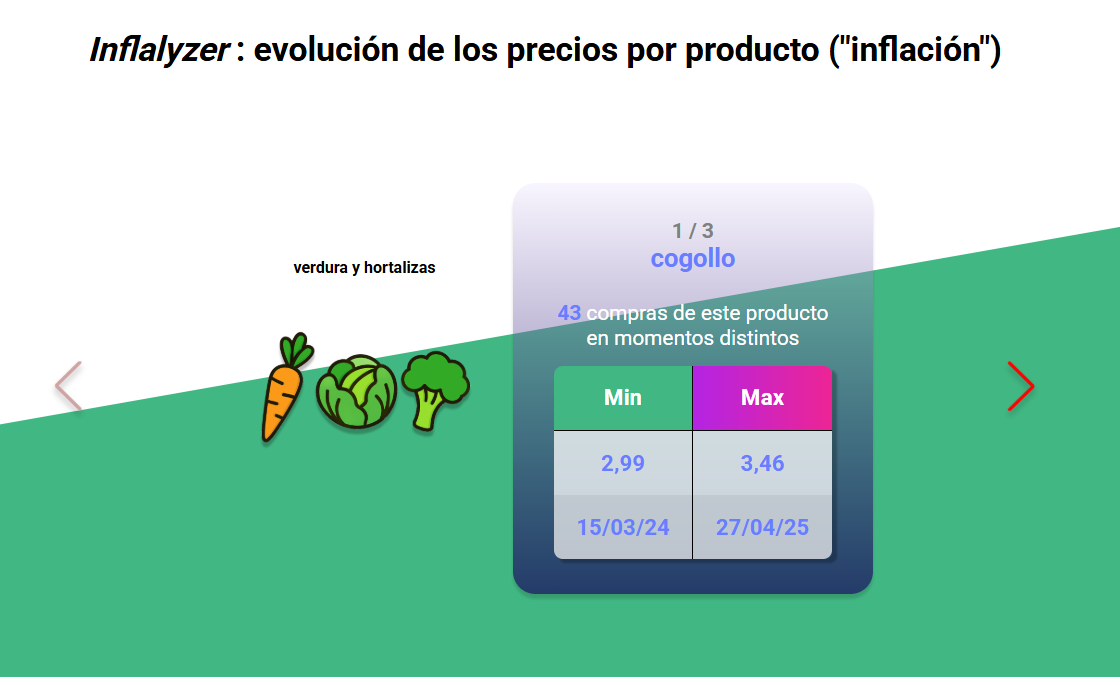
\includegraphics[width=1\linewidth]{img/imatgeSwiperCustom.png}
		\label{fig:imatgeSwiperCustom}
	\end{figure}
	\FloatBarrier
	
	A nivel de UX/UI el paginador de la figura \ref{fig:imatgeSwiperCustom} ha seguido los mismos principios. En este caso, hay un par de cosas destacables. El uso de imágenes customizadas para los botones de paginación nos ha habilitado para usar \textit{hover} afectando la propiedad \textit{drop-shadow} de la imagen del paginador, para así aprovechar los contornos del mismo hacer transform y dar la sensación de profundidad \textbf{combinando la sombra con el incremento de tamaño} (ver imagen \ref{fig:paginadorscustom}).
	

	\FloatBarrier
	\begin{figure}[H]
		\centering
		\caption{Paginadores para moverse hacia productos con más frecuencia de compra: a la izquierda sin hover (drop-shadow difuso y poco visible) y con hover a la derecha de la captura (drop-shadow con menos difusión de imagen y ligeramente desplazado hacia abajo).}
		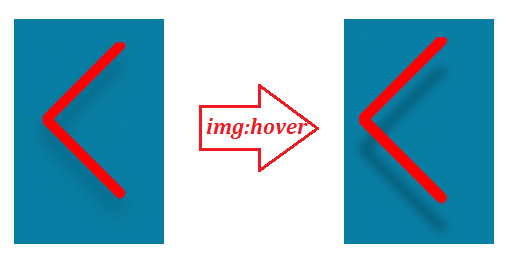
\includegraphics[width=1\linewidth]{img/paginadorsCustom}

		\label{fig:paginadorscustom}
	\end{figure}
	\FloatBarrier
	
	Asimismo, cuando llegamos al final del listado de productos del usuario, sea por la izquierda o la derecha, se cargan unas imágenes difuminadas que además con JavaScript no permitimos que traten de acceder a ningún dato (\href{https://github.com/blackcub3s/mercApp/blob/main/APP%20WEB/__frontend__produccio__/app/img/dashboard/paginadorEsqDifuminat.png}{ver detalle}).
	
	El CSS de la imagen \ref{fig:imatgeSwiperCustom} está disponible en este rango de líneas de GitHub \href{https://github.com/blackcub3s/mercApp/blob/4ddc34194763af7a246ffabb14146ad9b4b2c5db/APP%20WEB/__frontend__produccio__/app/css/dashboard/estils.css#L155}{link}. Para observar el JavaScript de la paginación se puede visualizar el apartado \ref{sec:paginadorJavascriptArquitectura}.
	
	
	
	
	\noindent \textbf{SECCIÓN 4 (S4): ``categoryzer''}
	\hrule
	\vspace{.5em}
	
	\textbf{TO DO}
	
	
	\noindent \textbf{SECCIÓN 5 (S5): ``intervalizer''}
	\hrule
	\vspace{.5em}
	
	\textbf{TO DO}
	
	\subsubsection{Diseño del ``pas4''}
	
	\subsection{Arquitectura (JavaScript): páginas privadas}
	
	\subsubsection{Arquitectura del dashboard}
	\label{sec:paginadorJavascriptArquitectura}
	
	El \textbf{paginador customizado} que vimos en la figura \ref{fig:imatgeSwiperCustom} requiere JavaScript. El código que lo consigue orquestrar se encuentra en el archivo \href{https://github.com/blackcub3s/mercApp/blob/main/APP%20WEB/__frontend__produccio__/app/js/dashboard/paginadorInflacio.js}{paginadorInflacio.js}.
	
	\textbf{TO DO PARLAR DEL GRAFIC D'INFLACIO I DEL SEU JAVASCRIPT (continuacio inflalyzer)}
	
	\textbf{TO DO PARLAR DEL DIAGRAMA DE SECTORS I DEL JS}
	
	\textbf{TO DO PARLAR DEL CATEGORIZER I DEL JS}
	
	\textbf{TO DO PARLAR DEL INTERVALIZER I DEL JS}
	
	
	
	La extracción de datos de la base de datos se hace principalmente desde \href{	https://github.com/blackcub3s/mercApp/blob/main/APP%20WEB/__frontend__produccio__/app/js/dashboard/extractorDadesPersistencia_enCarregarPagina.js}{extractorDadesPersistencia\_enCarregarPagina.js}
	
	\textbf{HI HA MES ARXIUS DE PERSISTENCIA? REAVALUAHO??}
	
	
	\subsubsection{Arquitectura pas4: llamada a google API client}
	\label{sec:pas4googleAPIclient}
	
	Para hacer esta parte es importante mencionar que tenemos que configurar la consola de google cloud (\href{https://console.cloud.google.com/}{https://console.cloud.google.com/}). En última instancia tenemos que obtener el \textbf{Client ID} que identifique nuestra web en relación a Google Cloud. Todos estos pasos se indican en una sección a parte que recomendamos al lector que lea, porque ha supuesto varios días de trabajo \ref{sec:desarrolloCloudGoogleApi}.
	
	Una vez obtenido este id, se permitá que los usuarios de nuestro sitio web (en el \href{https://github.com/blackcub3s/mercApp/blob/main/APP%20WEB/__frontend__produccio__/app/pas4_concedirAccesGmail.html}{\texttt{pas4\_concedirAccesGmail.html}}) puedan descargarse sus tickets digitales del correo gmail personal \textit{hacia} la carpeta de descargas de su ordenador, mediante uso de JavaScript puro. Se utilizará el remitente de la dirección de correo electrónico desde la que Mercadona nos manda los tickets digitales para poder filtrar los correos y descargar sus pdfs. La dirección es: \textbf{ticket\_digital@mail.mercadona.com}.

	
	
	La extracción de tickets \underline{no se puede hacer en local con javascript} porque las políticas de seguridad del navegadorno permiten scripts llamando a API de google sin HTTPS. Debe hacerse, por lo tanto, desde un script en remoto, en un dominio autorizado en internet, con protocolo HTTPS y autorizado desde la configuración de la consola de google (Que ya hemos hecho). Para ello he creado este repositorio para hacer descargas de tickets (\href{https://github.com/blackcub3s/mercAppAuxPas4/}{repo mrcAppAuxPas4}).
	
	De este repo, el único archivo que usaremos en \texttt{pas4\_concedirAccesGmail} corriendo en localhost será este (\href{https://github.com/blackcub3s/mercAppAuxPas4/blob/main/js/scriptExtraccio.js}{scriptExtraccio.js}). Para poder correr el script usaremos su ruta en github pages (no el del repositorio github, sino el que se carga en la página de github pages que hace el deploy de este mismo repositorio). Esto lo haremos haciendo uso de la URL del script, pero sin el grupo ``blob/main''. Luego lo cargaremos en \texttt{pas4\_concedirAccesGmail.html} como si fuera servido de una CDN externa\footnote{Solo que la CDN la hemos creado expresamente.}:
	
	\begin{lstlisting}[language=java, basicstyle=\ttfamily\small]
<script src="https://blackcub3s.github.io/
             mercAppAuxPas4/js/scriptExtraccio.js"></script>
	\end{lstlisting}
	
	



		
	
		
	\subsection{arquitectura dashboard: llamada fetch inicial a back-end mongoDB y posteriores a localStorage}
	\label{sec:dashboardFetchLocalStorage}
	\textbf{TO DO FER-HO}
	
	
	\subsection{Diseño de iconos}
	
	\subsubsection{Áreas de producto}
	
	Los iconos de las 8 áreas en las que hemos decidido clasificar los productos de Mercadona (véase apartado \ref{sec:requisitosAplicacion}, requisito C) se han generado mediante inteligencia artificial generativa y se han editado posteriormente con Gimp para eliminar el fondo y generar transparencia en el mismo (ver \href{https://github.com/blackcub3s/mercApp/tree/main/creacioIconos/categoriesProductes}{carpeta GitHub}).
	
	
	En la figura \ref{fig:eliminocanalalpha}, podemos ver la creación de uno de los iconos con chatGPT y la eliminación posterior del fondo con GIMP. 
	
	Hay que mencionar, sin embargo, que el procedimiento de GIMP ahí mostrado no permite conseguir una transparencia pura del fondo. Para conseguirlo en algunos iconos es indispensable usar otro procedimiento que involucra más pasos pero que nos permite asegurarnos que se elimina por completo el canal alpha del fondo (ver figura \ref{fig:eliminocanalalphaCOMPLEX}). La utilidad de ese último procedimiento en relación al anterior puede verse en la figura \ref{fig:ventatjaProcedComplexVSsimple} donde comparamos la aplicación de ambos procedimientos al mismo icono.


	
	
	
	
\FloatBarrier
\setlength{\belowcaptionskip}{3pt}
\begin{figure}[H]
	\centering
	\caption{Se ha pedido a chat gpt la creación del icono de verduras y hortalizas. Chat gpt no elimina el canal alpha del fondo automáticamente, así que hemos tenido que tomar la imagen saliente (A), pasarla por Gimp y exportarla  sin el fondo (B). Para hacerlo dentro de gimp seleccionamos el color blanco con la herramienta de selección (varita mágica) y seguimos la ruta \textit{capa} $\rightarrow$ \textit{transparencia} $\rightarrow$ \textit{color a alpha}.}
	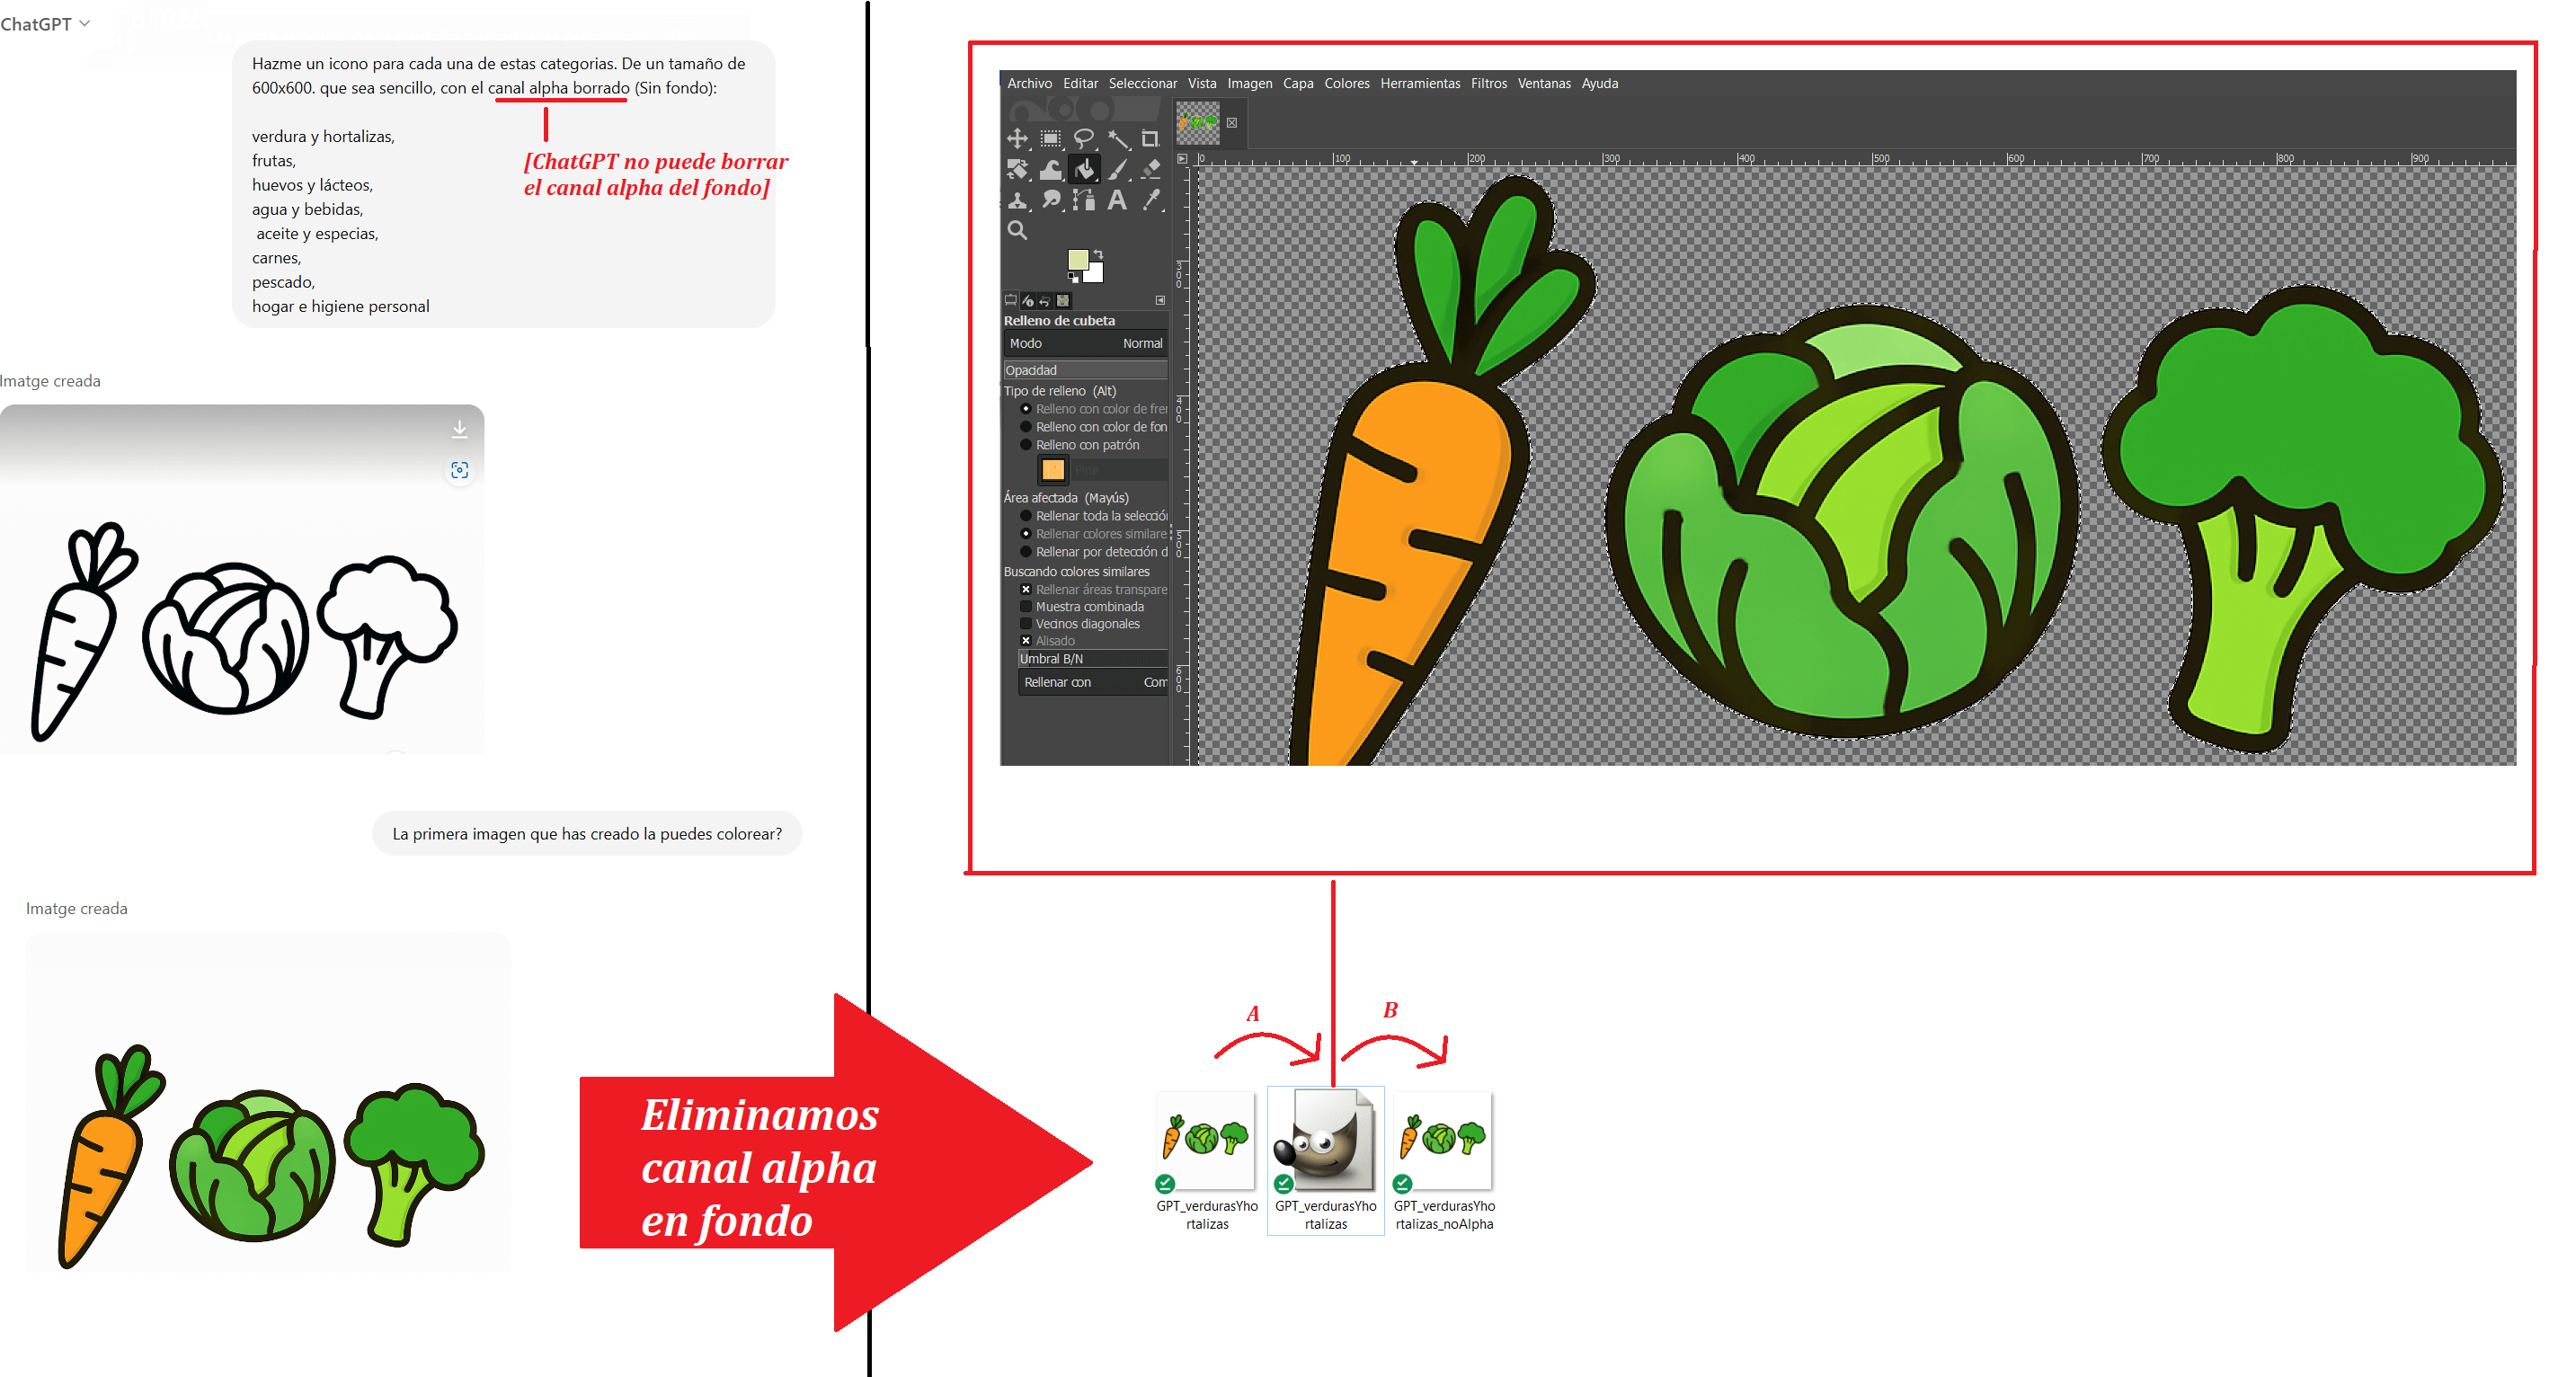
\includegraphics[width=1\linewidth]{img/eliminoCanalAlpha}


	\label{fig:eliminocanalalpha}
\end{figure}
\FloatBarrier


\FloatBarrier
\setlength{\belowcaptionskip}{3pt}
\begin{figure}[H]
	\centering
	\caption{En determinados casos no es suficiente con la estrategia sencilla del paso anterior y debemos seguir este procedimiento, que incluye el uso de la varita mágica, y de los pasos \textit{Seleccionar} $\rightarrow$ \textit{invertir} (invertir selección) y \textit{Ctrl + X} seguido de \textit{Ctrl + V} como mostramos en la figura.} 
	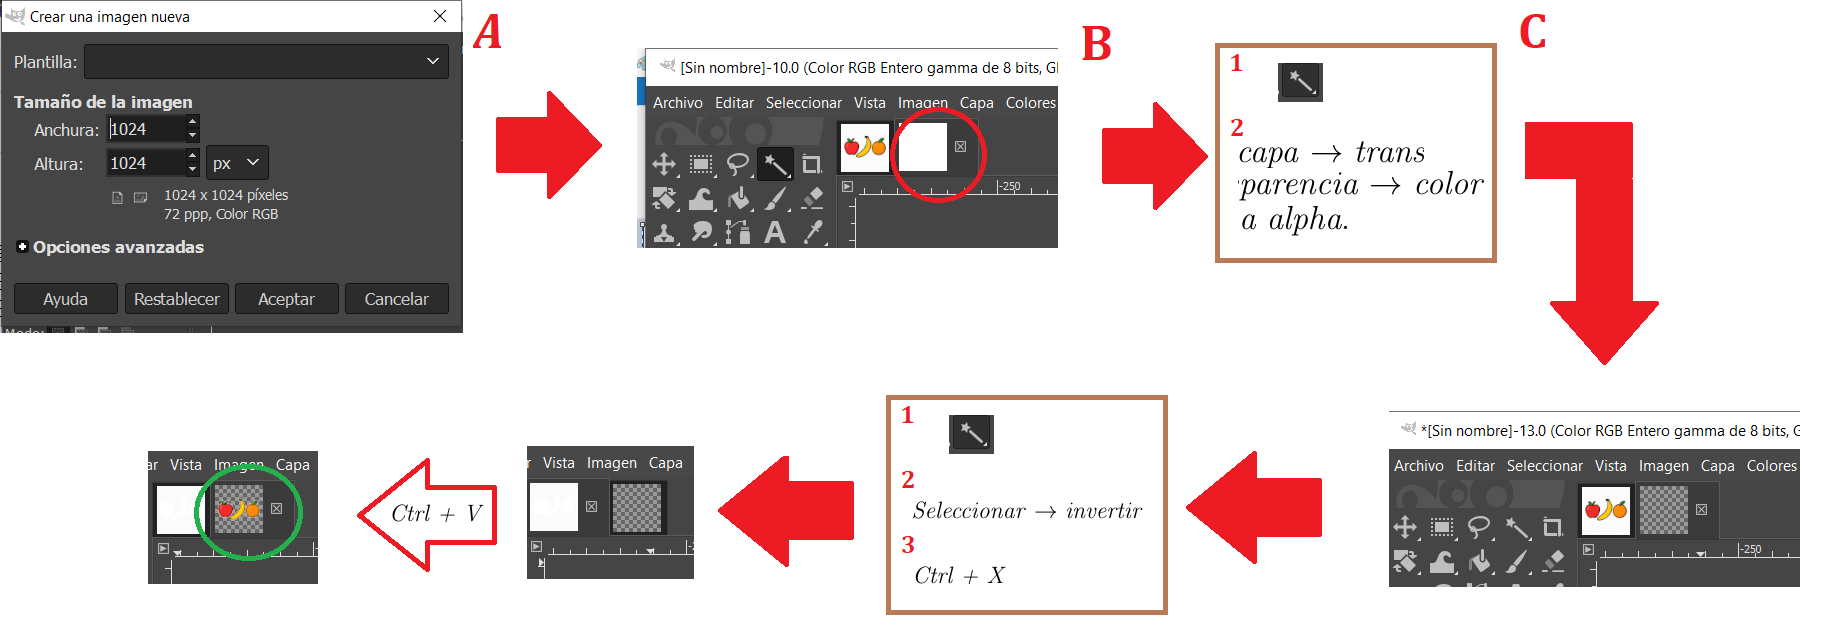
\includegraphics[width=1\linewidth]{img/eliminoCanalAlphaCOMPLEX.png}

	
	\label{fig:eliminocanalalphaCOMPLEX}
\end{figure}
\FloatBarrier



\FloatBarrier
\setlength{\belowcaptionskip}{3pt}
\begin{figure}[H]
	\centering
	\caption{El procedimiento de Gimp mostrado en la figura \ref{fig:eliminocanalalpha} genera un icono que en contexto se verá como la imagen de la izquierda: la card central del dashboard mostraría un icono con bordes rectangulares no intencionados. El procedimiento de la figura \ref{fig:eliminocanalalphaCOMPLEX}, en cambio, nos da la imagen de la derecha que no tiene fondo alguno y permite que el icono se asente a la perfección en la card.}
	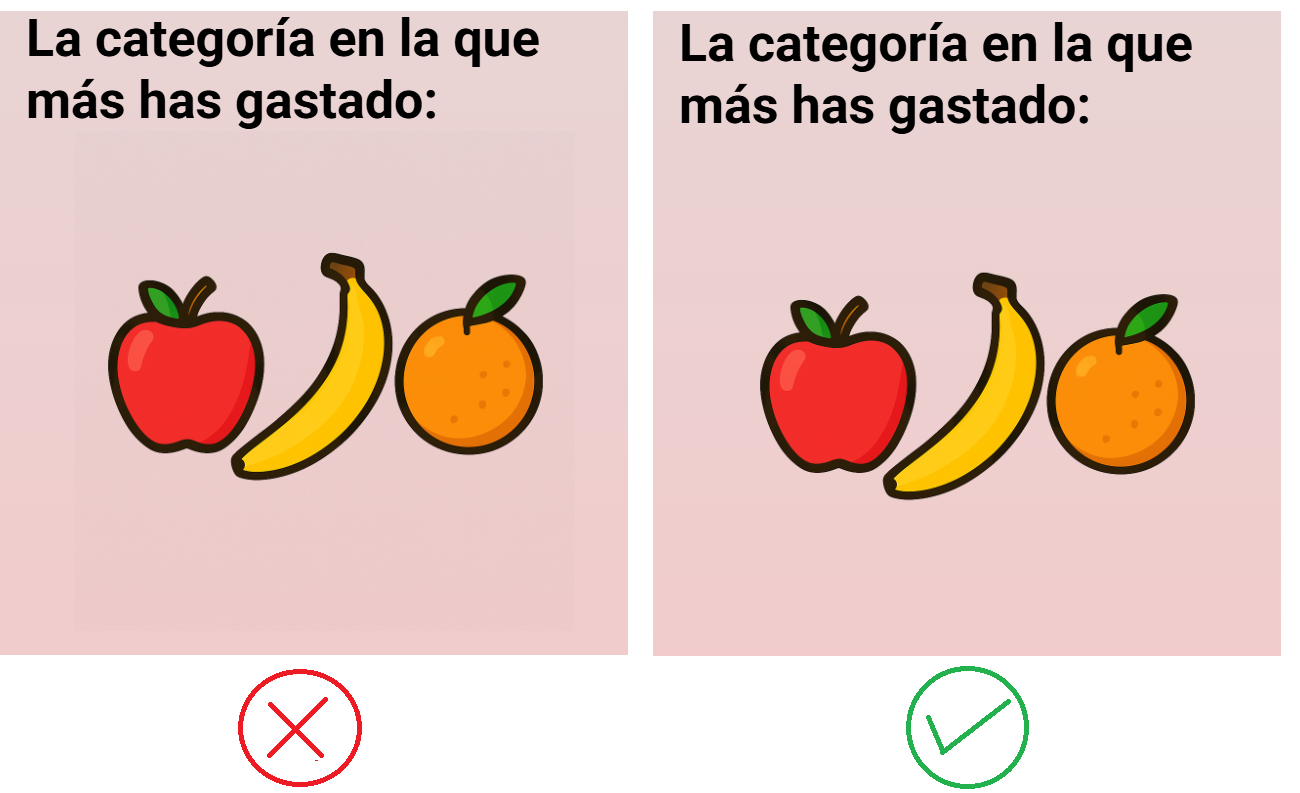
\includegraphics[width=1\linewidth]{img/ventatjaProcedComplexVSsimple.png}

	
	\label{fig:ventatjaProcedComplexVSsimple}
\end{figure}
\FloatBarrier
	
	
	\subsubsection{Icono mercApp pequeño}
	\label{sec:iconoMercappPetitMEMORIAPPAL}
	Este icono también se ha pedido a la IA y se ha editado posteriormente, mostrando el icono grande para que lo usase. Se puede ver en el anexo \ref{sec:edicionMercAppIconoPequenyo} el proceso completo que también involucra edición en gimp . Pero el proceso resumido viene a ser el de la figura: \ref{fig:mercappResumit}.
		
		
	\FloatBarrier
	\setlength{\belowcaptionskip}{3pt}
	\begin{figure}[H]
		\centering
		\caption{El prompt pasado a ChatGPT para obtener una versión reducida del icono de nuestra APP. Incluso con con typos en el prompt la IA entiende perfectamente lo que necesitamos.}
		
\includegraphics[width=1\linewidth]{img/mercappResumit}
		\label{fig:mercappResumit}
	\end{figure}
	\FloatBarrier
		
		
		
	\section{Desarrollo Cloud: configuración google api client}
	\label{sec:desarrolloCloudGoogleApi}
	
	\noindent NOTA: regresar a apartado \ref{sec:pas4googleAPIclient} una vez comprendido este apartado, si no se ha leido.
	
	Para conseguir que la extracción de tickets funcione en el \textbf{pas4} (sección \ref{sec:pas4googleAPIclient}) es indispensable configurar (\href{https://console.cloud.google.com/}{https://console.cloud.google.com/}). 
	
	Esta configuración es necesaria por varios motivos: El primero, es que tenemos que  obtener el (\textbf{Client ID}) para que se identifique nuestra web en relación a Google Cloud; el segundo, es configurar los ``\textit{scopes}'' que le dicen a Google qué tratamos de conseguir del gmail de los usuarios (aqui lectura de gmails -gmail.readonly-); el tercero, definir un listado de usuarios que permitirán usar nuestra aplicación (durante la fase de desarrollo); y el último, pero no por ello menos importante, la lista de direcciones IP desde las que google deberá permitirnos hacer llamadas a su API.
	
	A continuación explicamos todos los pasos de forma pormenorizada para conseguir hacer todo esto:
	
	
	\noindent \textbf{PASO 1: Crear un nuevo proyecto en la consola}
	\vspace{.2em}
	\hrule
	\vspace{.5em}
	
	Para crear  el nuevo proyecto una vez dentro de la vista general de la consola clicamos encima de MyFirstProject y creamos un proyecto nuevo como vemos en la figura, añadiendo el nombre ``descarregaTicketsGmail'', que será el nombre que le daremos al proyecto (ver figura \ref{fig:googleCloudA}):
	\FloatBarrier
	\setlength{\belowcaptionskip}{3pt}
	\begin{figure}[H]
		\centering
		\caption{Pasos para crear un nuevo proyecto en la consola de google cloud.}
		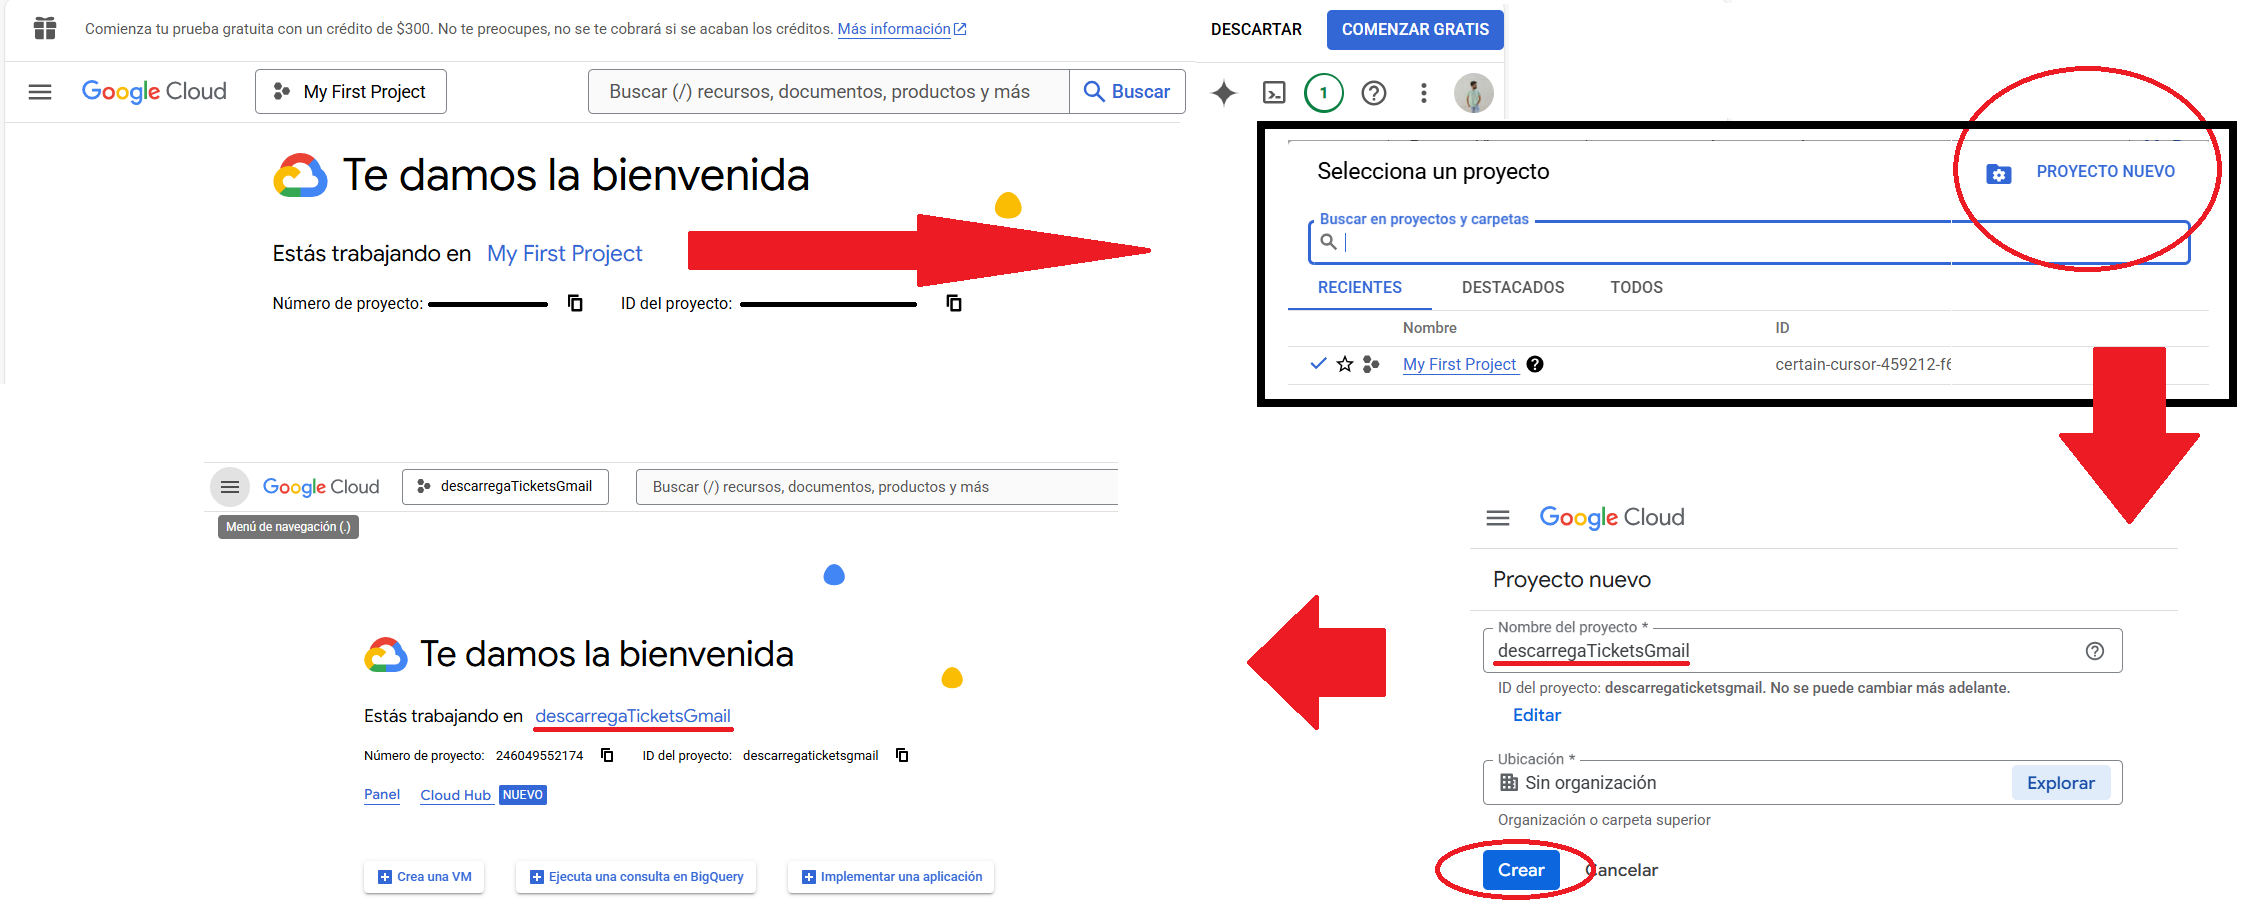
\includegraphics[width=1\linewidth]{img/googleCloudA.png}
		\label{fig:googleCloudA}
	\end{figure}
	\FloatBarrier
	
	
	
	
	
	
	
	
	
	
	
	
	
	\noindent \textbf{PASO 2: Habilitar la Gmail API}
	\vspace{.2em}
	\hrule
	\vspace{.5em}
	
	Para habilitar la API de gmail, que nos permitirá \textbf{ver y manejar datos del inbox de un correo electrónico} (que es la que usaremos para descargar los tickets adjuntos en PDF), debemos entrar en nuestro proyecto recién creado y seguir los menús ``\textit{APIs y servicios}'' $\rightarrow$ \textit{Biblioteca}. Ahí, buscar ``\textit{gmail API}'' y habilitar la Gmail API (figura \ref{fig:googleCloudC}).
	
	\FloatBarrier
	\setlength{\belowcaptionskip}{3pt}
	\begin{figure}[H]
		\centering
		\caption{Como habilitar la Gmail API en nuestro proyecto ``descarregaTicketsGMAIL''}
		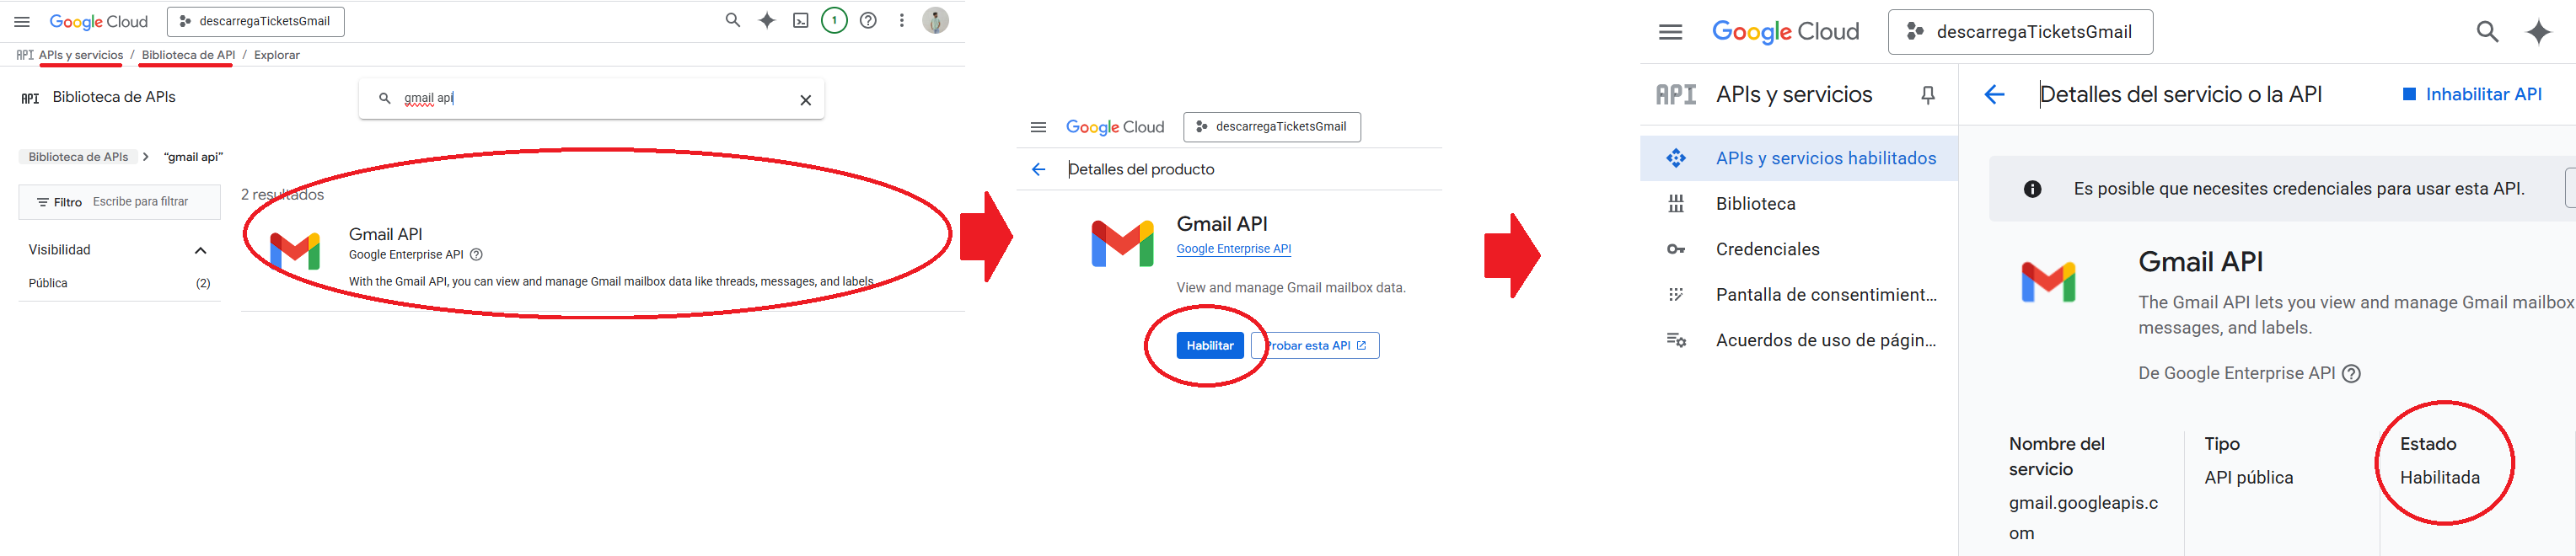
\includegraphics[width=1\linewidth]{img/googleCloudC.png}
		\label{fig:googleCloudC}
	\end{figure}
	\FloatBarrier
	
	\noindent \textbf{PASO 3: Configurar la pantalla de consentimiento OAuth}
	\vspace{.1em}
	\hrule
	\vspace{.5em}
	
	Oauth nos permitirá que los usuarios sean autorizados a servicios de Google como Gmail y, además, también les autenticará para dejar que nuestra aplicación en JavaScript del \texttt{pas4\_concedirAccesGmail.html} pueda acceder a su correo Gmail\footnote{¡Cuidado, no confundir la autenticación y autorización de nuestra aplicación y el manejo de nuestros AccessTokens con la autenticación con Oauth 2.0: esta última es OBLIGATORIA para acceder a los servicios de Google y la controla Google.}.
	
	Análogamente al paso anterior seguimos los menús de la izquierda ``\textit{APIs y servicios} $\rightarrow$ \textit{Pantalla de consentimiento OAuth} (ver figura \ref{fig:googleCloudD}).
	
	\FloatBarrier
	\setlength{\belowcaptionskip}{3pt}
	\begin{figure}[H]
		\centering
		\caption{Habilitación de la pantalla de consentimiento de OAuth: Especificamos el nombre de la aplicación, el correo al que podrán comunicarse los usuarios de la aplicación mercApp del cloud si es necesario, marcamos el radioButton ``usuarios externos'', que hará que puedan utilizar la app en el cloud usuarios sin una extensión de correo vinculada a una organización especifica (si no lo marcásemos, estaríamos limitados a usuarios con una extensión específica de organización y no podríamos usar correos gmail!).}
		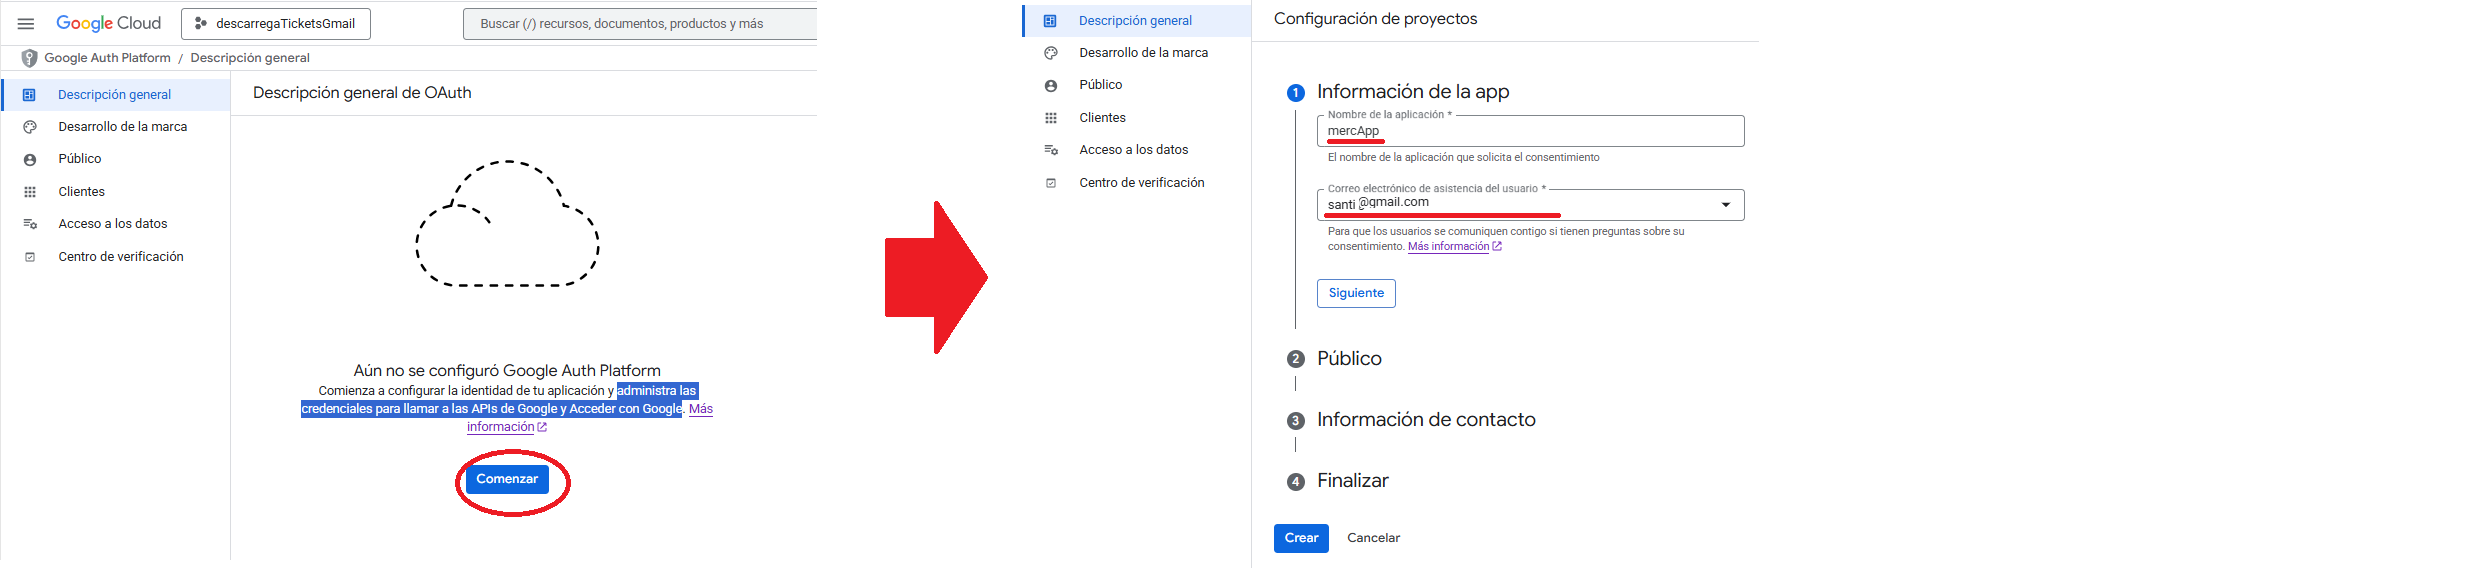
\includegraphics[width=1\linewidth]{img/googleCloudD.png}
		\label{fig:googleCloudD}
	\end{figure}
	\FloatBarrier
	
	\noindent \textbf{PASO 4: Crear credenciales OAuth 2.0 para Web}
	\vspace{.1em}
	\hrule
	\vspace{.5em}
	
	Al pinchar en el círculo verde de la imagen \ref{fig:googleCloudD} obtenemos una ventana de configuración\footnote{Podemos llegar a esa ventana de configuración -es decir al contenido de la figura \ref{fig:googleCloudE}- del mismo modo si optamos por seguir una ruta por menús: \textit{Apis y servicios} (buscador) $\rightarrow$ \textit{credenciales} $\rightarrow$ \textit{+ crear credenciales} $\rightarrow$ \textit{ID de cliente Oauth}.} que nos permite modificar aquello para lo que sirve el \textit{ClientID}\footnote{El clientID identifica la aplicación que corre en el cloud que estamos creando (descarregaTicketsGmail). Sin él un usuario no podría llegar a hacer una llamada autenticándose con su cuenta de google hacia nuestro cloud.} como podemos ver en la imagen \ref{fig:googleCloudE}. A través de esta configuración tenemos que decirle a Google de qué dominios y de qué puertos puede recibir llamadas para autenticarse.
	
	
	\FloatBarrier
	\setlength{\belowcaptionskip}{3pt}
	\begin{figure}[H]
		\centering
		\caption{Configuración de Client ID.  $|$ \textbf{*}: http://localhost:5500 no habrá manera que funcione porque saltará la Content-Security-Policy que impide que hagamos llamadas desde local. Si no hubiera esta CSP, para desarrollo estaría bien, pero en producción habría que tener mucho cuidado, porque si alguien accediese al código con cualquier IP de localhost (cualquier ordenador del mundo) y un vscode con live server, podría hacer llamadas usando el cloud a nuestro nombre  $|$ \textbf{**}: En producción añadiremos otros orígenes que el de localhost: hay que poner aqui la IP fija de nuestro servidor o el dominio (no tenemos uno todavía), siempre habilitando protocolo HTTPS, sino, no funcionará. $|$ \textbf{***}: Para el despliegue en local tendremos que confiar en github pages para hacer la extracción.}
		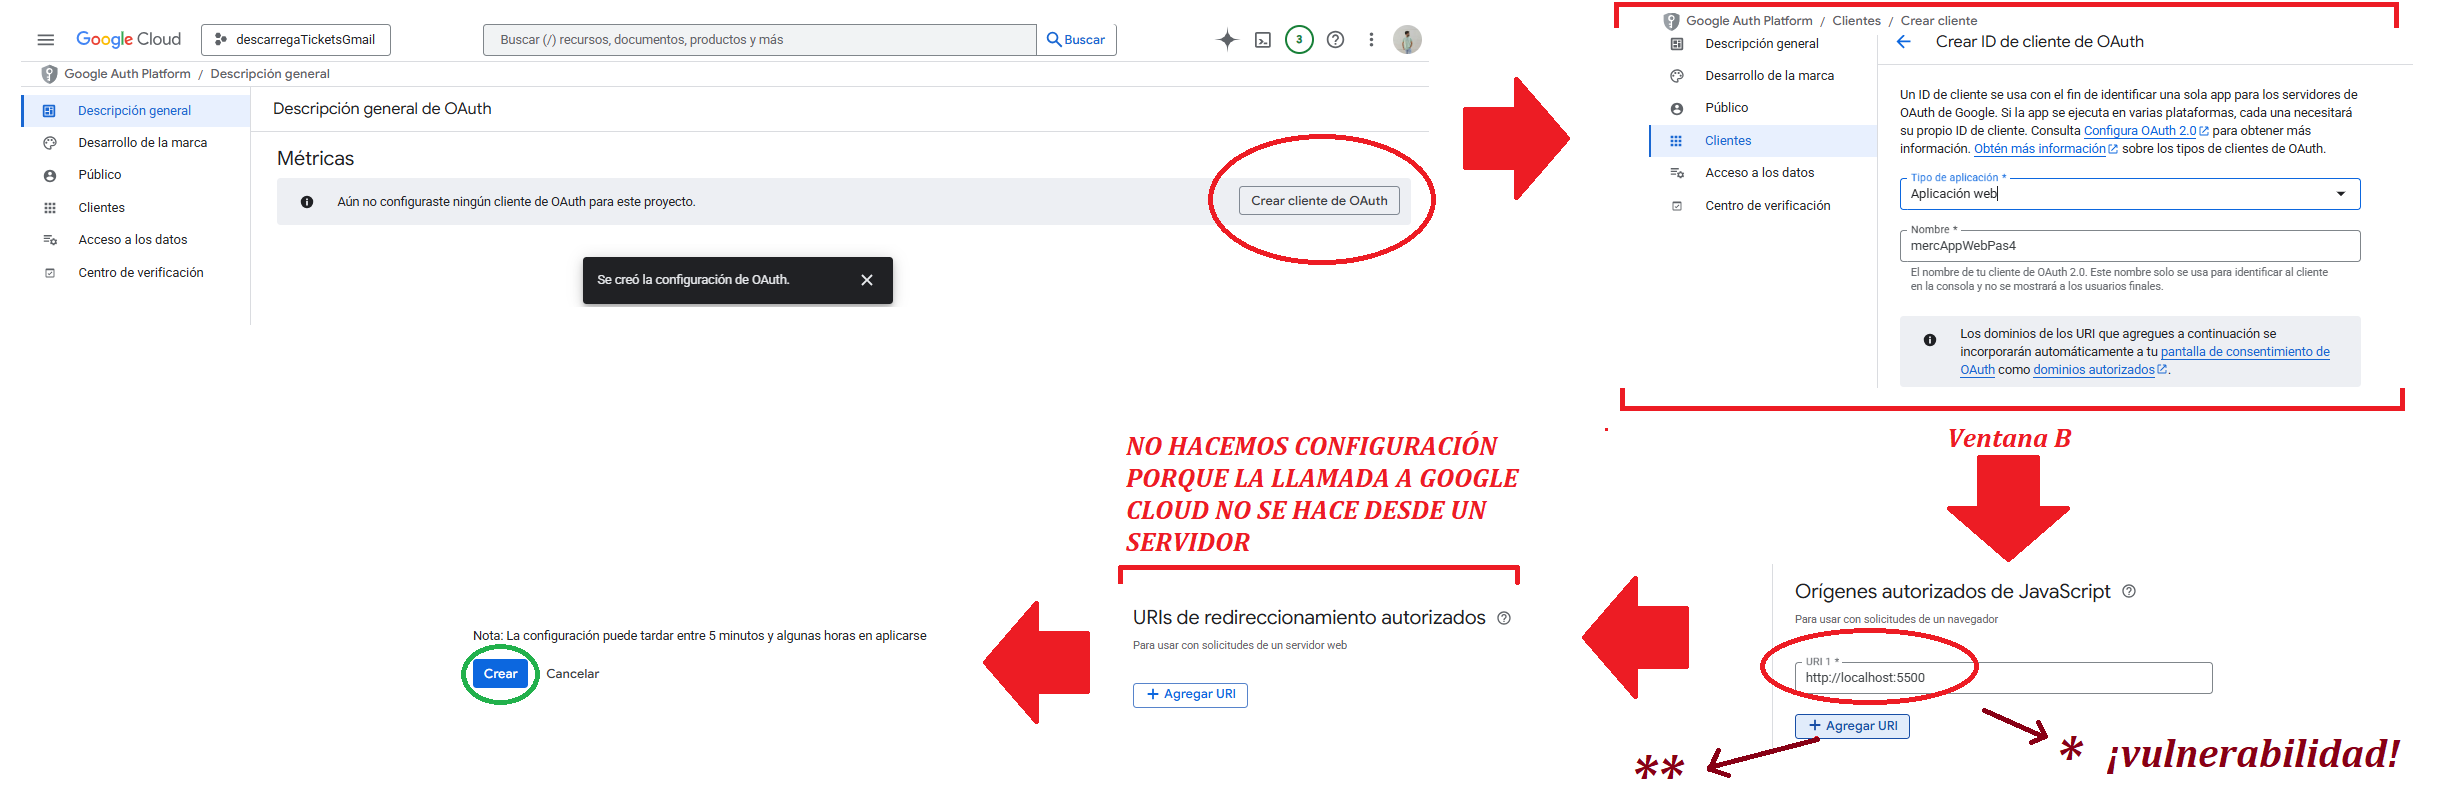
\includegraphics[width=1\linewidth]{img/googleCloudE.png} 
		\label{fig:googleCloudE}
	\end{figure}
	\FloatBarrier
	
	
	
	Después de la configuración hecha en la imagen \ref{fig:googleCloudE} esta será la vista que tendremos si entramos en el buscador, en las \textbf{credenciales} y vemos los ID de clientes OAuth2.0:
	
	\FloatBarrier
	\setlength{\belowcaptionskip}{3pt}
	\begin{figure}[H]
		\centering
		\caption{Vista de la aplicación cloud después de la creación del ClientID}
		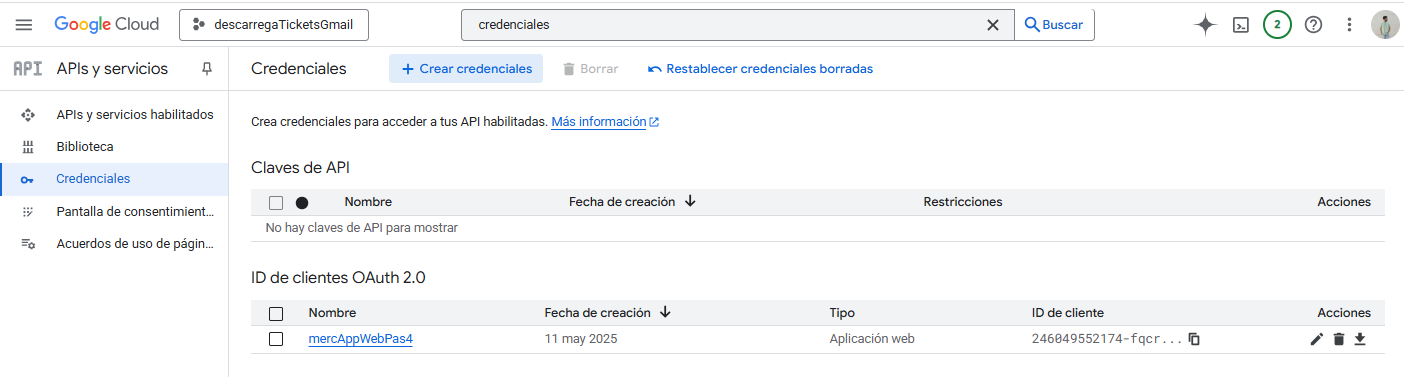
\includegraphics[width=1\linewidth]{img/googleCloudF}
		\label{fig:googleCloudF}
	\end{figure}
	\FloatBarrier
	
	
	
	\noindent \textbf{PASO 5: Añadir usuarios al listado de usuarios permitidos (desarrollo)}
	\vspace{.1em}
	\hrule
	\vspace{.5em}
	
	Google no deja que cualquier usuario pueda autenticarse con el client ID. Para ello o bien hacemos lo del paso 6 (solo para producción, porque requiere una aplicación ya hecha y justificar a google su uso) o bien \textbf{Guardamos una lista de usuarios autorizados a autorizarse} -valga la redundancia- para que así puedan leer su gmail y descargar sus tickets automáticamente. Esto lo haremos así: Yo añadiré el correo electrónico gmail donde Mercadona me manda los tiquets digital (ver figura \ref{fig:googleCloudB}) y con eso la autenticación será posible, por ahora, solo para este correo.
	
	\FloatBarrier
	\setlength{\belowcaptionskip}{3pt}
	\begin{figure}[H]
		\centering
		\caption{Añadir usuario que podrá autenticarse.}
		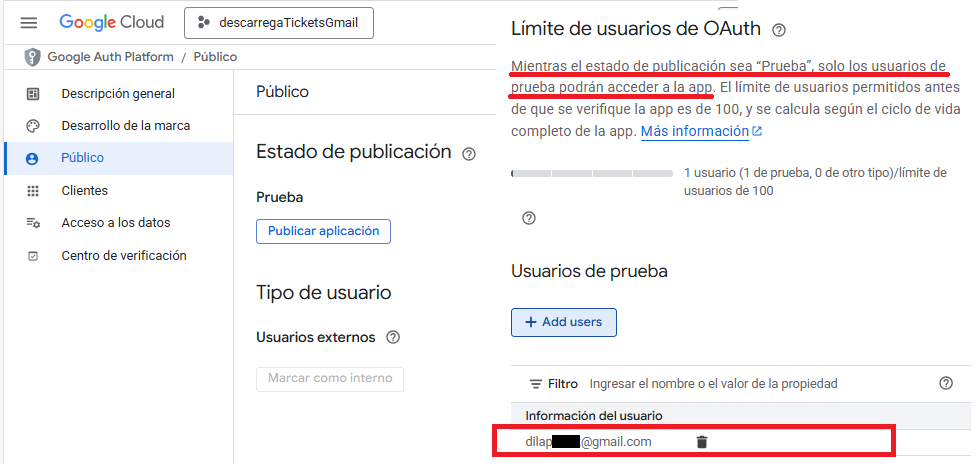
\includegraphics[width=1\linewidth]{img/googleCloudB}
		\label{fig:googleCloudB}
	\end{figure}
	\FloatBarrier
	
	A continuación podemos ver en la figura \ref{fig:googleCloudI} qué pasa cuando tratamos de acceder a autenticarnos en google:
	
	
	
	
	\FloatBarrier
	\setlength{\belowcaptionskip}{3pt}
	\begin{figure}[H]
		\centering
		\caption{\textbf{IZQUIERDA}: tratamos de loguearnos con un usuario que no esta entre los usuarios de prueba. \textbf{DERECHA}: intentamos acceder con el correo que sí está entre los usuarios de prueba y google nos informa que estamos queriendo consultar los mensajes de correo electrónico y su configuración.}
		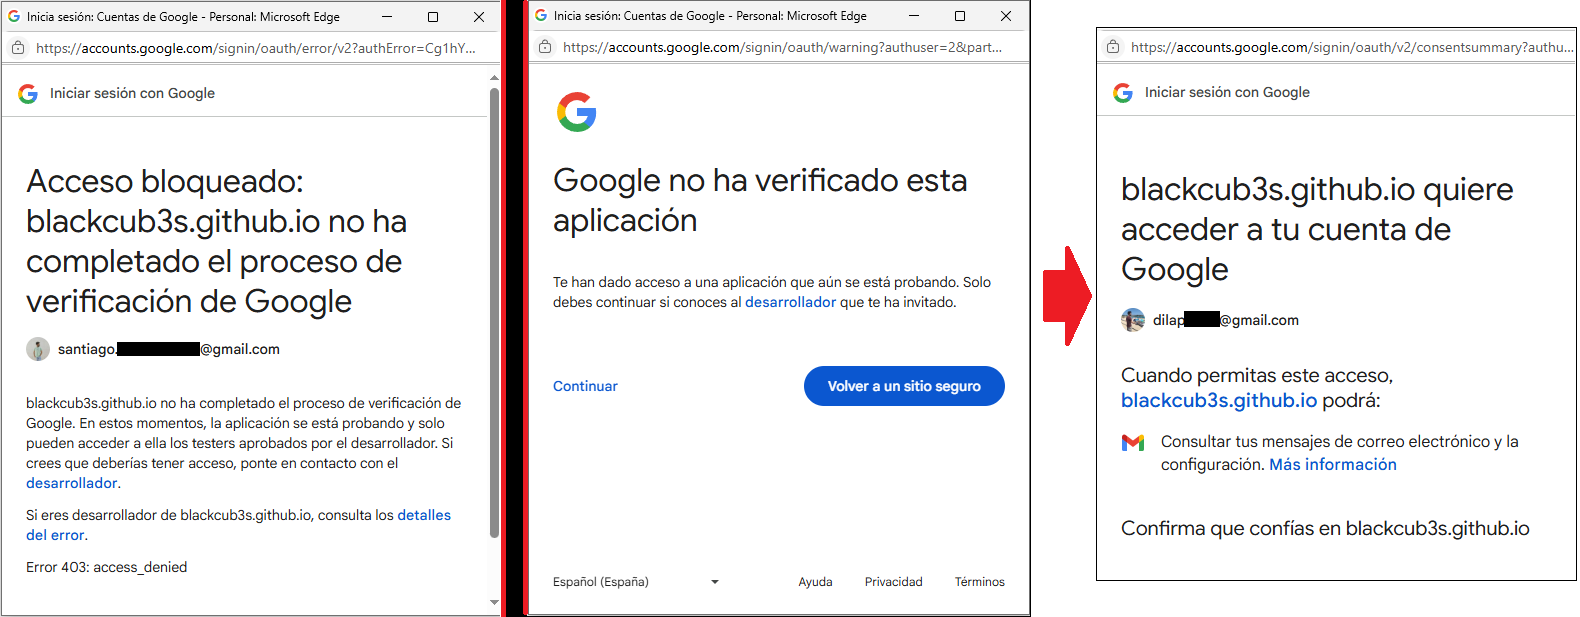
\includegraphics[width=1\linewidth]{img/googleCloudI}
		\label{fig:googleCloudI}
	\end{figure}
	\FloatBarrier
	
	
	
	
	\noindent \textbf{PASO 6: Validar la aplicación descargaTicketsGmail para que cualquier usuario externo pueda usarla (solo en producción y DESPUÉS de autorización expresa de Google).}
	\vspace{.1em}
	\hrule
	\vspace{.5em}
	
	
	Importante mencionar que para que cada usuario pueda acceder a su gmail programáticamente tendremos que habilitar un scope de permisos denominado \textit{gmail.httponly} y verificar la aplicación en el cloud, siguiendo dentro de donde estabamos. Si no lo hiciéramos, tal y como está la configuración de ``usuarios externos'' , por ahora, solo podríamos conseguir que un usuario usase nuestra aplicación cloud de descarga de pdfs del correo mediante el \textbf{Client ID} (que estará en el pas4 del navegador) si también estuviese añadido manualmente a una \textit{lista de verificación} de nuestro cloud.
	
	Esto lo que haría sería que no nos permitiría escalar la aplicación web\footnote{Si os fijáis en la figura \ref{fig:googleCloudD} donde pone Usuarios externos, tenemos una letra pequeña debajo donde se deja claro que por defecto el servicio cloud que acabamos de configurar solo admite usuarios que estén en esa lista.}. Para solucionarlo tenemos que añadir el scope necesario como vemos en la figura \ref{fig:googleCloudG}:
	
	\FloatBarrier
	\setlength{\belowcaptionskip}{3pt}
	\begin{figure}[H]
		\centering
		\caption{Ahora vamos a \textit{``Apis y servicios''} $\rightarrow$ \textit{``Credenciales''} clicamos en la credencial oauth2 creada ``mercAppWebPas'' y en acceso a los datos clicamos en agregar permisos. Añadimos el permiso pertinente que encontramos mediante la adición de un ``scope''- Para ver los scopes podemos acceder al link ``más información'', que nos lleva a \href{https://developers.google.com/identity/protocols/oauth2/scopes?hl=es_419}{ésta página}, y de ahí copiar el scope necesario (usamos \textbf{gmail.readonly}) y lo actualizamos con el boton azul marcado en el círculo verde de la imagen.}
		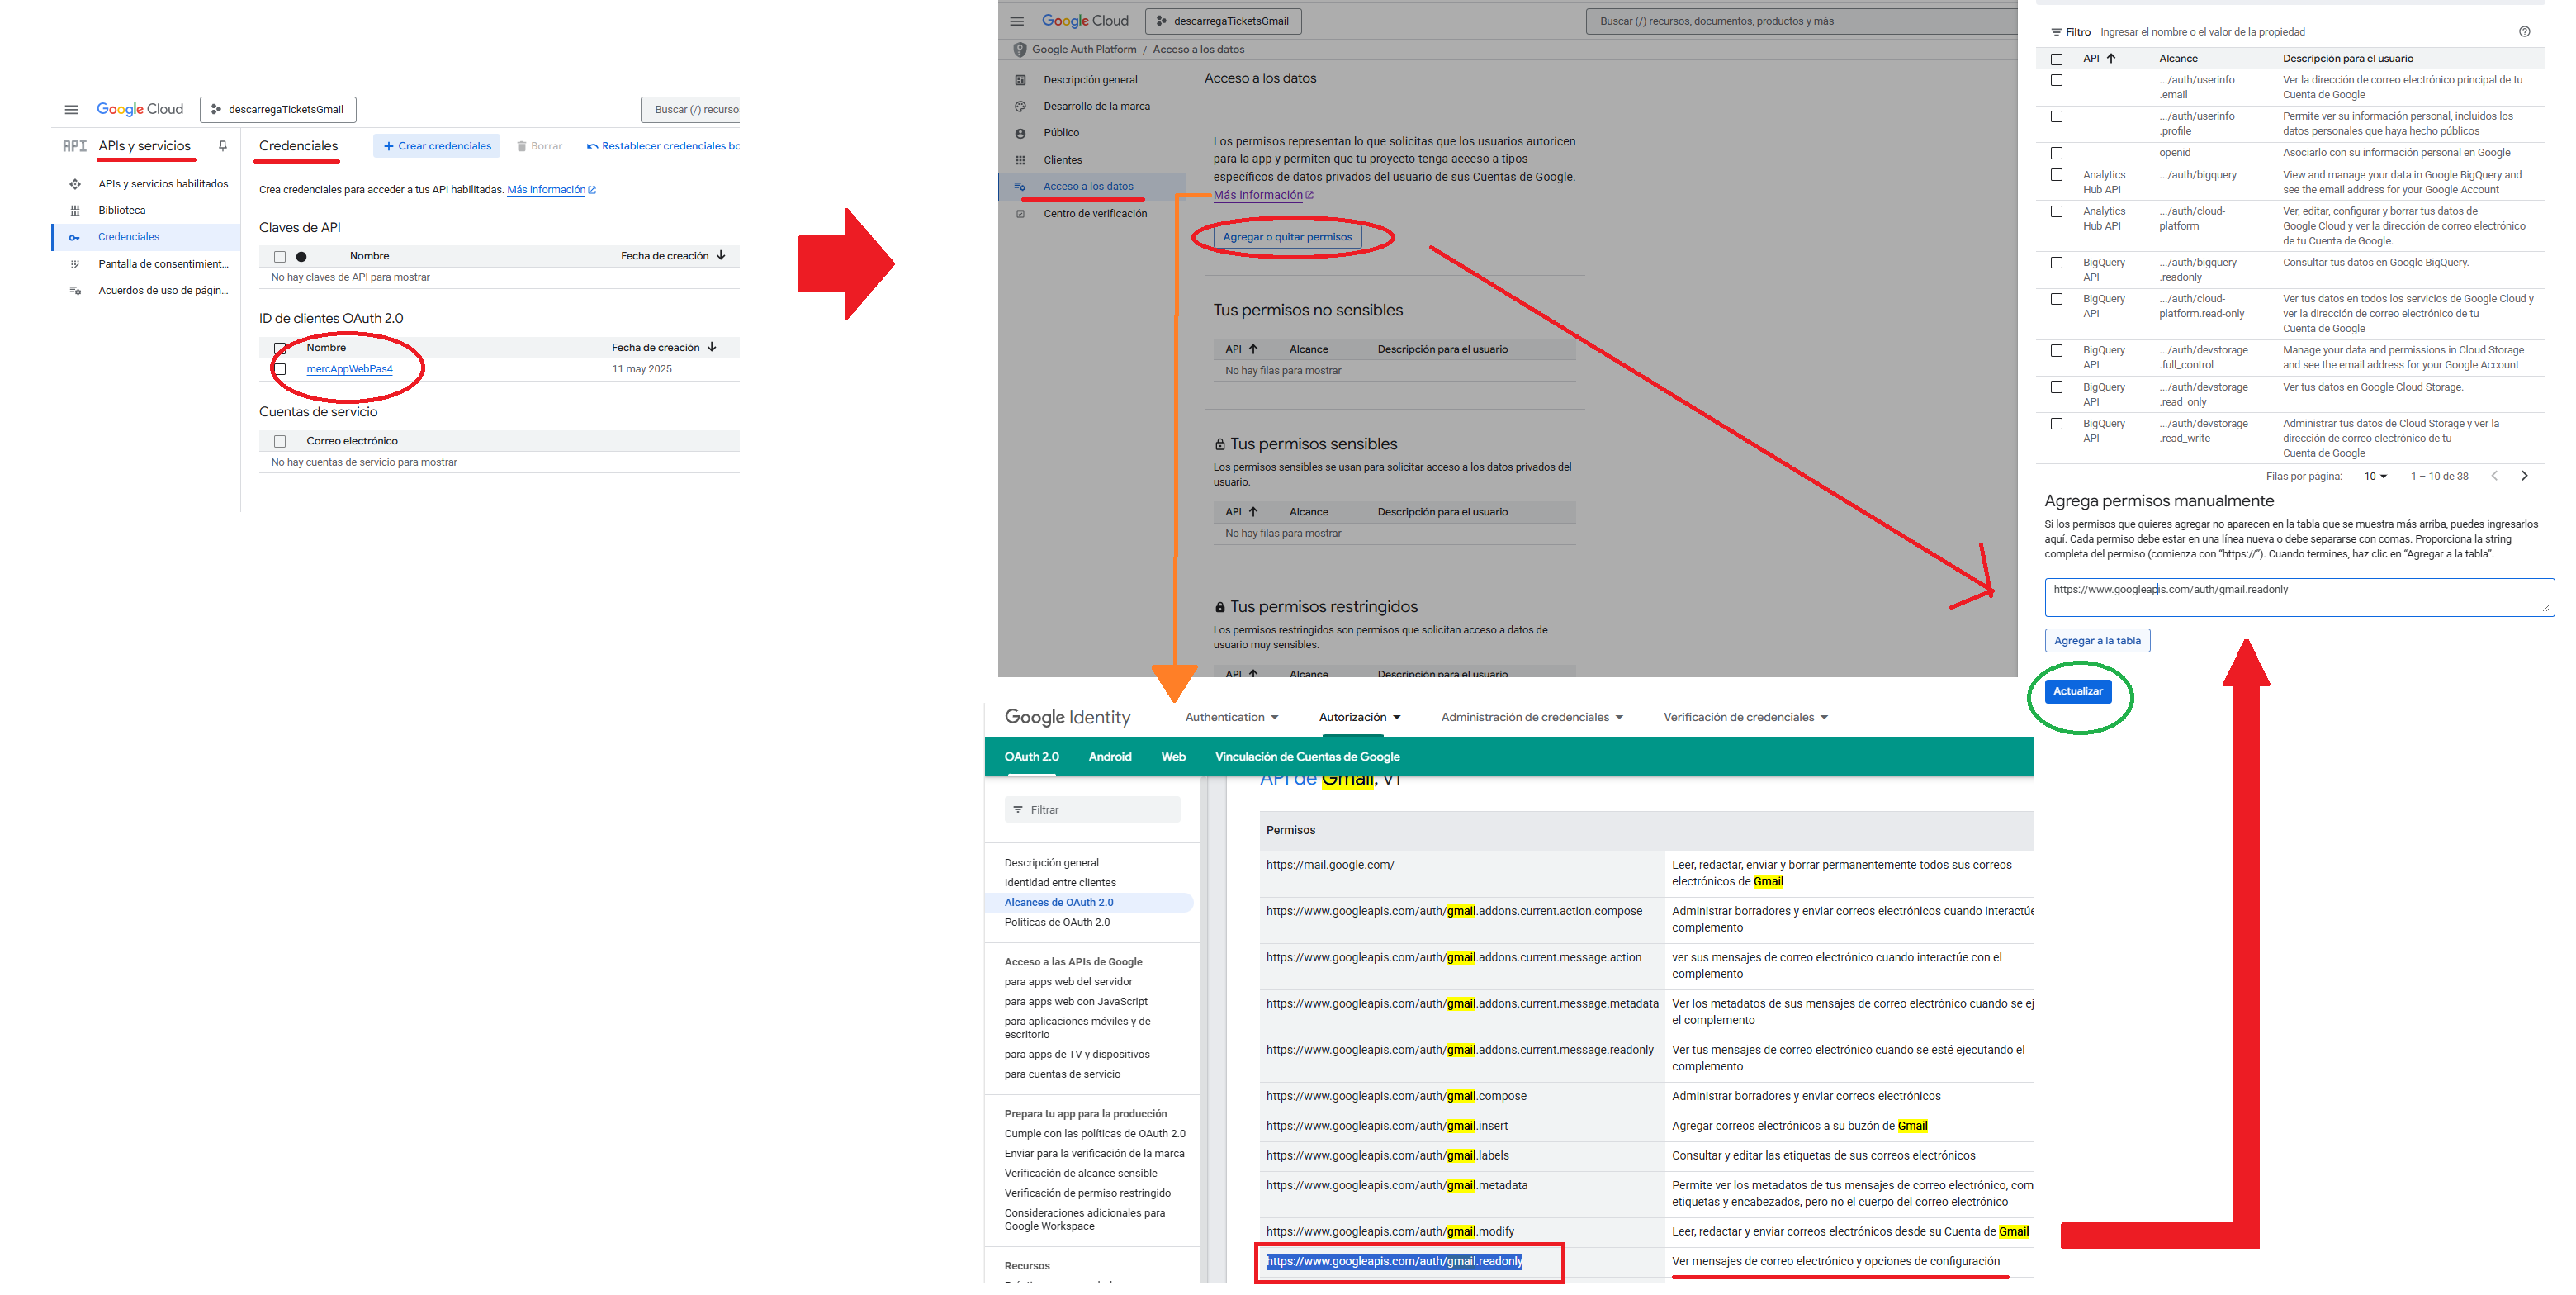
\includegraphics[width=1\linewidth]{img/googleCloudG}
		\label{fig:googleCloudG}
	\end{figure}
	\FloatBarrier
	
	Después de darle a actualizar en la imagen \ref{fig:googleCloudG} tenemos que guardar esta configuración. Para ello seguimos los pasos de la imagen \ref{fig:googleCloudH}:
	
	
	\FloatBarrier
	\setlength{\belowcaptionskip}{3pt}
	\begin{figure}[H]
		\centering
		\caption{Último paso para poder permitir que los usuarios de nuestra aplicación puedan acceder a leer SUS correos electrónicos una vez autenticados, con oauth2. Esta vez vamos a \textit{``Apis y servicios''} $\rightarrow$ \textit{``Credenciales''} $\rightarrow$ \textit{``MercAppWebPas4''} $\rightarrow$ \textbf{\textit{``Acceso a los datos''}} y le damos al \textbf{botón guardar}. }
		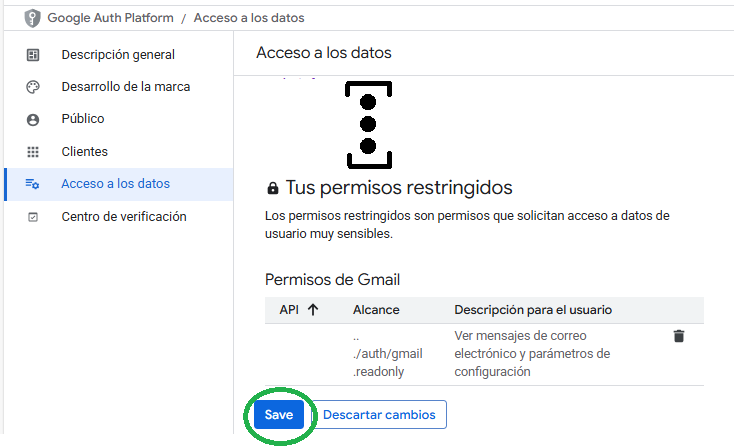
\includegraphics[width=1\linewidth]{img/googleCloudH}
		\label{fig:googleCloudH}
	\end{figure}
	\FloatBarrier
	
	Y el último caso es validar. Que google tiene que dar el vistobueno. Sin embargo asumo que esto no va a pasar, al menos no en plazo, con lo cual, directamente solo podremos usar los correos (por ahora solo uno) en el listado de usuarios permitidos mostrado en el PASO 5, para descargar los tickets digitales.
	
	
	\chapter{Evaluación y Conclusiones Finales} %OBLIGAT
	

	
	
	
	

	
	
	
	
	
	
	
	
	
	
	
	
	
	
	
	
	
	
	
	
	
	
	
	
	
	
	
	
	
	
	
	
	
	
	
	
	
	
	
	
	\chapter{ANEXO}
	\label{chap:anexo} % Esta es la etiqueta de referencia
		
			
		\section{Flujo de trabajo habitual en git}
		\label{sec:anexoFlujoGit}
		
\begin{lstlisting}[language=bash, basicstyle=\ttfamily\small]
	


# trabajamos con el proyecto y se introduce
# en el staging area
git add -A 

# creamos rama para aglutinar los cambios
git branch backEnd

# cambiamos a la rama que acabamos de crear
git checkout backEnd

# guardamos los cambios como nodos dentro de
# la rama con la que desarrollamos.	
git commit -m "commit 1"  	
git commit -m "commit 2"
# [...]
git commit -m "commit n"

#cambiamos a rama main local y luego integramos cambios
git checkout main
git merge backEnd

#Subimos los cambios al repo remoto
git push origin main 

	
\end{lstlisting}
		
	
\pagebreak

		
		
		\section{Diferencias de seguridad: JWT vs SESSID en cookies seguras}
		\label{sec:anexo_JWTvsSESSIONS}
						
			\FloatBarrier
			\begin{table}[h]
				\centering
				\begin{tabular}{|p{4cm}|p{5cm}|p{5cm}|}
					\hline
					\textbf{Característica} & \textbf{JWT en cookies seguras} & \textbf{Session ID en cookies seguras} \\
					\hline
					\textbf{Seguridad contra XSS} & Más seguro si la cookie tiene \texttt{HttpOnly} y \texttt{Secure}, ya que no es accesible desde JavaScript. & Más seguro si la cookie tiene \texttt{HttpOnly} y \texttt{Secure}, ya que no es accesible desde JavaScript. \\
					\hline
					\textbf{Seguridad contra CSRF} & Puede ser vulnerable si la cookie no tiene \texttt{SameSite=Strict}. & Menos vulnerable si la cookie tiene \texttt{SameSite=Strict}. \\
					\hline
					\textbf{Estado en el servidor} & Stateless (no hay estado en el servidor, el JWT contiene toda la información). & Stateful (el servidor mantiene una sesión activa asociada con el Session ID). \\
					\hline
					\textbf{Escalabilidad} & Mejor escalabilidad porque no requiere almacenamiento de sesiones en el servidor. & Menos escalable, ya que el servidor debe manejar las sesiones activas. \\
					\hline
					\textbf{Expiración y revocación} & Difícil de revocar antes de que expire, a menos que se implemente una lista negra en el servidor. & Fácil de invalidar eliminando la sesión en el servidor. \\
					\hline
					\textbf{Uso con JavaScript} & No accesible desde JavaScript si la cookie tiene \texttt{HttpOnly}. & No accesible desde JavaScript si la cookie tiene \texttt{HttpOnly}. \\
					\hline
				\end{tabular}
				\caption{Comparación de seguridad entre JWT y Session ID almacenados en cookies seguras con HttpOnly=True.}
				\label{tab:jwt_vs_session}
			\end{table}
			\FloatBarrier
	
		\pagebreak
		
		
		\section{Clases para crear y verificar JWTs}
		\label{sec:anexoCreacionYverificacionJWT}
	
	
\subsection{Clase JWT}


\begin{lstlisting}[language=Java, basicstyle=\ttfamily\tiny, keywordstyle=\color{magenta}]
	
//NO INSTANCIEM AQUESTA CLASSE MAI. LA FEM ABSTRACTA
@Component
public abstract class JwtUtil {
	
	//es la clau privada de 256 bits com a minim per encriptar el token (tant el d'acces com el de refresh)
	//veure debat http://bit.ly/3RmBGIK
	protected static String clauSecreta;
	
	public JwtUtil() {
		this.clauSecreta = "a8f7d9g0b6c3e5h2i4j7k1l0m9n8p6q3r5s2t1u4v0w9x8y7z";
	}
	
	//METODE QUE PARSEJA EL TOKEN JWT COMPLET. VERIFICA LA FIRMA I EXTRAU LES CLAIMS (parells clau valor en el payload).
	protected Claims getClaims(String token) {
		return Jwts.parser()
		.setSigningKey(clauSecreta.getBytes())
		.build()
		.parseClaimsJws(token)
		.getBody();
	}
	
}






\end{lstlisting}


				

\subsection{Clase Refresh Token}

\begin{lstlisting}[language=Java, basicstyle=\ttfamily\tiny, keywordstyle=\color{magenta}]

@Component
public class RefreshToken extends JwtUtil {
	
	private static int tExpDies;
	
	public RefreshToken() {this.tExpDies = 7;}
	
	// FINALITAT DEL METODE: Refrescar el token d'acces que genera generaAccesToken().
	public String generaRefreshToken(String correu, int idUsuari) {
		Map<String, Object> dadesExtraApayload = new HashMap<>();
		dadesExtraApayload.put("idUsuari", idUsuari);
		//posar mes dades al payload si es necessari
		
		return Jwts.builder()
		.setClaims(dadesExtraApayload) //dades customitzades
		.setId(String.valueOf(UUID.randomUUID().toString())) //id unic per a token. Per traSSSabilitat
		.setSubject(correu)           //guardo nom subjecte (dins "sub")
		.setIssuedAt(new Date())      //data creacio
		.setExpiration(new Date(System.currentTimeMillis() + tExpDies*86400*1000))  //expiracio
		.signWith(SignatureAlgorithm.HS256, clauSecreta.getBytes())
		.compact();
	}
}

\end{lstlisting}


\subsection{Clase Access Token}
\begin{lstlisting}[language=Java, basicstyle=\ttfamily\tiny, keywordstyle=\color{magenta}]

@Component
public class AccessToken extends JwtUtil {
	
	private static int tExpM; //minuts per a exprirar el token
	
	public AccessToken() {this.tExpM = 10;}
	
	//FINALITAT: Generar un JWT d'acces.
	public String genera(String correu, int idUsuari, byte permisos) {
		Map<String, Object> dadesExtraApayload = new HashMap<>();
		dadesExtraApayload.put("permisos", permisos);
		dadesExtraApayload.put("idUsuari", idUsuari);
		
		return Jwts.builder()
		.setClaims(dadesExtraApayload) //dades customitzades
		.setSubject(correu)            //guardo nom subjecte (clau "sub")
		.setIssuedAt(new Date())       //data creacio (clau "iat" payload)
		.setExpiration(new Date((System.currentTimeMillis() / 1000 + (tExpM * 60)) * 1000))
		.signWith(SignatureAlgorithm.HS256, clauSecreta.getBytes())
		.compact();
	}
}
	
				
\end{lstlisting}
	
		\section{Clases de seguridad}
		
		\subsection{Clase ConfiguracioSeguretat.java}
		\label{sec:anexoConfiguracioSeguretat}
		
				
		\begin{lstlisting}[language=java, basicstyle=\ttfamily\footnotesize, keywordstyle=\color{magenta}]
package miApp.app.seguretat;


@Configuration
@EnableMethodSecurity 
@PreAuthorise
public class ConfiguracioSeguretat {
	
  private final FiltreAutenticacioJwt jwtAuthenticationFilter;

  public ConfiguracioSeguretat(FiltreAutenticacioJwt jwtAuthenticationFilter) {
    this.jwtAuthenticationFilter = jwtAuthenticationFilter;
  }

  @Bean
  public SecurityFilterChain securityFilterChain(HttpSecurity http) 
      throws Exception {
	http
	.csrf(csrf -> csrf.disable())
	.authorizeHttpRequests(auth -> auth
	.requestMatchers("/api/correusUsuaris").hasRole("ADMIN")
	.requestMatchers("/api/usuaris/*").hasAnyRole("USER", "ADMIN")
	.requestMatchers("/api/usuaris").hasRole("ADMIN")                       
	.requestMatchers("/api/nreUsuaris").hasAnyRole("USER", "ADMIN")        
	.requestMatchers("/api/*/contrasenya").hasAnyRole("USER", "ADMIN")
	.requestMatchers("/api/**").permitAll()
	)
	.addFilterBefore(jwtAuthenticationFilter,
	 UsernamePasswordAuthenticationFilter.class);
	
	return http.build();
    }
	
	
  }
		\end{lstlisting}
	
	
	
		\subsection{Controlador con restricciones aplicadas}
		\label{sec:detallSeguretatControlador}
		
		La restricción aplicada es @PreAuthorize. Solamente usuarios que tengan rol administardor o bien usuarios que contengan el id == principal (el propio id del usuario autenticado) podrán cambiar la contraseña:
		
\begin{lstlisting}[language=java,  basicstyle=\ttfamily\footnotesize, keywordstyle=\color{magenta}]


@PatchMapping("usuaris/{id}/contrasenya")
@PreAuthorize("hasRole('ADMIN') or #id == principal") 
public ResponseEntity<HashMap<String, String>> actualitzaContrasenya(
	@PathVariable("id") int id, @Valid 
	@RequestBody ActualitzaContrasenyaDTO dto) {
	Optional<Usuari> usuariActualitzatOPTIONAL =
	 serveiUPP.actualitzaContrasenya(dto, id);
	HashMap<String, String> resposta = new HashMap<>(); 
	if (usuariActualitzatOPTIONAL.isPresent()) {
		resposta.put("mensaje", "Contrasena actualizada correctamente.");
		return new ResponseEntity<>(resposta, HttpStatus.OK); //200 OK
	} else {
		resposta.put("mensaje", "Usuario no encontrado.");
		return new ResponseEntity<>(resposta, HttpStatus.NOT_FOUND);  //404 NOT FOUND
	}
}

\end{lstlisting}
			
			
		
		
		\section{Diagrama réplica netflix}
		\label{sec:anexo_diagramaNetflix}
		
		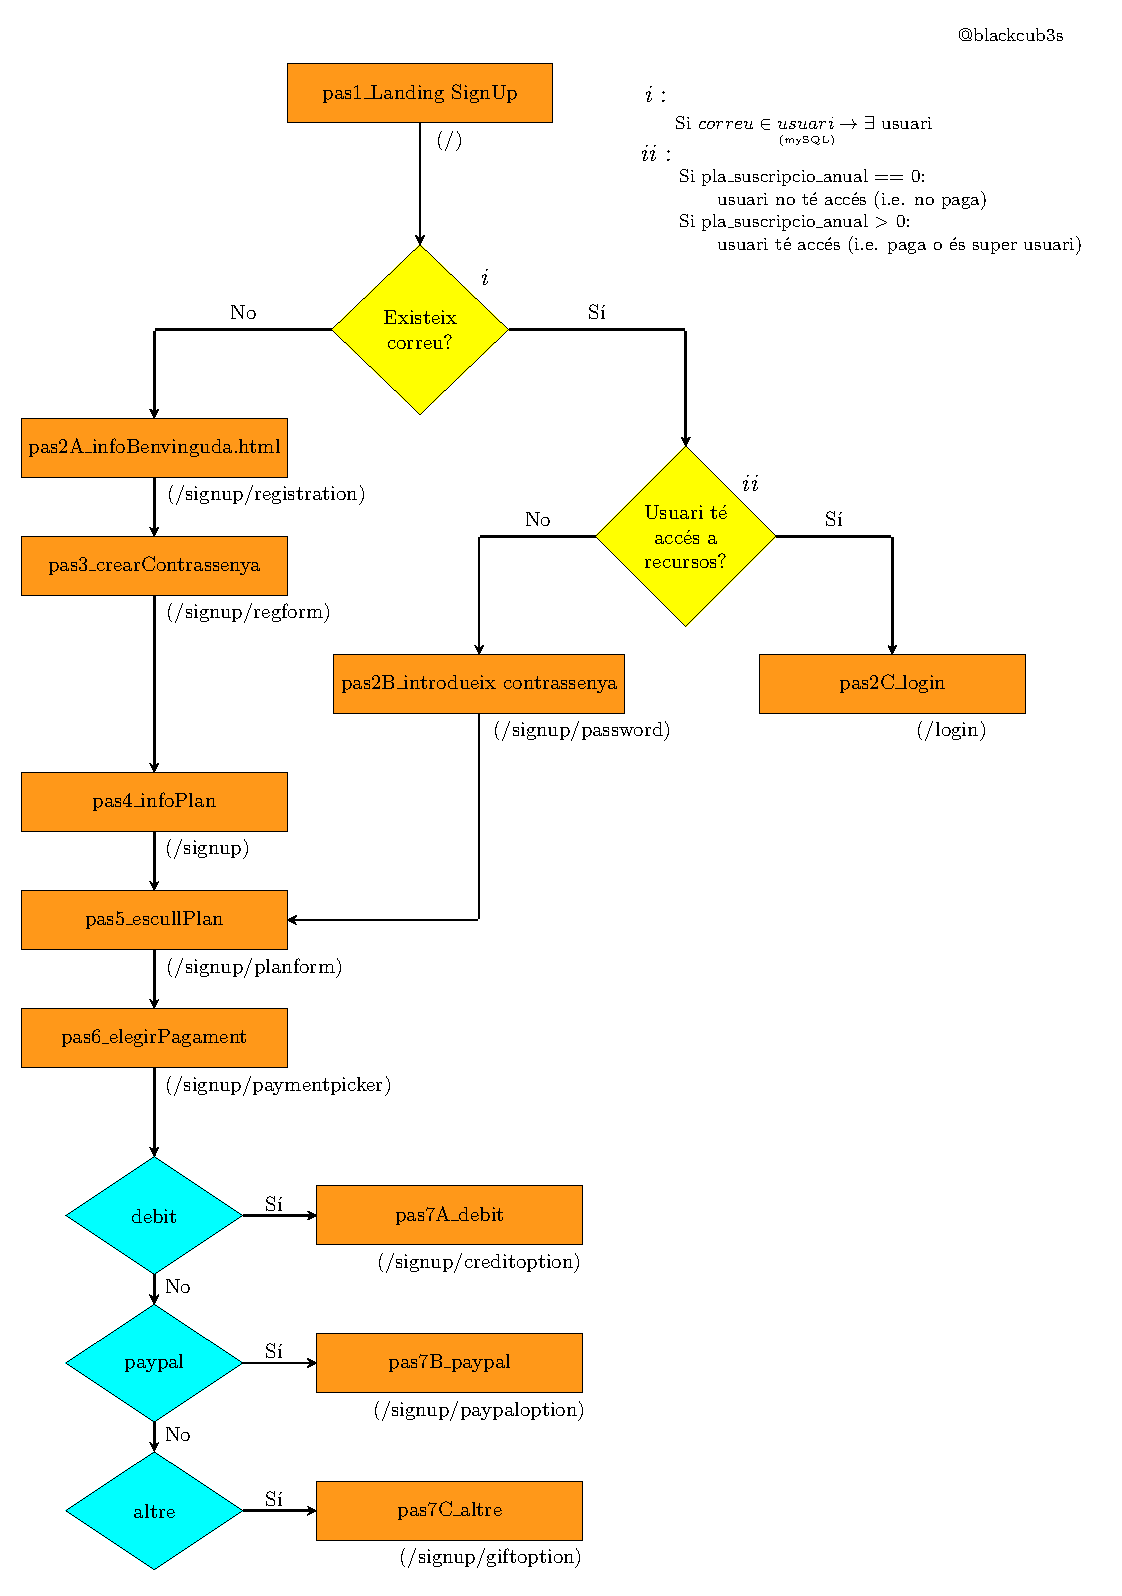
\includegraphics[width=1\textwidth]{img/diagramaTikzDefinitiuV2.pdf}

		NOTA: El lector puede ver el proceso de creación de este diagrama en el repositorio \href{https://github.com/blackcub3s/diagramaTikz}{diagramaTikz}. También puede ver una explicación del diagrama a continuación:
		
		Este diagrama se puede entender del siguiente modo:
		
		\begin{enumerate}
			\item Cada rectángulo de color naranja es una página estática \texttt{.html} de lo que sería una réplica de la página de registro de netflix.
			\item Cada rombo de fondo amarillo es una decisión que se hará dentro del back-end de Spring Boot, dado que requiere hacer consultas a la BBDD y contiene datos sensibles.
			\item Los rombos de fondo azul se decidirán en el front-end en tanto que sus decisiones no requieren consultar información personal en la base de datos y no precisan, por lo tanto, del uso del back-end (y, además, no se explicarán en este \textit{readme}).
			\item El paréntesis que incluye la extensión de una URL debajo de cada rectángulo naranja es cada página de Netflix cuyo comportamiento y, en menor medida, aspecto, se ha intentado replicar en el archivo \texttt{.html} del rectángulo naranja que le es contiguo. Por ejemplo, el archivo \texttt{pas2A\_infoBenvinguda.html} de este proyecto es una réplica de la página especificada en el paréntesis \texttt{netflix.com/signup/registration} y el usuario llegará a ella a través del proceso de registro gracias a la aplicación de una lógica de back-end similar a la que usa Netflix.
		\end{enumerate}

		
	

		\section{Diagrama enrutamiento mercApp}
		\label{sec:anexo_diagramaEnrutamietnoMercApp}

		\section{Aspectos ventajosos de separar front-end y back-end (SoC)}
		\label{sec:SoCVENTATJES}
			\begin{itemize}
			\setlength{\itemsep}{.0em}
			\item \textbf{Responsabilidad única (SRP)}: Cada módulo debería hacer una sola cosa ($\{$Frontend $\rightarrow$ interfaz$\}$, $\{$Backend $\rightarrow$ procesamiento$\}$). 
			\item \textbf{mantenibilidad}: Al usar una arquitectura modular cada parte puede evolucionar por separado. Podemos desplegar solo el front o el back. En el futuro podremos cambiar el front-end de archivos estáticos por un front-end con Angular, por ejemplo.
			\item \textbf{Escalabilidad}: Según la carga podemos escalar independientemente ambas partes del proyecto. Por ejemplo, poner los archivos estáticos (html, css y js del front-end) en un servidor para servirlos rápidamente como nGinx \cite{nginx} (supuestamente más rápido que Apache). Dejar en el tomcat embedido de springboot el procesamiento del back-end y si hay problemas de escalabilidad escalar este independientemente en AWS, AZURE, o en un servidor propio según sea más conveniente.
			\item \textbf{Reutilización}: Un backend puede servir varios front-ends (no solo web, sino móvil también). El mismo front-end podemos reutilizarlo luego para otra aplicación con un back-end en otro lenguaje por ejemplo.
		\end{itemize}
		
	\section{Captura proyecto desarrollo interfaces}
	
	\FloatBarrier
	\begin{figure}[H]
		\centering
		\caption{Detalle del paginador de swiper del proyecto de desarrollo de interfaces.}
		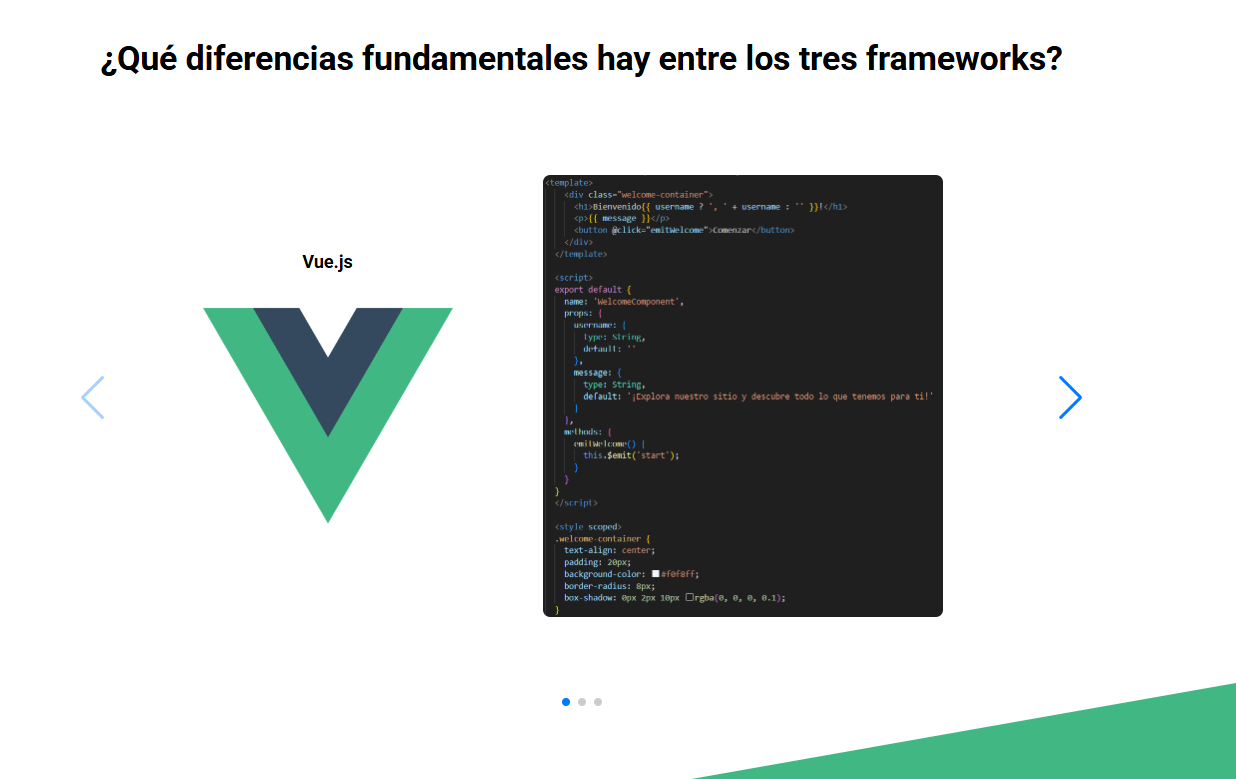
\includegraphics[width=1\linewidth]{img/swiperFront.png}

		\label{fig:swiperFront}
	\end{figure}
	\FloatBarrier
	
	\pagebreak
	\section{Creación del icono mercapp pequeño: IA con Gimp}
	\label{sec:edicionMercAppIconoPequenyo}
	
	\noindent \textbf{NOTA:} \textit{Podéis regresar al punto de la memoria del que os hemos redirigido clicando en el link de secció siguiente:} \ref{sec:iconoMercappPetitMEMORIAPPAL}
	
	\FloatBarrier
	\setlength{\belowcaptionskip}{3pt}
	\begin{figure}[H]
		\centering
		\caption{Proceso completo de creación del icono pequeño de mercApp. El proceso involucra IA generativa y pequeñas ediciones en gimp para retirar canal alpha, pintar el fondo de la delta y añadir una parte redonda con fondo blanco para que se vea en la barra de navegación negra. Existe un icono con la delta blanca para barra de navegación negra que aquí no mostramos.}
		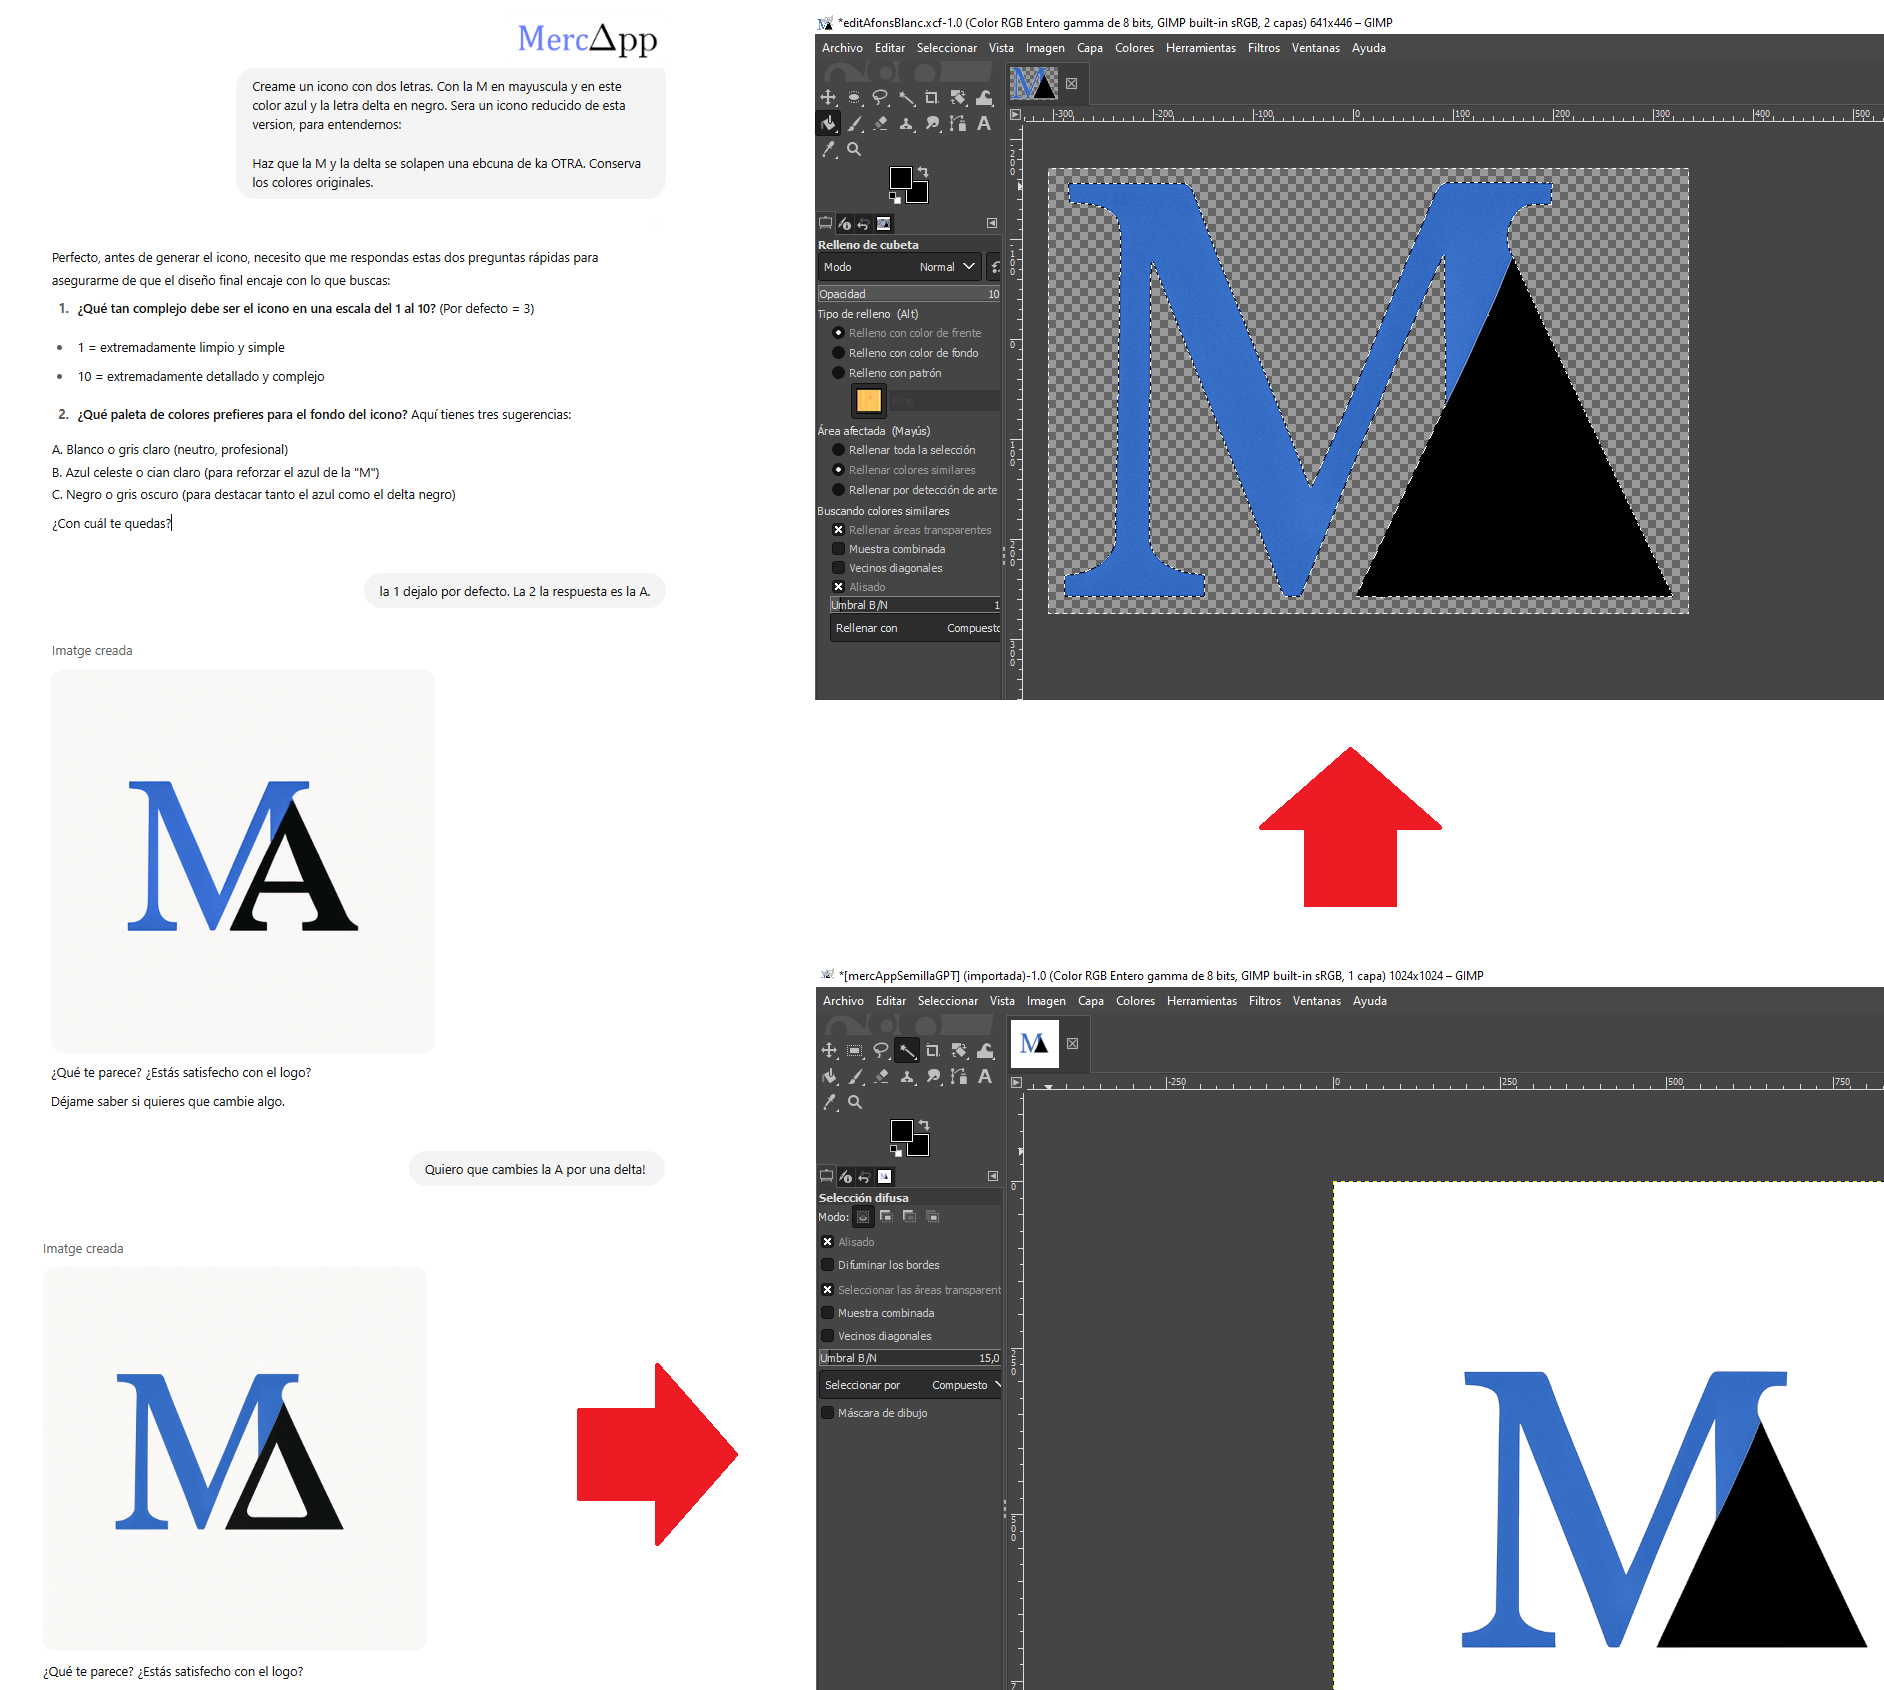
\includegraphics[width=1\linewidth]{img/edicionMercAppIconoPequenyo.png}
		\label{fig:edicionMercAppIconoPequenyo}
	\end{figure}
	\FloatBarrier
		
	% Bibliografía (\chapter(6. Bibliograifa) como implicito)
	\addcontentsline{toc}{chapter}{7. Bibliografía} 
	\bibliographystyle{unsrt}  % Estilo de bibliografía no ordenats (Segons ordre aparicio en text)
	\bibliography{referencias} % Nombre del archivo .bib  extensión
	
	
	

	\endgroup
	
	
	\section{Google Cloud: descargar tickets digitales mediante cloud}
	\label{sec:googleCloud}
	
		NOTA: clica aquí \ref{sec:pas4googleAPIclient} para regresar al texto que referenció este anexo.\\
		
	
		Los pasos a seguir para obtener el ClientID necesario para habilitar usuarios a la descarga de tickets digitales es acceder a \href{https://cloud.google.com}{https://cloud.google.com/} e introducir la información de pago (si ya tenemos pagos periódicos a Google por, por ejemplo, compra de almacenamiento a google drive no habrá que añadirlos). Fijémonos en lo que está disponible: 300 dólares de créditos gratuito durante tres meses. Como vemos en la figura \ref{fig:googlecloud1}.
		
		\FloatBarrier
		\begin{figure}[H]
			\centering
			\caption{Crear cuenta gratuita de google cloud}
			\label{fig:googlecloud1}
			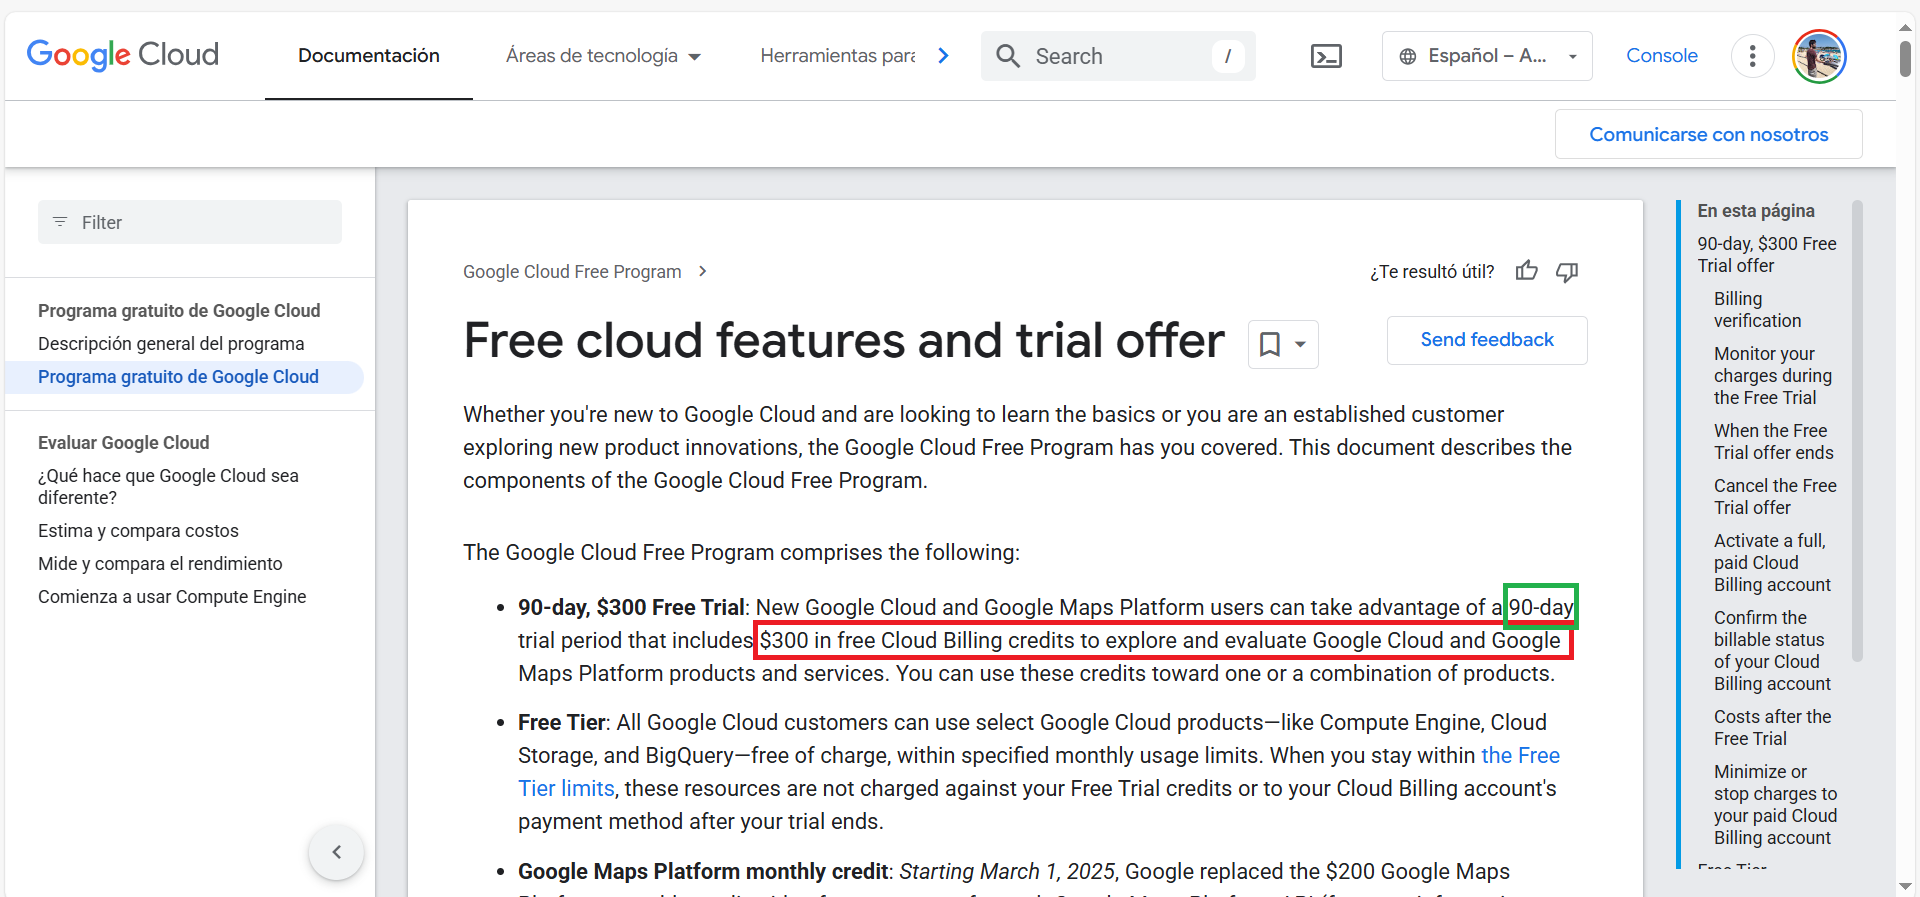
\includegraphics[width=1\linewidth]{img/googleCloud1.png}
		\end{figure}
		\FloatBarrier
		
		
		Si consultamos los servicios gratuitos en \href{https://cloud.google.com/free/docs/free-cloud-features?authuser=2#free-tier-usage-limits}{esta página} tenemos muchos. De ellos los que pueden servirnos para nuestro caso particular podrían ser \textbf{App Engine} y \textbf{Cloud run}. Ambos tienen un free tier distinto. Después de extraer la información detallada de \href{https://cloud.google.com/run/docs/overview/what-is-cloud-run?authuser=2&hl=es-419}{Cloud run} y de \href{https://cloud.google.com/appengine/docs/an-overview-of-app-engine?authuser=2&hl=es-419}{app engine} hay un claro ganador en cuanto a costes para nuestro caso de uso: el primero (ver figura \ref{fig:googleCloud2}).
		
		\FloatBarrier
		\begin{figure}[H]
			\centering
			\caption{Dos servicios con free tier que nos pueden ser de utilidad para nuestra aplicación. El que a priori sería más económico sería \textit{cloud run} porque asegura que el proceso escalará a cero cuando no esté en uso, y nos permite activarlo solamente con un evento web (cuando el usuario se acabe de registrar y pida acceso a los tickets)}
			\label{fig:googleCloud2}
			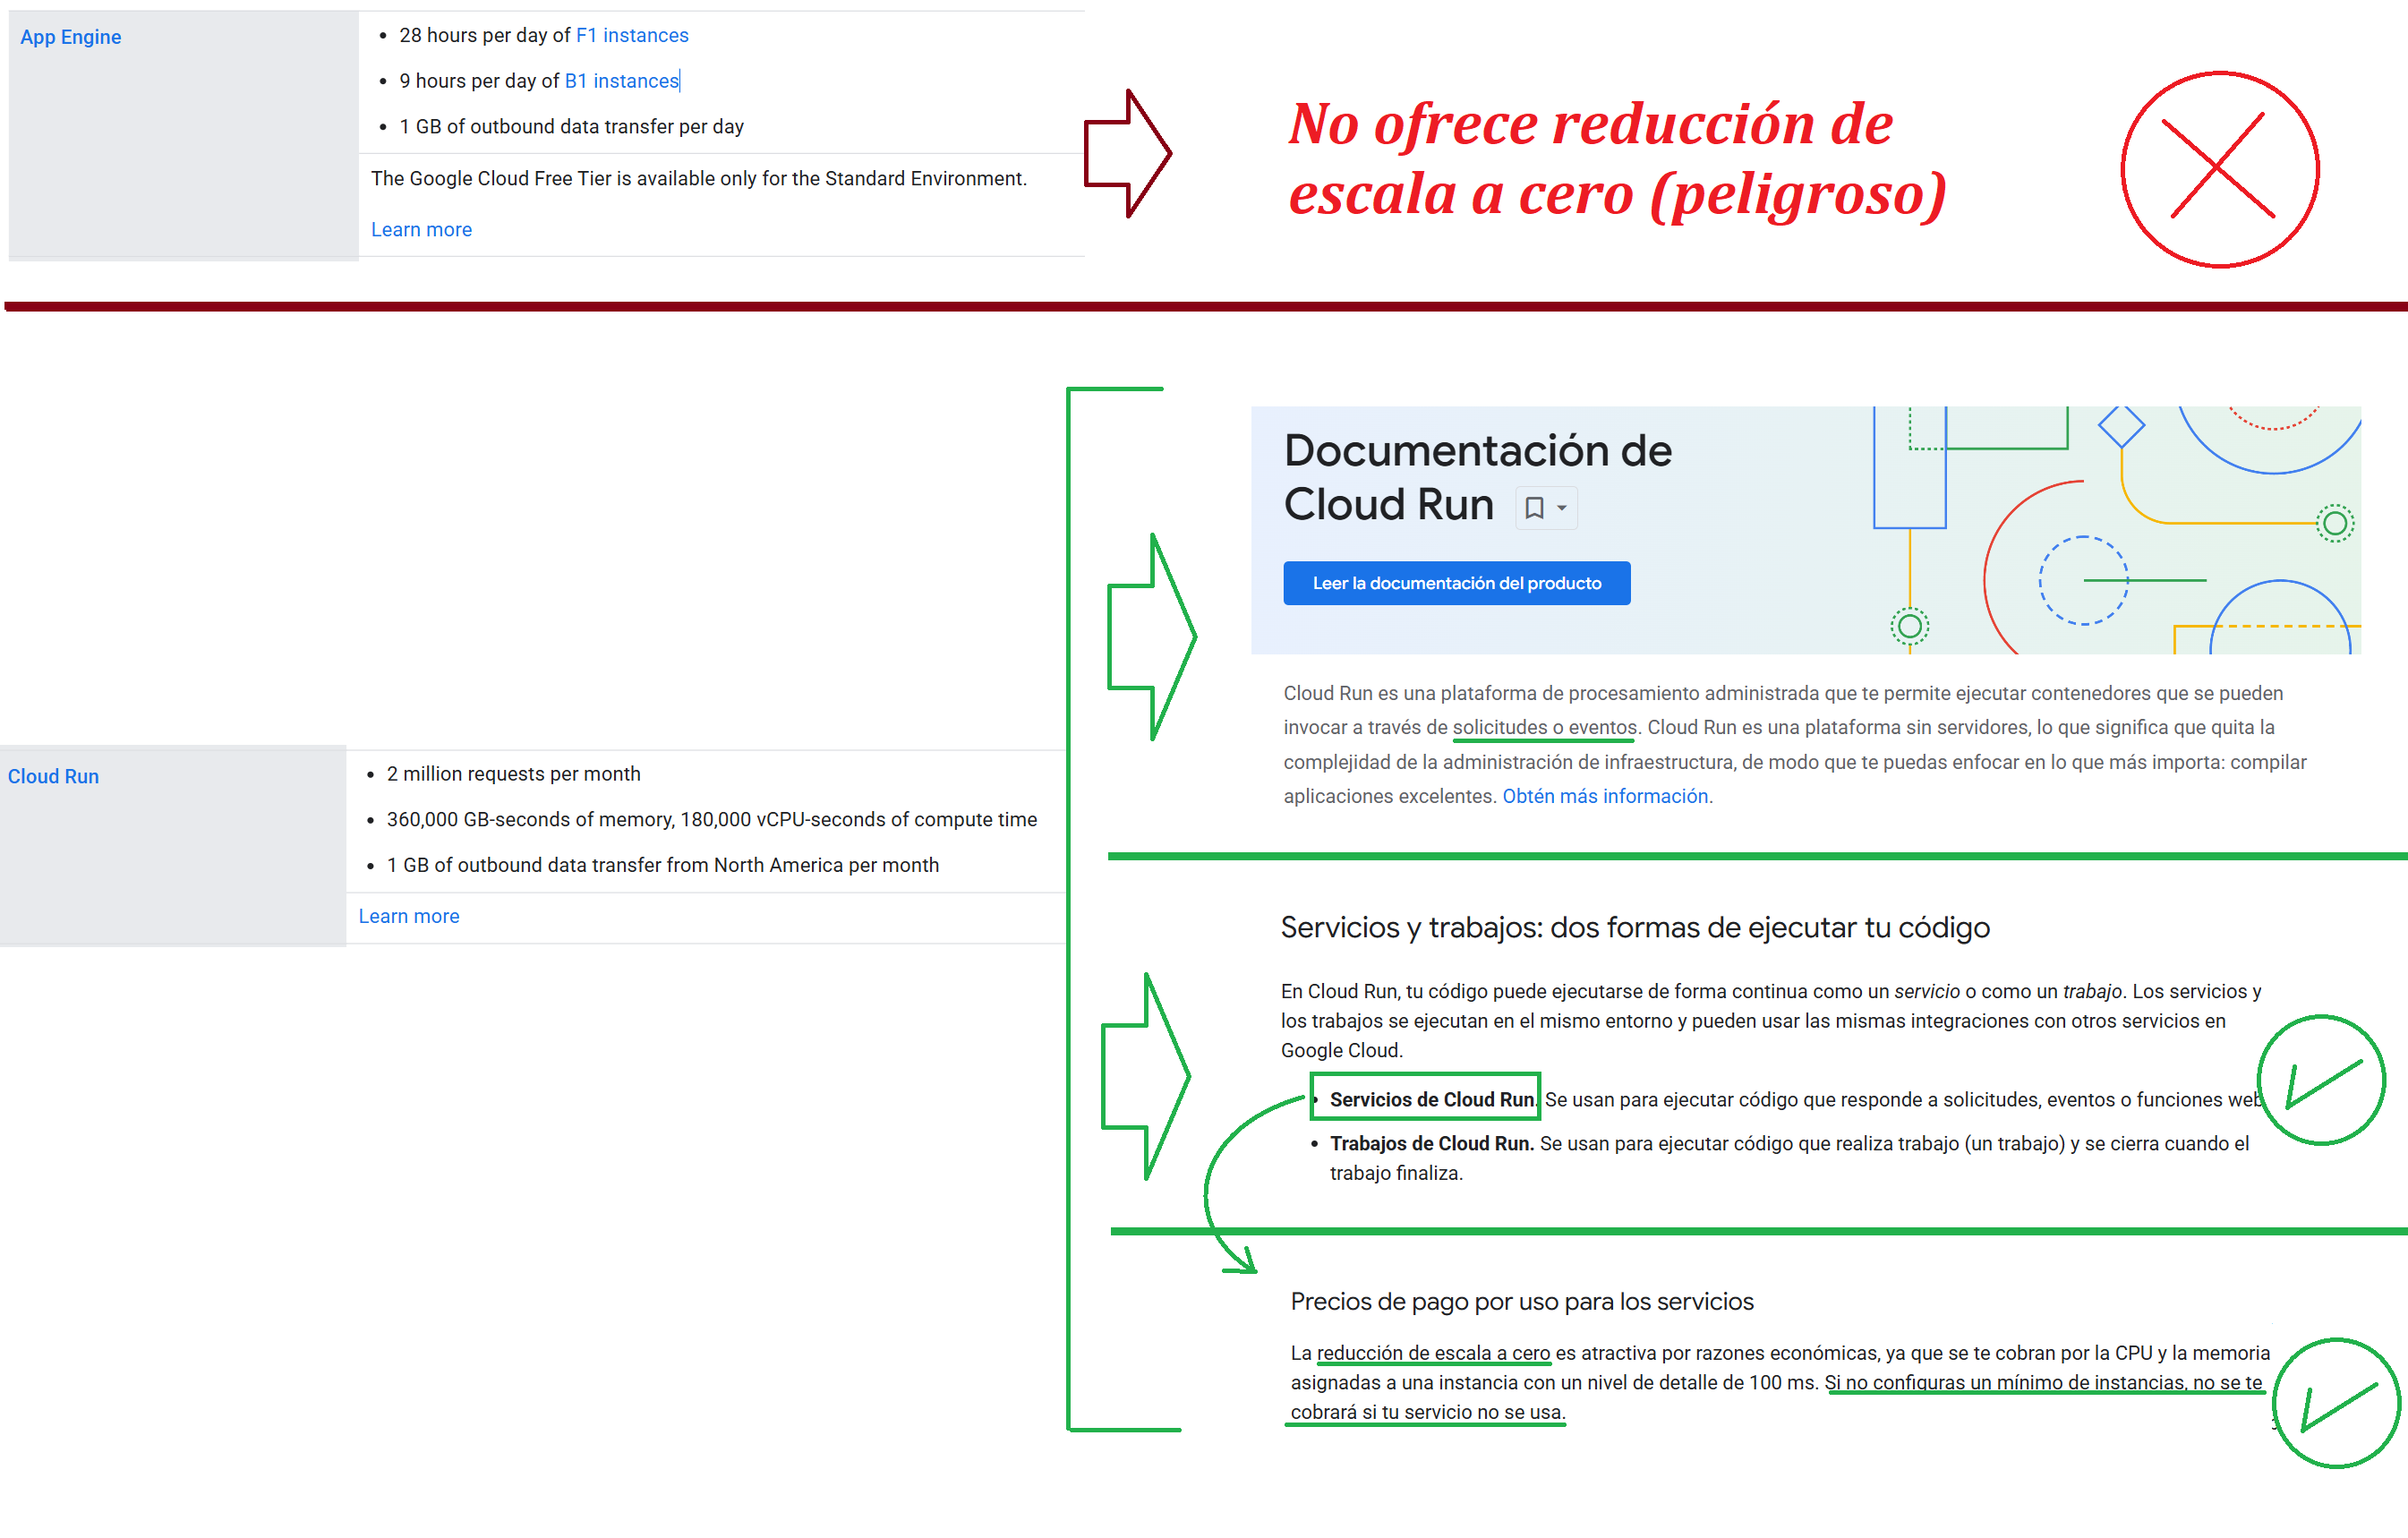
\includegraphics[width=1\linewidth]{img/googleCloud2.png}
		\end{figure}
		\FloatBarrier
		
	\textbf{Cloud run requiere contenerizar una aplicación y subirla al cloud. Sin embargo, aunque podría funcionar para nuestro caso particular, nada gana el hacerlo desde el front end como finalmente se ha hecho.}
		
		
	
	

	
	
\end{document}
